\documentclass[12pt,a4paper]{article}

% ─── Packages ───────────────────────────────────────────────────────────────
\usepackage[a4paper, margin=1in]{geometry}
\usepackage{graphicx}
\usepackage{booktabs}
\usepackage{array}
\usepackage{longtable}
\usepackage{hyperref}
\usepackage{listings}
\usepackage{titlesec}
\usepackage{fancyhdr}
\usepackage{float}
\usepackage{enumitem}
\usepackage{parskip}

% ─── Page Style ─────────────────────────────────────────────────────────────
\pagestyle{fancy}
\fancyhf{}
\rhead{Carefree- Aiding Caretakers}
\lhead{SCD-CEA}
\rfoot{Page \thepage}
\renewcommand{\headrulewidth}{0.4pt}

% ─── Section Formatting ─────────────────────────────────────────────────────
\titleformat{\section}{\large\bfseries}{}{0em}{}[\titlerule]
%\titleformat{\subsection}{\normalsize\bfseries}{}{0em}{}

% ─── Code Listing Style ─────────────────────────────────────────────────────
\lstset{
    basicstyle=\ttfamily\small,
    breaklines=true,
    frame=single,
    numbers=left,
    numberstyle=\tiny,
    showstringspaces=false
}

% ────────────────────────────────────────────────────────────────────────────

\begin{document}

% ─── Title Page ─────────────────────────────────────────────────────────────
\begin{titlepage}
    \centering
    \vspace*{1cm}

    {\Large \textbf{NED University of Engineering \& Technology}}\\[0.3cm]
    {\large Department of Software Engineering}\\[1.5cm]

    \rule{\linewidth}{0.5mm}\\[0.4cm]
    {\LARGE \textbf{Lab Session 13}}\\[0.2cm]
    {\Large Complex Engineering Activity (CEA)}\\[0.2cm]
    {\large PLO5 -- Modern Tool Usage}\\[0.2cm]
    \rule{\linewidth}{0.5mm}\\[1.5cm]

    {\large \textbf{System:} Carefree-Aiding Caretakers}\\[0.7cm]

    \begin{tabular}{ll}
        \textbf{Sunbmitted by:}    & Sarah Raza Rahman(SE-24011)\\
        & Adeena Falah (SE-24014)\\
        & Hafsa Rahman (SE-24021)\\
        & Aiza Samad Khan (SE-24031)\\[0.3cm]
        \textbf{Course Code:}     & SE-312        \\[0.3cm]
        \textbf{Submitted to:}      & Ms. Rafia Shakeel    \\[0.3cm]
        \textbf{Submission Date:} &  \today            \\
    \end{tabular}

    \vfill
\end{titlepage}

\tableofcontents
\newpage

\section{Task 1 -- System Documentation}

\subsection{System Overview}

\subsubsection{Introduction}
CareFree – Aiding Caretakers is a lightweight patient management web application that helps caretakers manage daily 
tasks such as appointment scheduling, task organization, and expense tracking. The system aims to reduce errors, 
improve efficiency, and provide clear visibility into patient care routines. By ensuring transparency in caregiving 
activities, CareFree supports better accountability and trust between caretakers and guardians.

\subsection{System Users}

\begin{itemize}
    \item \textbf{Caretaker:} 
    Caretakers can be certified nursing assistants, unlicensed caregivers with hands-on
experience or just individuals with a background in healthcare or social work.
They look after patients and their daily needs. They might have more than one patient
and need efficient tools to handle.
    \item \textbf{Guardian:} 
    Guardians are family members or legal representatives who oversee patient care.
They do not provide direct care but monitor patient health and are able to
communicate with the caretakers through the app.
\end{itemize}

\subsection{Key Features}

\begin{itemize}
    \item Login and Sign up
    \item Patient Information Management
    \item Appointment Tracking
    \item Caretaker Task Management
    \item Expense Tracker
    \item Notifications
    \item ML Cost Predictor
    \item ML Stress Classifier
    \item Vitals and Symptoms Tracker
\end{itemize}


\subsection{Functional Requirements}

\subsubsection{Sign up}
\begin{itemize}
    \item FR1.4.1.1. The system should allow users to create an account by providing their username, email address, password and role.
    \item FR1.4.1.2. The system should ensure that each email address is unique.
    \item FR1.4.1.3. The system shall confirm account creation to inform users.
\end{itemize}
\subsubsection{Login}
\begin{itemize}
    \item FR1.4.2.1. The system shall match the username and password pairs before authorizing user access.
    \item FR1.4.2.2. The system should redirect users to their respective dashboards i.e. Caretaker and Guardian respectively.
    \item FR1.4.2.3. The system should display an error message incase of incorrect credentials being entered.
\end{itemize}
\subsubsection{Patient Information Management}
\begin{itemize}
    \item FR1.4.3.1. Caretakers can create new patient records by filling out the following fields: Full name, Age, Gender, Height, Weight, Diagnosis, Current medications, Assigned Caretaker ,Guardian contact details, and any special notes. 
\\The system checks if all data types are valid, for example, no letters in the age field, no 
numbers in the name or gender fields, and only supported values for each section. 
    \item FR1.4.3.2. After adding a patient the system will output guardian credentials to the caretaker. 
    \item FR1.4.3.3. Caretakers can update existing patient records, including the patient’s personal 
details entered at the time of creating a new patient record as mentioned in FR1.4.3.1.
    \item FR1.4.3.4. Caretakers can delete patient records, with two options. If a record is permanently 
deleted, it’ll never be accessible again but if a record is archived, it remains accessible 
for future reference but cannot be modified. Archived records will be stored in a 
separate, read-only database accessible only to caretakers. 
    \item FR1.4.3.5. The system allows caretakers to search for patient records, filters by: Name, patient ID, Age, Gender, Assigned caretaker, or any special notes. 
    \item FR1.4.3.6. The system must allow caretakers and guardians to assign or reassign a caretaker, 
validate the change, offer temporary access if needed and save the updates. 
    \item FR1.4.3.7. The system will allow caretakers to upload and securely store prescriptions and lab 
reports within a patient’s record. These documents will be linked to the patient’s 
profile and can be modified only by caretakers. Guardians will be able to view (but not 
download, upload, modify, or delete) these documents. 
    \item FR1.4.3.8. The system will provide reminders when: A patient record is missing important details, a patient’s medical history requires an update 
    \\These reminders will appear on the dashboard. 
    \item FR1.4.3.9. After each patient visit, the caretaker logs details such as the date, time, reason for the 
visit, observations, and any prescribed treatments. The system securely stores this 
information in the patient's record, ensuring a complete history of care. 
    \end{itemize}
    
\subsubsection{Appointment Tracking}
\begin{itemize}
    \item FR1.4.4.1. Caretakers should be allowed to create and schedule Patient Schedules, which will be 
stored in a Patient Appointment table in the database, by entering the following 
information: Patient ID (out of the ones stored in the Caretaker Information table), Nature of the appointment (doctor’s, physical therapy, social appointments, etc.), Appointment date, Time of the appointment, Specification notes 
    \item FR1.4.4.2. Caretakers can mark the appointment as one of the following options on the day of the 
appointment: Completed, Postponed, To be decided, Canceled. 
    \item FR1.4.4.3. If the caretaker chooses to postpone, the system will automatically give the user two 
options The caretaker will be asked to add a new day, complying with which they will 
specify a date that will be stored in the database OR Mark the appointment as to be 
decided.
    \item FR1.4.4.4. Ensure that any appointments added are for the future by using the system’s clock. 
Both the time and date should refer to the future. Appointments should be at least 10 
minutes in the future. 
    \item FR1.4.4.5. Display a confirmation message on the screen signaling the following\\ 
1. Addition: “New Entry added” \\
2. Deletion: “Confirm Deletion of Entry” \\
3. Edition: “Confirm Action” while also displaying the changes made. 
    \item FR1.4.4.6. Both caretakers and guardians will be able to view the information regarding the 
medications and appointments for the patient. Guardians will have permission to 
view only. 
    \item FR1.4.4.7. The system should automatically schedule and store appointments, and reminder 
notifications should be available to the user as recommendations in the Notifications Feature. 
\end{itemize}

\subsubsection{Caretaker Task Management}
\begin{itemize}
    \item FR1.4.5.1. Allow caretakers to view, create, delete, and update tasks. This information will be 
available to the caretaker to view under the task name.\\ 
1. They will also be able to view the description. \\
2.  And the most recent time of the upcoming task. \\
3. Guardians will be able to view the Tasks related to their patient.
    \item FR1.4.5.2. While creating and scheduling a task, caretakers shall enter the following information, 
which will be saved in the “Tasks” table: Name of the task, Patient ID, Date, Time, Priority, Progress, Description, Frequency out of the following options: Daily, 2 times a week, on alternate days, once weekly, once monthly.  
    \item FR1.4.5.3. No more than 1 urgent task can be kept at a single time. In an attempt to add a second 
urgent task, the user will be asked to choose one of the three options: \\
1. The system asks to either downgrade the other task to moderate, \\
2. Replace the previous task with the new one, OR \\
3. Cancel the new request. 
    \item FR1.4.5.4. The system will not allow tasks with the same name; in case of this, it will ask the 
caretaker to: \\
1. Either change the frequency of the already available task OR \\
2. Replace the task with a new one in its name. 
    \item FR1.4.5.5. To track the progress of these tasks, there will be a dialog box at the time of the task: 
mark them as completed or incomplete. \\
1. If the task is incomplete, the caretaker will be asked to either reschedule or delete 
the task. \\ 
2. For tasks with multiple occurrences, 15 minutes before every occurrence, the 
progress will automatically be marked as incomplete. 
\end{itemize}

\subsubsection{Expense Tracker}
\begin{itemize}
    \item FR1.4.6.1. Caretakers can log expenses in categories (for example related to medical care, food).
    \item FR1.4.6.2. The system shall allow caretakers to edit an existing expense entry by selecting it 
from the list and modifying its details (e.g., amount, category, payment method). 
    \item FR1.4.6.3. Caretakers should be able to delete an expense entry.
\end{itemize}

\subsubsection{Notification}
\begin{itemize}
    \item FR1.4.7.1.  Caretakers can set multiple types of notifications (e.g. Task Alerts and Appointment Alert). 
    \item FR1.4.7.2. Notifications for tasks are configured to appear at the time of tasks.
    \item FR1.4.7.3. Notifications for appointments appear 2 hours before the appointment time. 
    \item FR1.4.7.4. Caretakers can view, edit, or delete existing notifications from a dedicated screen. 
    \item FR1.4.7.5. Notifications appear only when the caretaker is signed in to the application.
    \item FR1.4.7.6. Caretakers can acknowledge, dismiss, and mark alerts as "Resolved"or "Unresolved" 
for tracking. 
\end{itemize}

\subsubsection{ML Medical Cost Predictor}
\begin{itemize}
    \item FR1.4.8.1. The ML cost predictor shall use a supervised learning algorithm (gradient boosting) to 
ensure that predictions are accurate. 
    \item FR1.4.8.2. The ML model shall take as input the patient’s age, gender, the region they live in, their 
smoking habits, and the diseases they have from the Patient Information database.  
    \item FR1.4.8.3. The model shall output a floating number equating to the expected yearly medical 
cost of each Patient.  
    \item FR1.4.8.4. The calculated cost shall be stored in the database with the respective patient IDs.   
    \item FR1.4.8.5. If the data in the database is incomplete, the system shall prompt the caretaker to 
complete patient information before making a prediction.  
    \item FR1.4.8.6. Only the caretaker can prompt the system to make a prediction, while the guardian 
can view it once the prediction has been made.
    \item FR1.4.8.7.  The model shall be trained again every six months on newly collected data to ensure 
model accuracy.  
    \item FR1.4.8.8. The data shall always be anonymised before using it to train the model, ensuring 
privacy and security of data. 
\end{itemize}

\subsubsection{ML Stress Classifier}
\begin{itemize}
    \item FR1.4.9.1. The ML stress classifier shall use a supervised learning algorithm (decision tree) to 
ensure that predictions are accurate. 
    \item FR1.4.9.2. The ML model shall take as input the patient’s hours of sleep, their sleep quality, systloc and diastolic blood pressure, physical activity, daly steps, heart rate and BMI category as entered by the caretaker.  
    \item FR1.4.9.3. The model shall output one of three categories: Low, Moderate and High. 
    \item FR1.4.9.4. Only the caretaker can prompt the system to make a prediction based on the data entered.   
    \item FR1.4.9.5.  The model shall be trained again every six months on newly collected data to ensure 
model accuracy.  
    \item FR1.4.9.6. The data shall always be anonymised before using it to train the model, ensuring 
privacy and security of data. 
\end{itemize}

\subsubsection{Vitals and Symptom Tracker}
\begin{itemize}
    \item FR1.4.10.1. The system will allow caretakers to record daily vitals, including: \\
1. Blood pressure (systolic/diastolic)\\ 
2. Heart rate, temperature \\
3. Oxygen saturation  
    \item FR1.4.10.2.  The system will allow caretakers to log daily symptoms, such as: Shortness of breath, Fatigue, Nausea, Dizziness, Vomiting, Chest Pain, General pain in any specific location (split into generc and custom symptoms)
    \item FR1.4.10.3. The system will collect data every day, keeping track of any changes over time. It will 
automatically analyze the information to spot any patterns or trends in the patient's 
health. The system will then create simple, clear graphs to show these changes. These 
charts will make it easy for caretakers to see how things are improving or getting 
worse. 
    \item FR1.4.10.4.  The system will check vitals against safety limits and send alerts if values are too high 
or low. Caretakers will receive notifications    
    \item FR1.4.10.5.  The system shall allow caretakers to add custom symptoms not listed in the default 
options. Each custom symptom must be tagged with a severity level (e.g., mild, 
moderate, severe) and saved to the patient’s profile for future tracking and trend 
generation. 
    \item FR1.4.10.6. Guardians shall be able to send caretakers specific requests through the patient’s 
profile, such as reminders to update vitals or symptoms which appear in the 
caretaker’s dashboard as notifications.  
\end{itemize}
\newpage
% ════════════════════════════════════════════════════════════════════════════
\section{Task 2 -- Project Planning}
\subsection{Work Breakdown Structure (WBS)}

% TODO: Insert WBS diagram.
\begin{figure}[H]
    \centering
    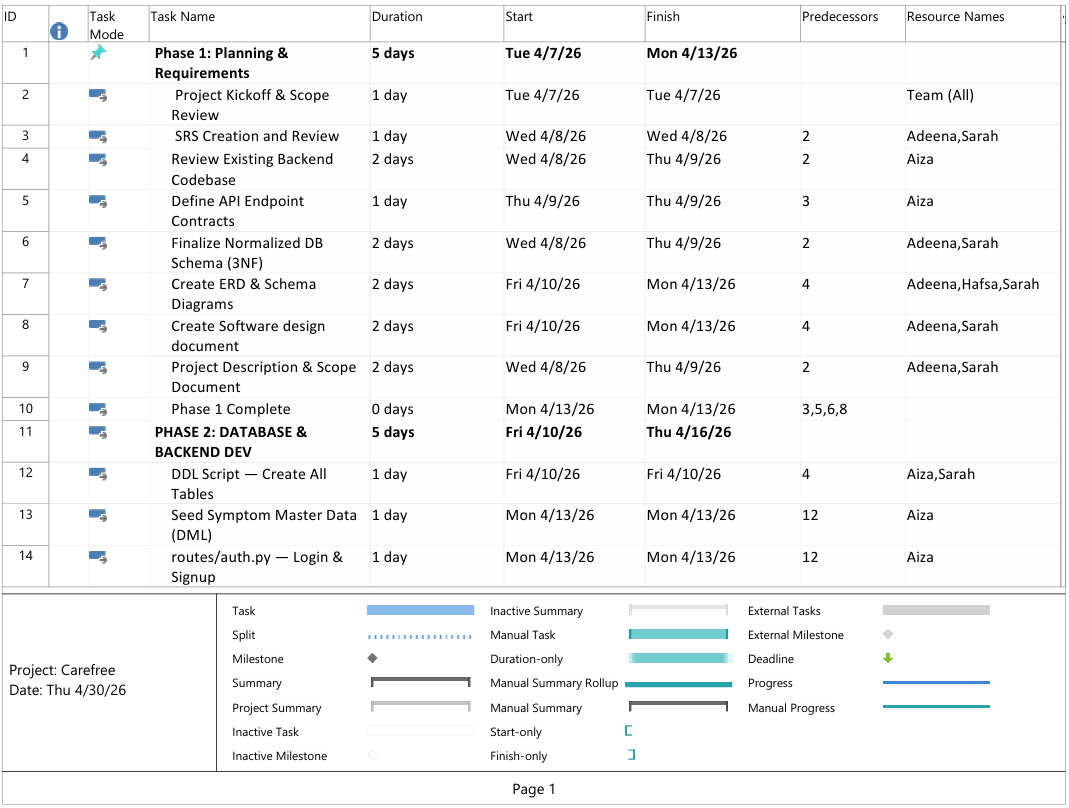
\includegraphics[width=0.75\textwidth]{project planning/planning_page1.png}
    \caption{Work Breakdown Structure}
\end{figure}
\begin{figure}[H]
    \centering
    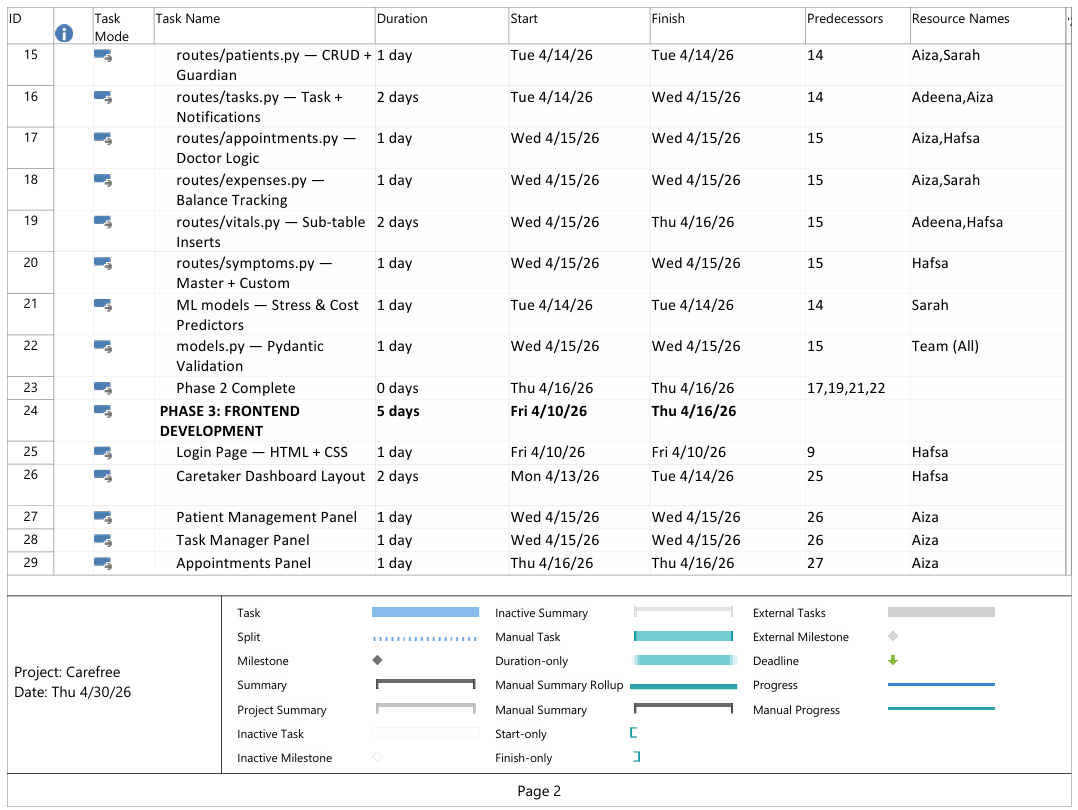
\includegraphics[width=0.85\textwidth]{project planning/planning_page2.png}
    \caption{Work Breakdown Structure: Continued}
\end{figure}
\begin{figure}[H]
    \centering
    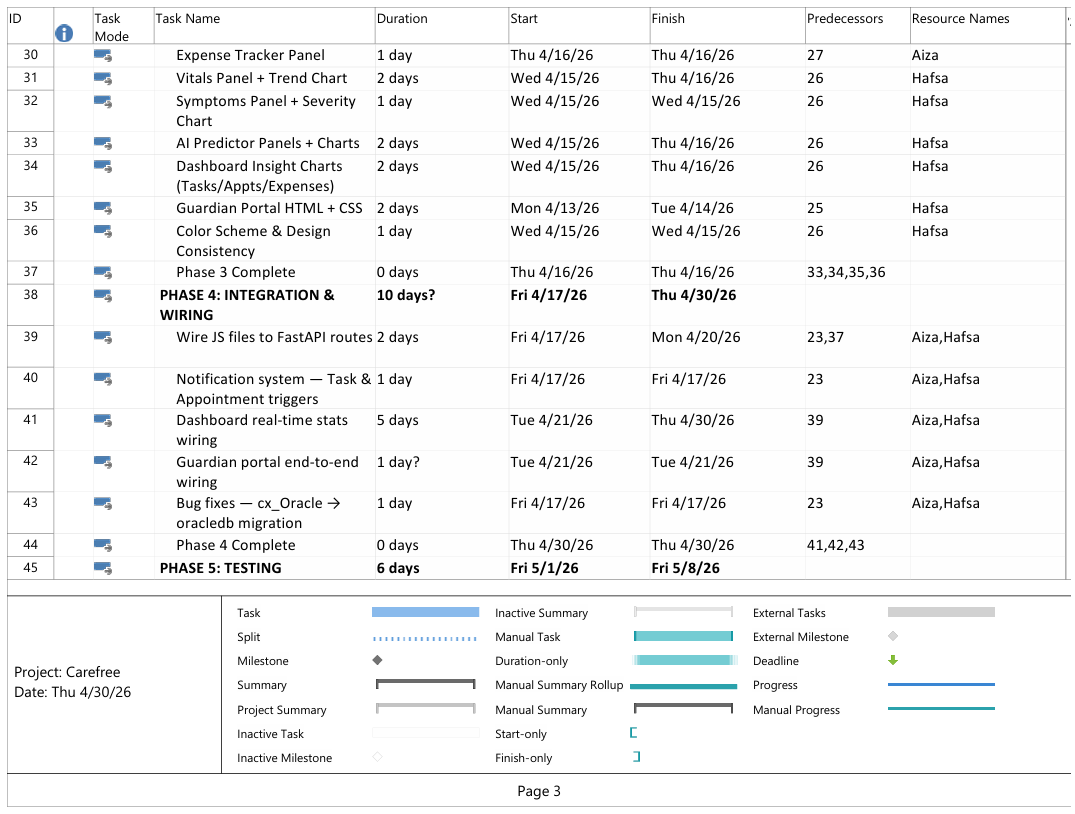
\includegraphics[width=0.85\textwidth]{project planning/planning_page3.png}
    \caption{Work Breakdown Structure: Continued}
\end{figure}
\begin{figure}[H]
    \centering
    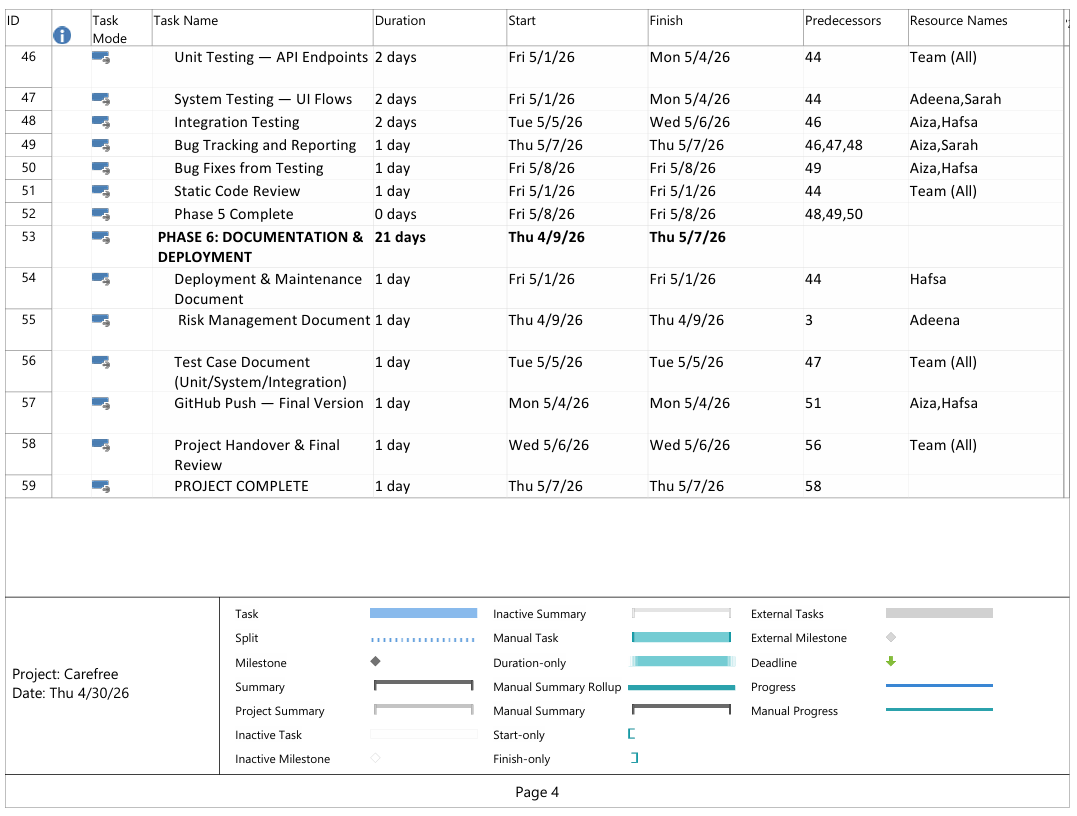
\includegraphics[width=0.85\textwidth]{project planning/planning_page4.png}
    \caption{Work Breakdown Structure: Continued}
\end{figure}
\subsection{Gantt Chart}
\begin{figure}[H]
    \centering
    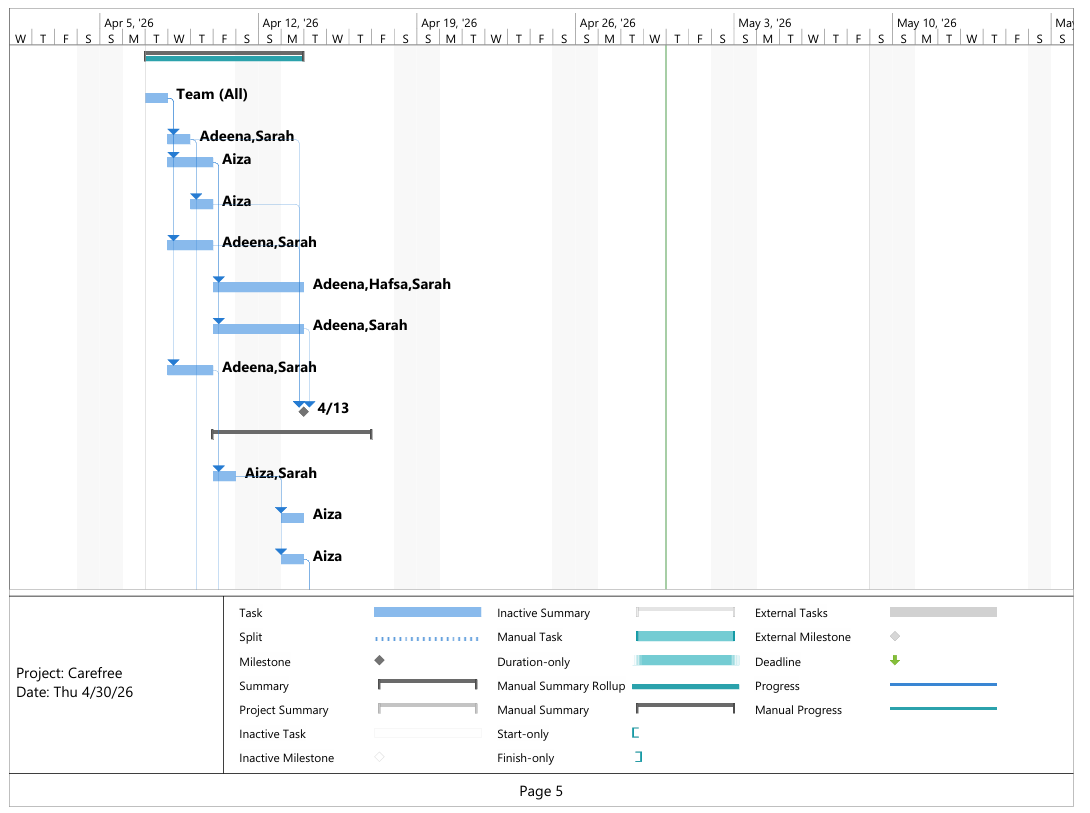
\includegraphics[width=0.75\textwidth]{project planning/planning_page5.png}
    \caption{Gantt Chart}
\end{figure}
\begin{figure}[H]
    \centering
    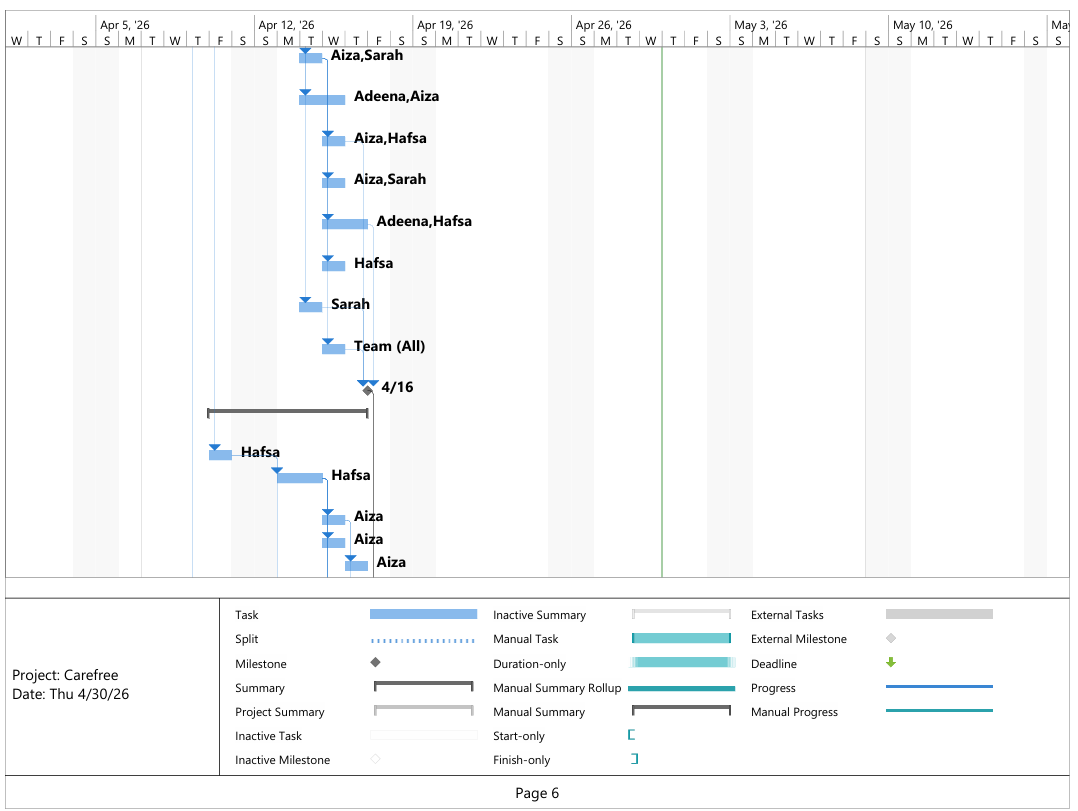
\includegraphics[width=0.85\textwidth]{project planning/planning_page6.png}
    \caption{Gantt Chart: Continued}
\end{figure}
\begin{figure}[H]
    \centering
    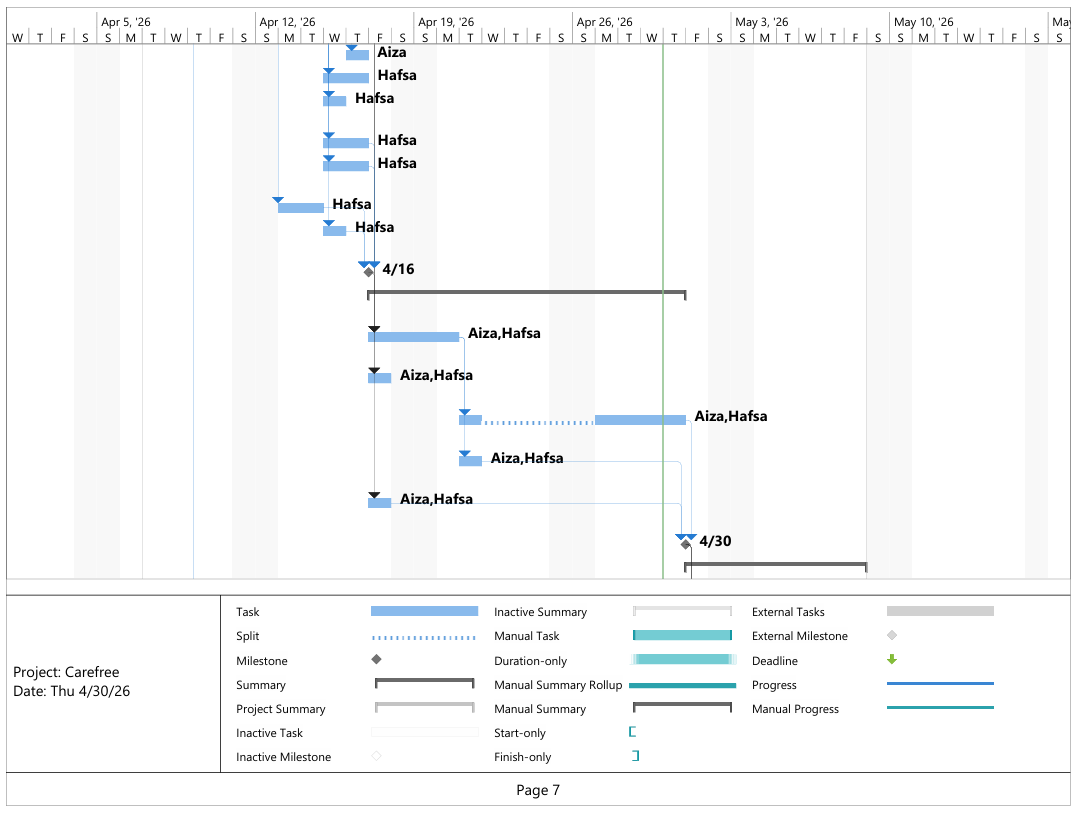
\includegraphics[width=0.85\textwidth]{project planning/planning_page7.png}
    \caption{Gantt Chart: Continued}
\end{figure}
\begin{figure}[H]
    \centering
    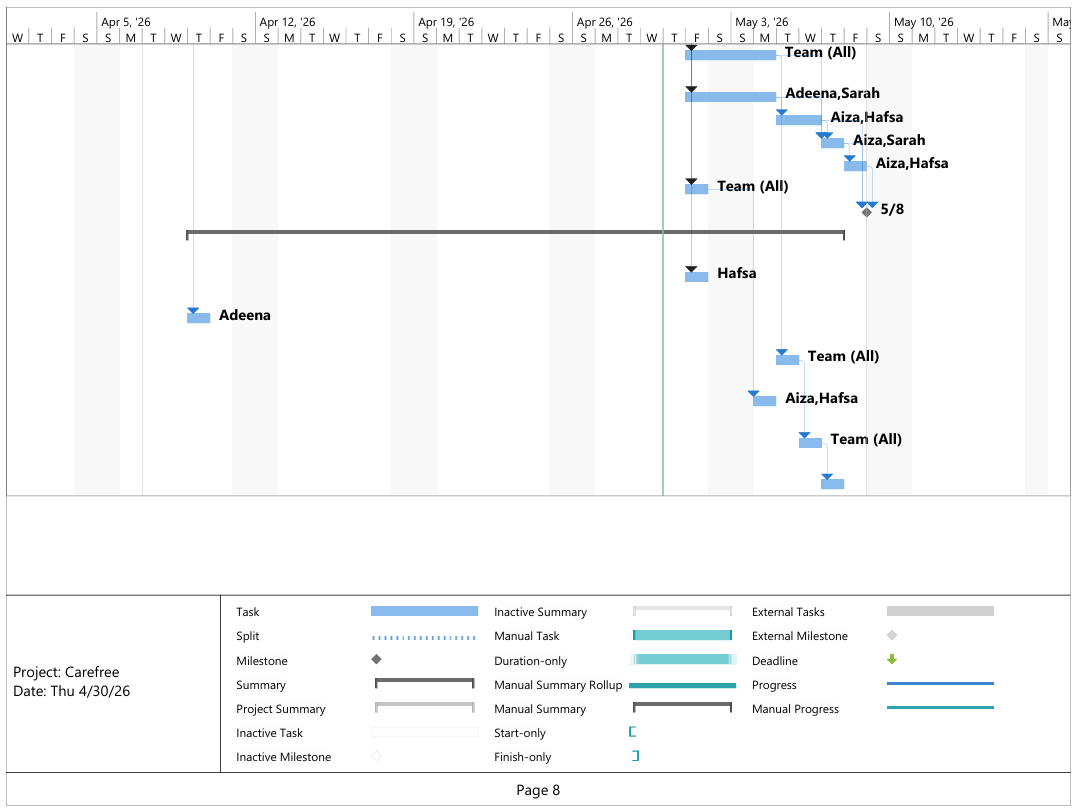
\includegraphics[width=0.85\textwidth]{project planning/planning_page8.png}
    \caption{Gantt Chart: Continued}
\end{figure}
\newpage
\subsection{Resource Sheet}
 
\begin{longtable}{|p{0.5cm}|p{2.5cm}|p{1cm}|p{3cm}|p{3.5cm}|p{2cm}|p{1.5cm}|}
    \hline
    \textbf{ID} & \textbf{Resource Name} & \textbf{Init.} & \textbf{Role} & \textbf{Responsibilities} & \textbf{Availability} & \textbf{Phase(s)} \\
    \hline
    \endfirsthead
    \hline
    \textbf{ID} & \textbf{Resource Name} & \textbf{Init.} & \textbf{Role} & \textbf{Responsibilities} & \textbf{Availability} & \textbf{Phase(s)} \\
    \hline
    \endhead
 
    1 & Sarah & S &
        Database Designer, ML Engineer, Software Designer and Architect &
        ERD/UML diagrams, DB normalisation, documentation and specifications, design document and requirement review, ML model training &
        Full-time (3 weeks) & 1, 2, 4, 5, 6 \\
    \hline
 
    2 & Adeena & A &
        Database Designer, Software Designer and Architect, Documentation &
        ERD/UML diagrams, DB normalisation, documentation and specifications, design document and requirement review, risk management &
        Full-time (3 weeks) & 1, 2, 4, 5, 6 \\
    \hline
 
    3 & Hafsa & H &
        Full Stack (Frontend Focused) Developer &
        HTML/CSS/JS for all panels, chart implementation, colour scheme, dashboard UI, guardian portal, deployment docs &
        Full-time (3 weeks) & 1, 3, 4, 5, 6 \\
    \hline
 
    4 & Aiza & A &
        Full Stack (Backend Focused) Developer / DBA &
        HTML/CSS/JS/PY for all panels, FastAPI routes, Oracle DDL/DML, DB creation, ML model integration, API contracts &
        Full-time (3 weeks) & 1, 2, 4, 5, 6 \\
    \hline
 
    5 & Team (All) & T &
        Full Team &
        Integration testing, bug fixes, project kickoff, API wiring, GitHub push, final review &
        Full-time (3 weeks) & 1, 4, 5, 6 \\
    \hline
 
    6 & Oracle XE 21c & O &
        Database System &
        Local relational database; hosts all patient, caretaker, guardian, task, appointment, vitals, and symptom data &
        Always-on (local machine) & All \\
    \hline
 
    7 & FastAPI + Uvicorn & F &
        Backend Framework &
        ASGI web server and REST API framework for all endpoints &
        Always-on (local machine) & All \\
    \hline
 
    8 & Chart.js CDN & C &
        Charting Library &
        All dashboard and predictor visualisations rendered client-side &
        On demand (browser) & 3, 4 \\
    \hline
 
    9 & scikit-learn & s &
        ML Framework &
        Stress level classification model and insurance cost regression model &
        Loaded at startup & 2, 4 \\
    \hline
 
    10 & GitHub & G &
        Version Control &
        Source code repository, collaboration between team members, deployment distribution &
        Always-on (cloud) & All \\
    \hline
 
\end{longtable}
\newpage

% ════════════════════════════════════════════════════════════════════════════
\section{Task 3 -- System Modeling}
% ════════════════════════════════════════════════════════════════════════════

\subsection{Use Case Diagram}

\begin{figure}[H]
    \centering
    \includegraphics[width=0.95\textwidth]{usecase.jpeg}
    \caption{Use Case Diagram}
\end{figure}

\subsection{Class Diagram}

\begin{figure}[H]
    \centering
    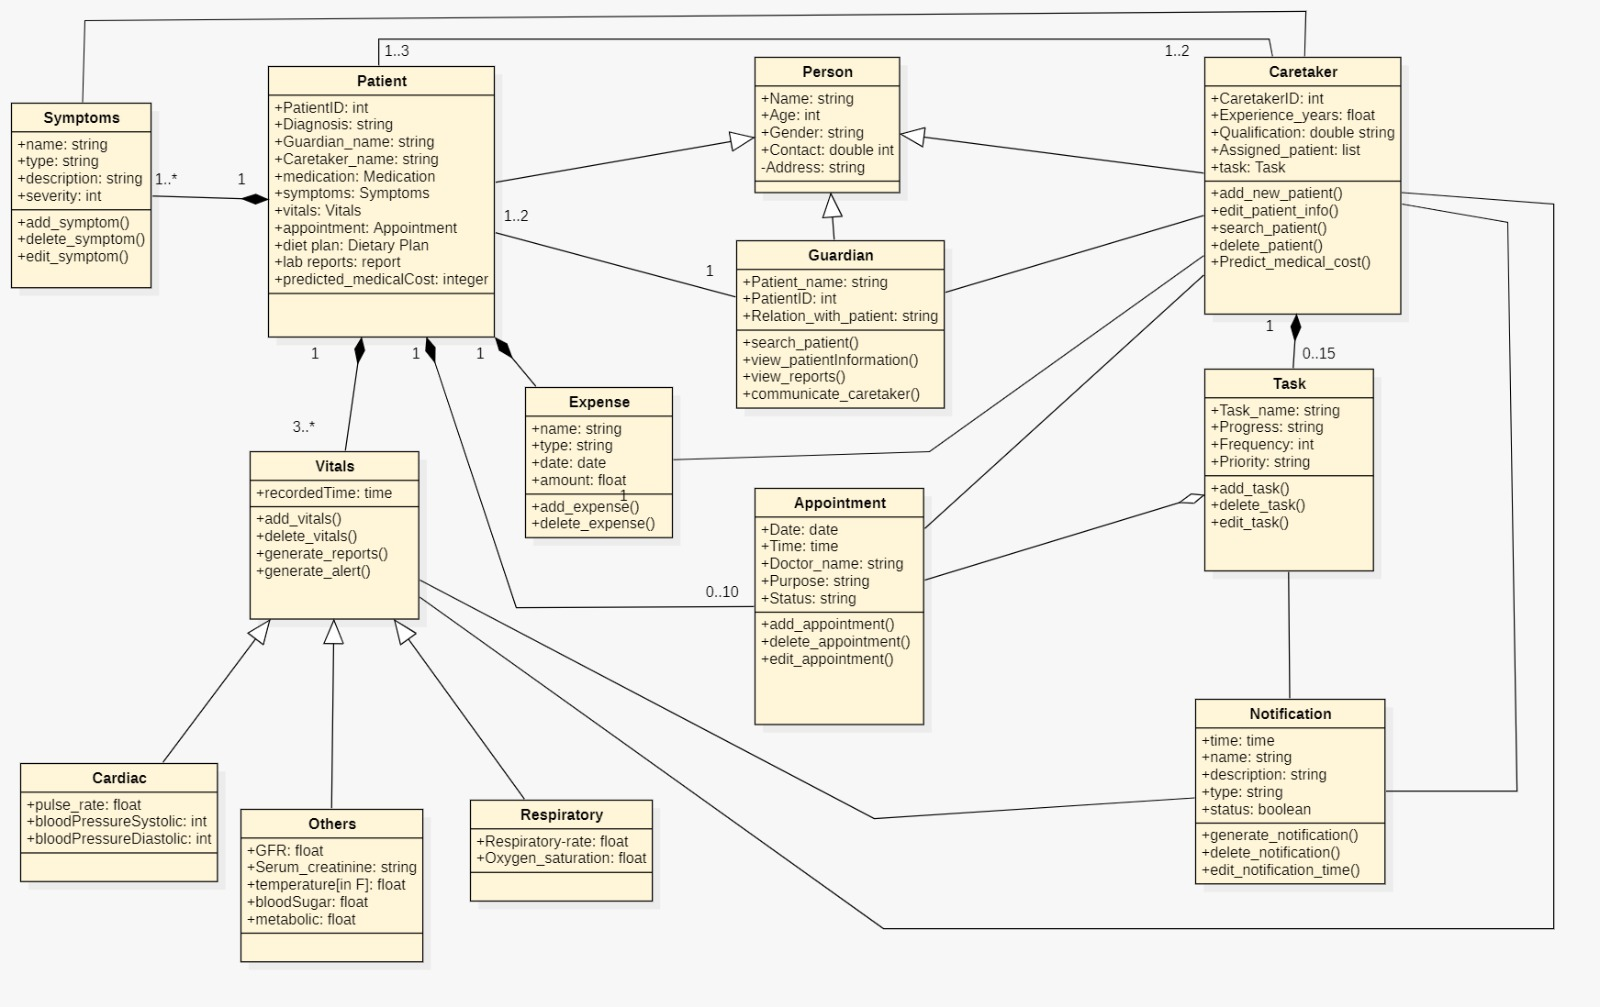
\includegraphics[width=1.05\textwidth]{images_scd_cea/class.jpeg}
    \caption{Class Diagram}
\end{figure}
\newpage
\subsection{Sequence Diagram}
The Sequence diagrams for this applications have been made feature wise that is each of the features has its own sequence diagrams.
\subsubsection{Login}

\begin{figure}[H]
    \centering
    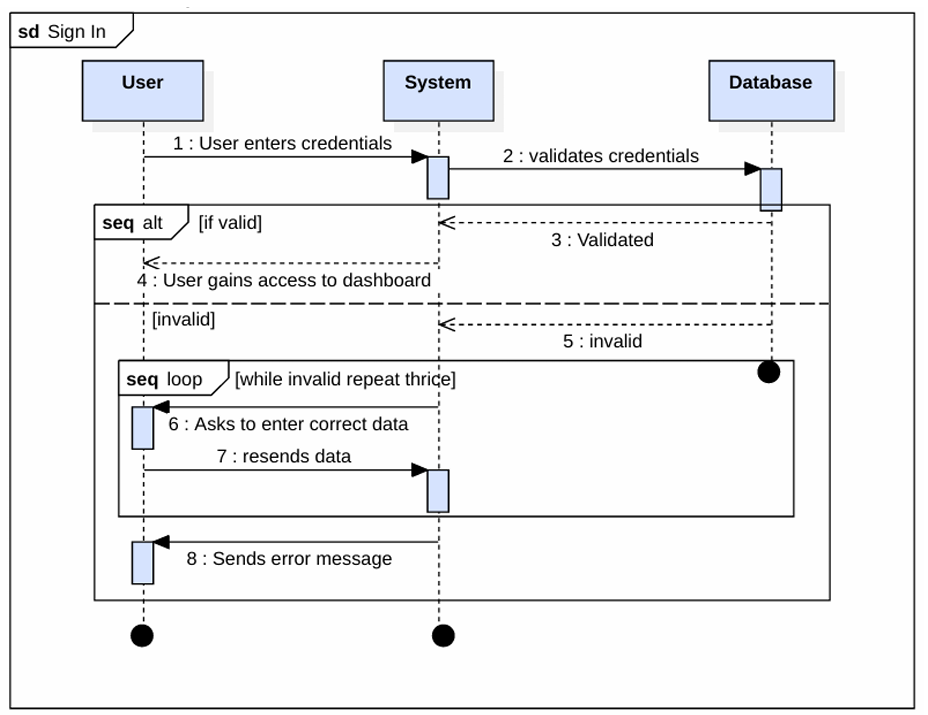
\includegraphics[width=0.75\textwidth]{images_scd_cea/sequence_signin.png}
    \caption{Sequence Diagram: Sign In}
\end{figure}

\subsubsection{Sign Up}
\begin{figure}[H]
    \centering
    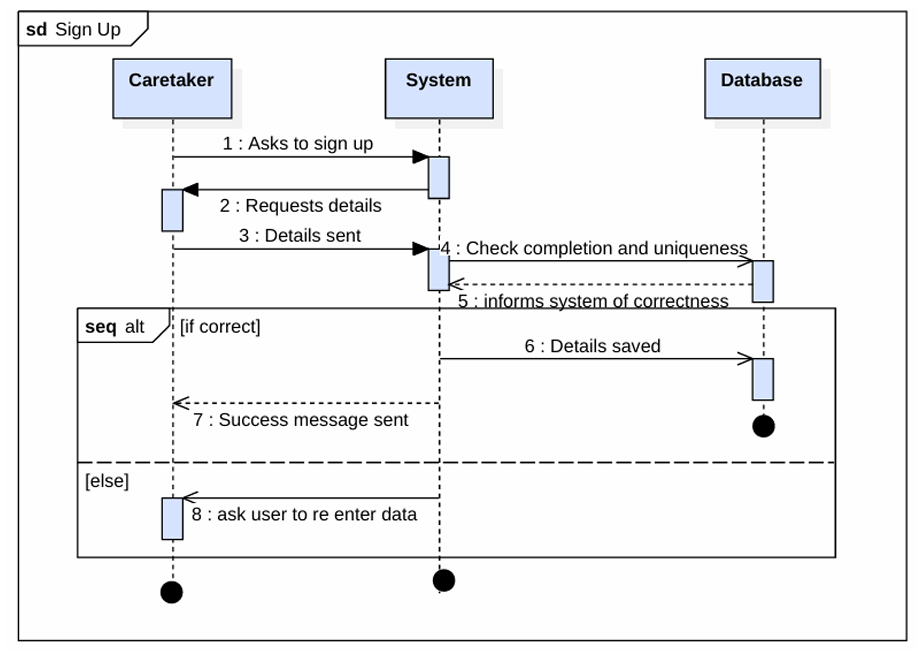
\includegraphics[width=0.75\textwidth]{images_scd_cea/sequence_signup.png}
    \caption{Sequence Diagram: Sign Up}
\end{figure}

\subsubsection{Sign Out}
\begin{figure}[H]
    \centering
    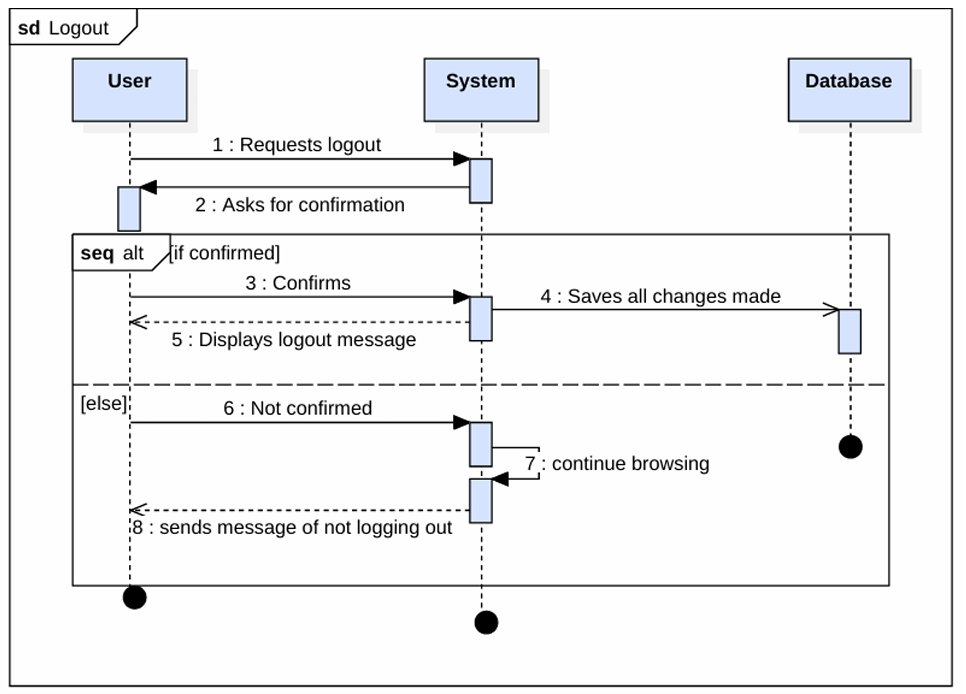
\includegraphics[width=0.75\textwidth]{images_scd_cea/sequence_signout.png}
    \caption{Sequence Diagram: Sign Out}
\end{figure}

\subsubsection{Patient Information Management}
\begin{figure}[H]
    \centering
    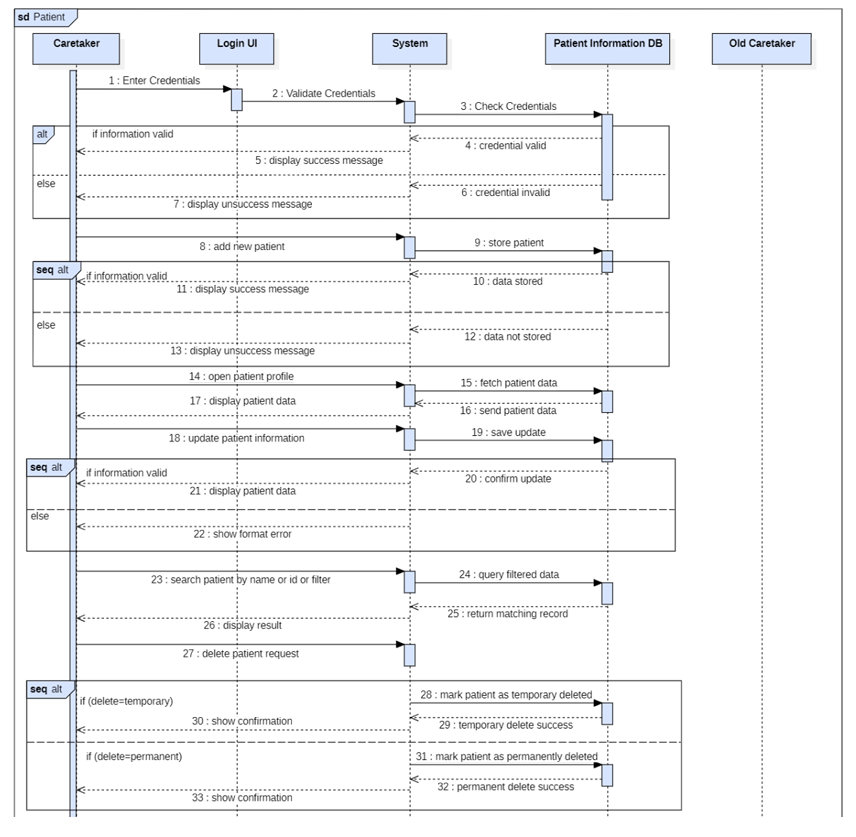
\includegraphics[width=1.05\textwidth]{images_scd_cea/sequence_pt_mgmt1.png}
\end{figure}
\begin{figure}[H]
    \centering
    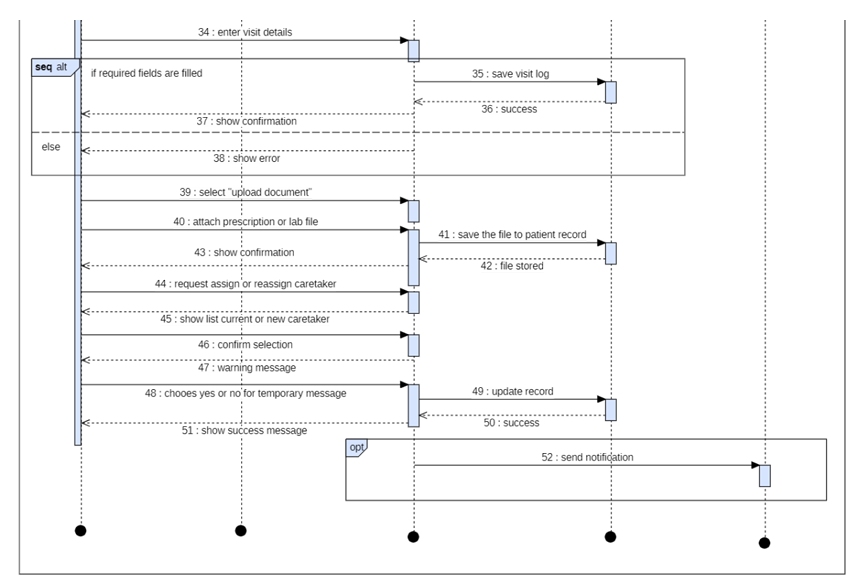
\includegraphics[width=1.05\textwidth]{images_scd_cea/sequence_pt_mgmt2.png}
    \caption{Sequence Diagram: Patient Information Management}
\end{figure}

\subsubsection{Appointment Tracking}
\begin{figure}[H]
    \centering
    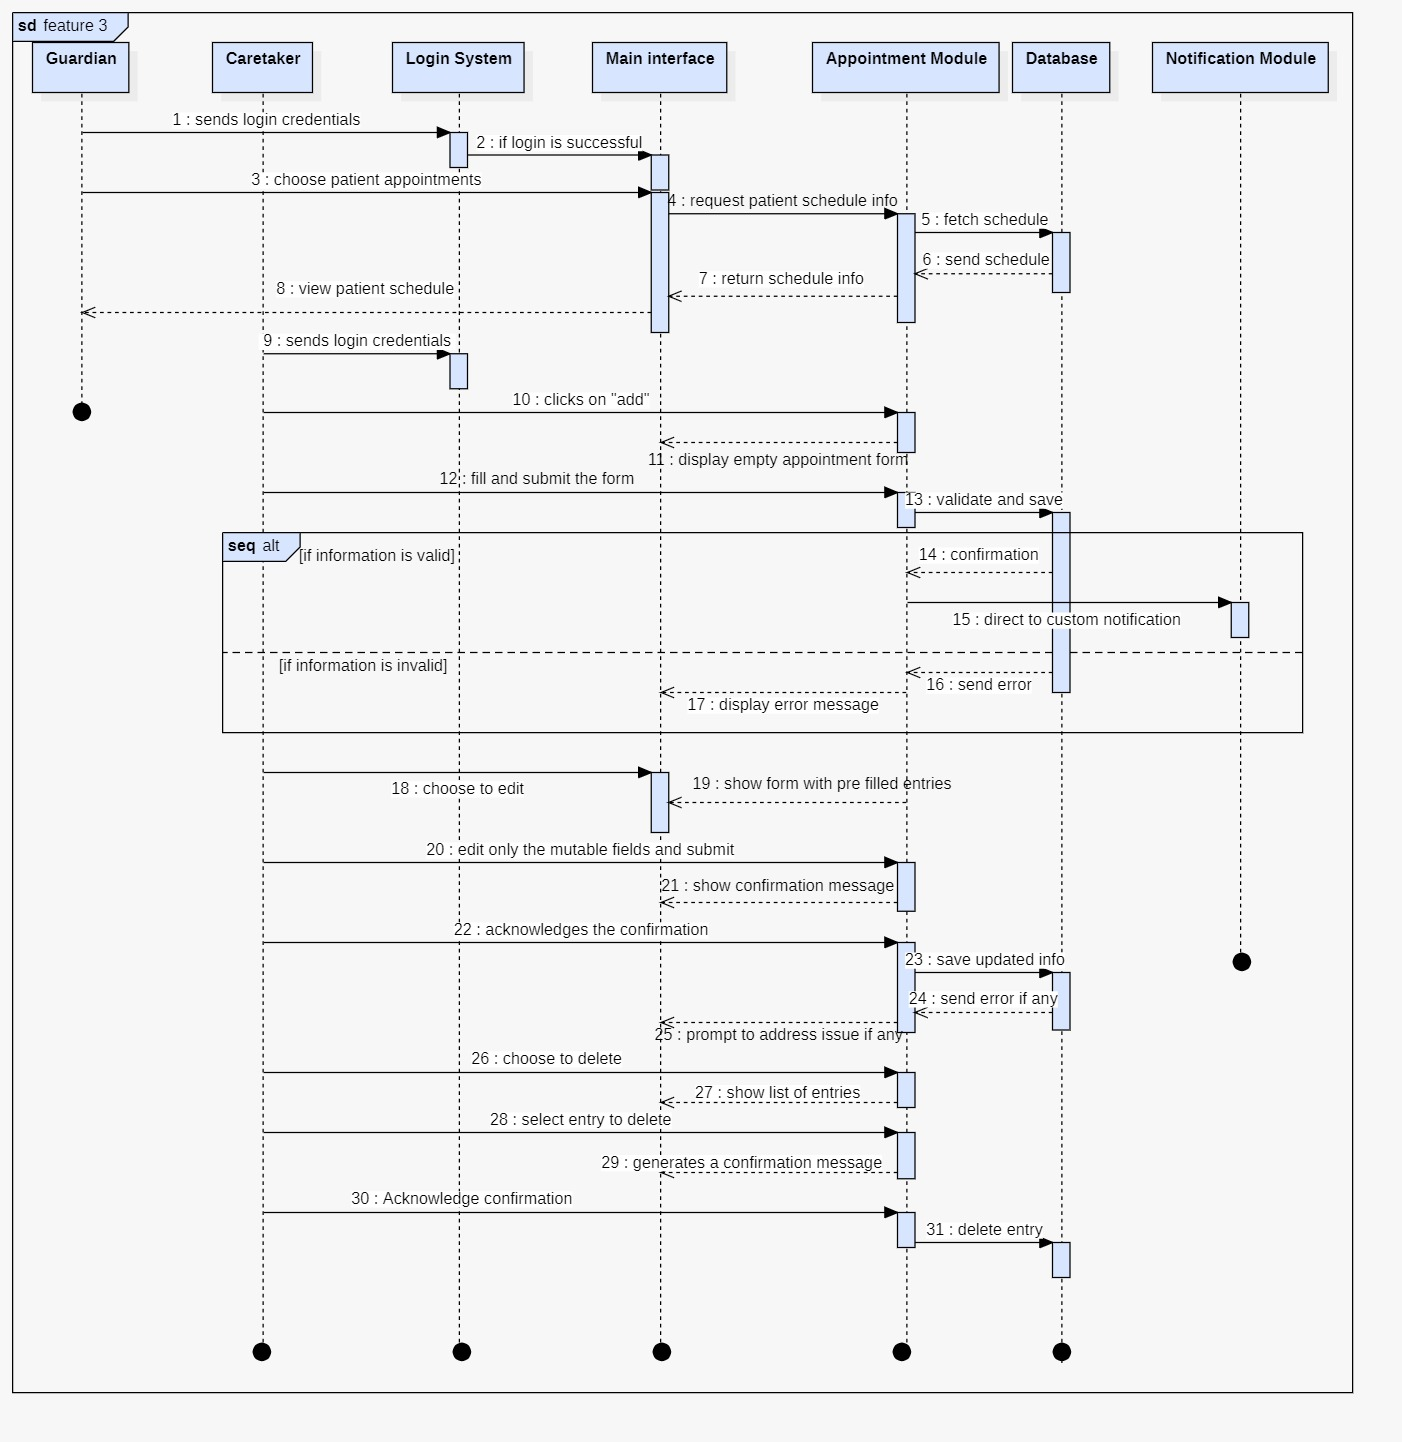
\includegraphics[width=0.95\textwidth]{images_scd_cea/sequence_appt.jpeg}
    \caption{Sequence Diagram}
\end{figure}

\subsubsection{Caretaker Task Management}
\begin{figure}[H]
    \centering
    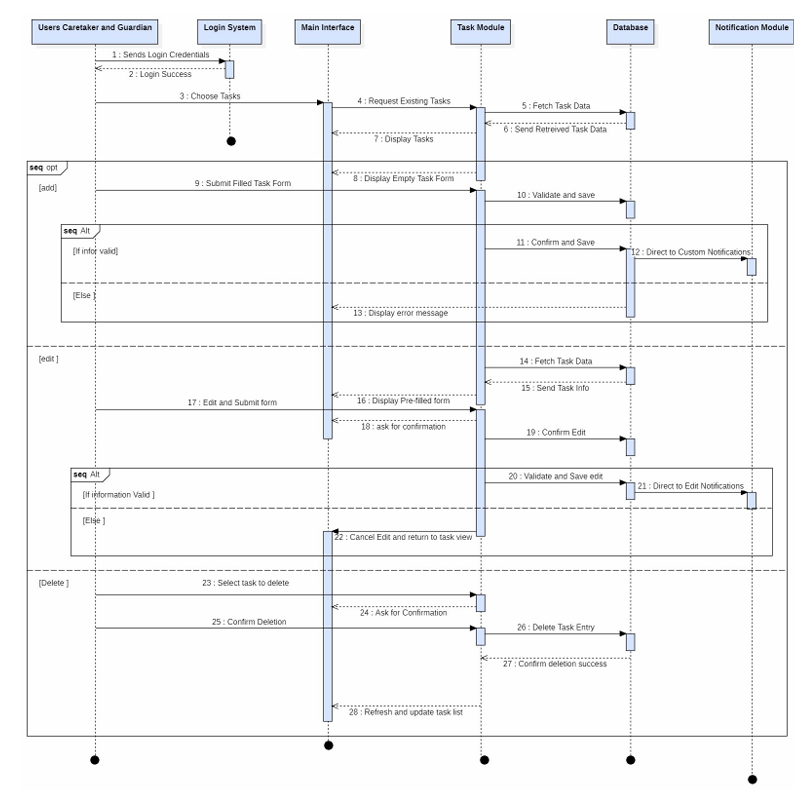
\includegraphics[width=1.05\textwidth]{images_scd_cea/sequence_task.png}
    \caption{Sequence Diagram: Caretaker Task Management}
\end{figure}

\subsubsection{Expense Tracker}
\begin{figure}[H]
    \centering
    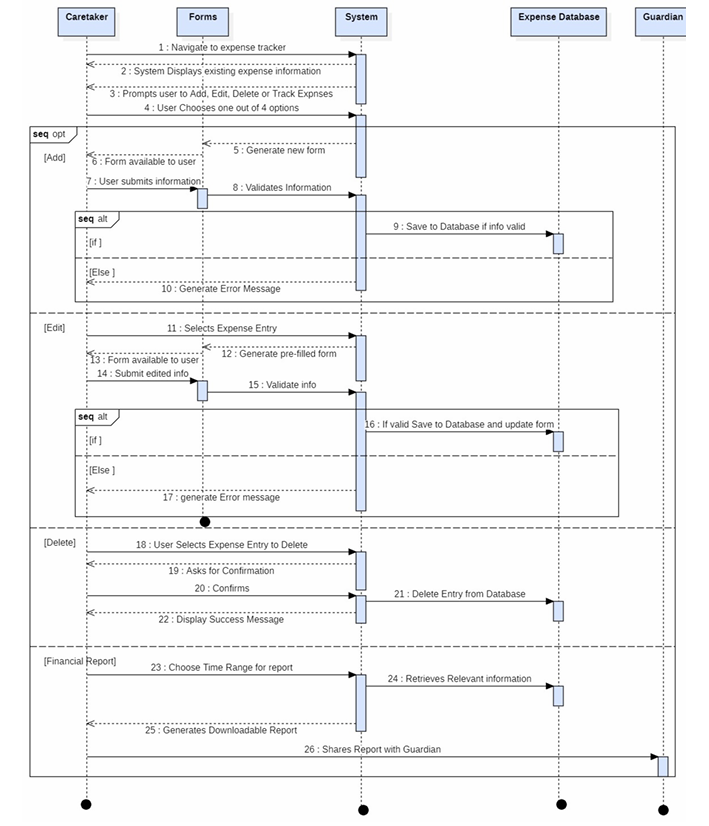
\includegraphics[width=0.95\textwidth]{images_scd_cea/sequence_expense.png}
    \caption{Sequence Diagram: Expense Tracker}
\end{figure}

\subsubsection{Notifications}
\begin{figure}[H]
    \centering
    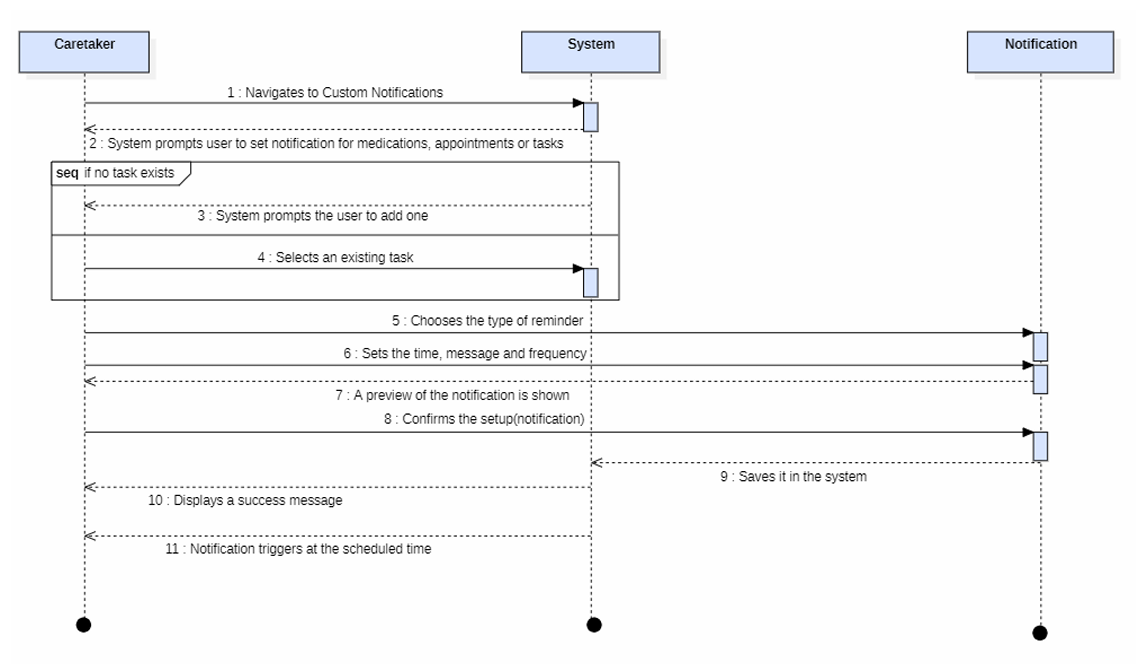
\includegraphics[width=0.95\textwidth]{images_scd_cea/sequence_notification.png}
    \caption{Sequence Diagram: Notifications}
\end{figure}

\subsubsection{ML Medical Cost predictor}
\begin{figure}[H]
    \centering
    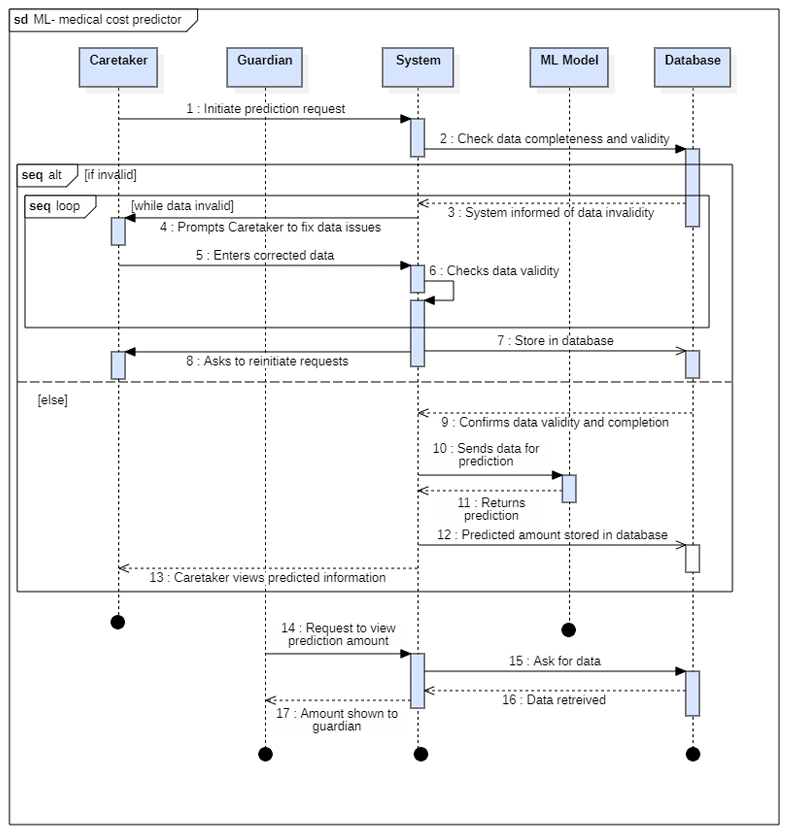
\includegraphics[width=0.75\textwidth]{images_scd_cea/sequence_cost.png}
    \caption{Sequence Diagram: ML medical Cost Predictor}
\end{figure}

\subsubsection{ML Stress Classifier}
\begin{figure}[H]
    \centering
    \includegraphics[width=0.75\textwidth]{ML- stress predictor.png}
    \caption{Sequence Diagram: ML Stress Classifier}
\end{figure}

\subsubsection{Vitals and Symptoms Tracker}
\begin{figure}[H]
    \centering
    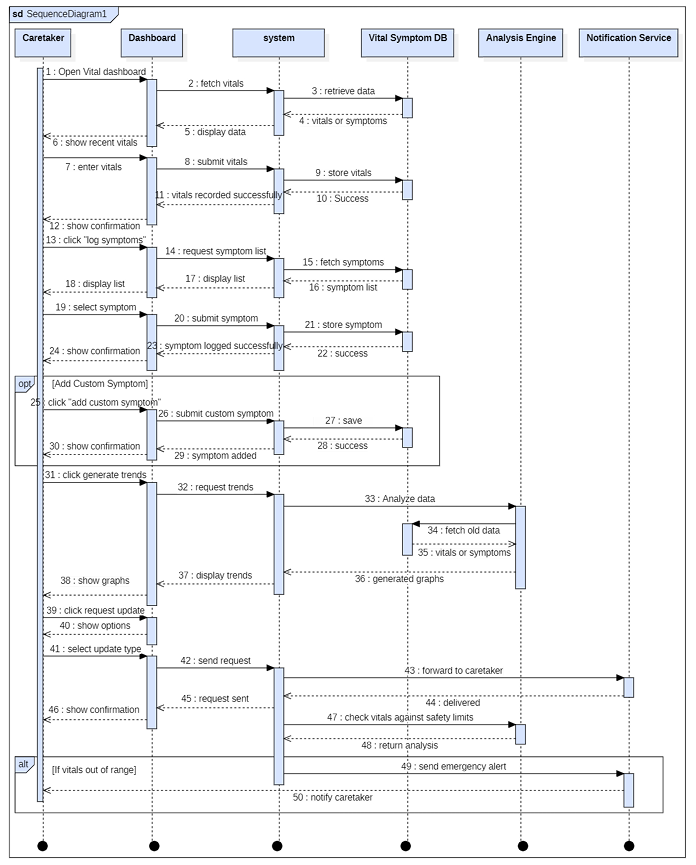
\includegraphics[width=0.95\textwidth]{images_scd_cea/sequence_vitals.png}
    \caption{Sequence Diagram: Vitals and Symptoms Tracker}
\end{figure}

\newpage
\subsection{State Chart Diagram}
The State diagrams for this applications have been made feature wise that is each of the features has its own state diagrams.
\subsubsection{Login}

\begin{figure}[H]
    \centering
    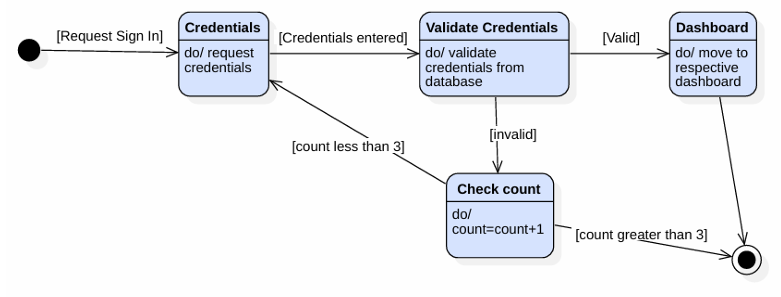
\includegraphics[width=0.75\textwidth]{images_scd_cea/state_signup.png}
    \caption{State Diagram: Sign In}
\end{figure}

\subsubsection{Sign Up}
\begin{figure}[H]
    \centering
    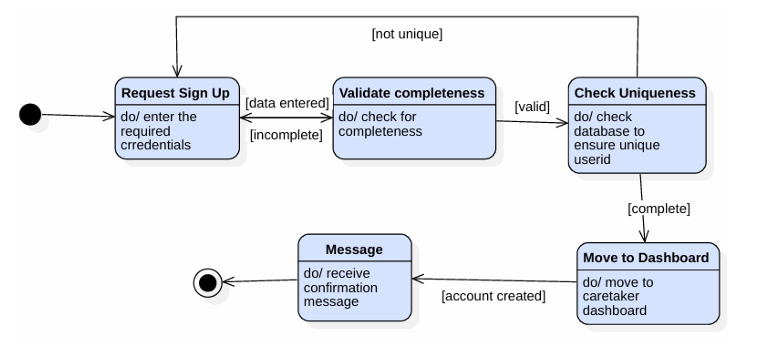
\includegraphics[width=0.75\textwidth]{images_scd_cea/state_signin.png}
    \caption{State Diagram: Sign Up}
\end{figure}

\subsubsection{Sign Out}
\begin{figure}[H]
    \centering
    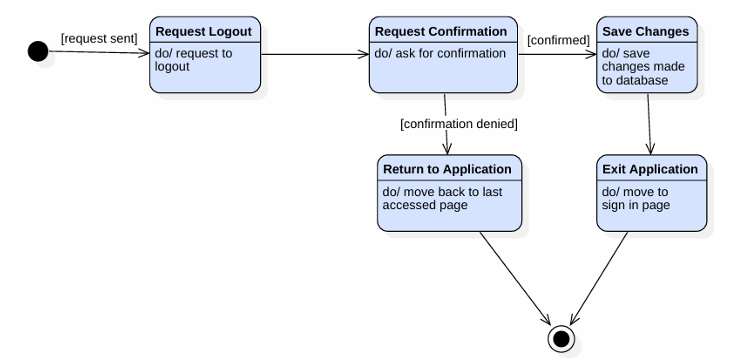
\includegraphics[width=0.75\textwidth]{images_scd_cea/state_sigout.png}
    \caption{State Diagram: Sign Out}
\end{figure}

\subsubsection{Patient Information Management}
\begin{figure}[H]
    \centering
    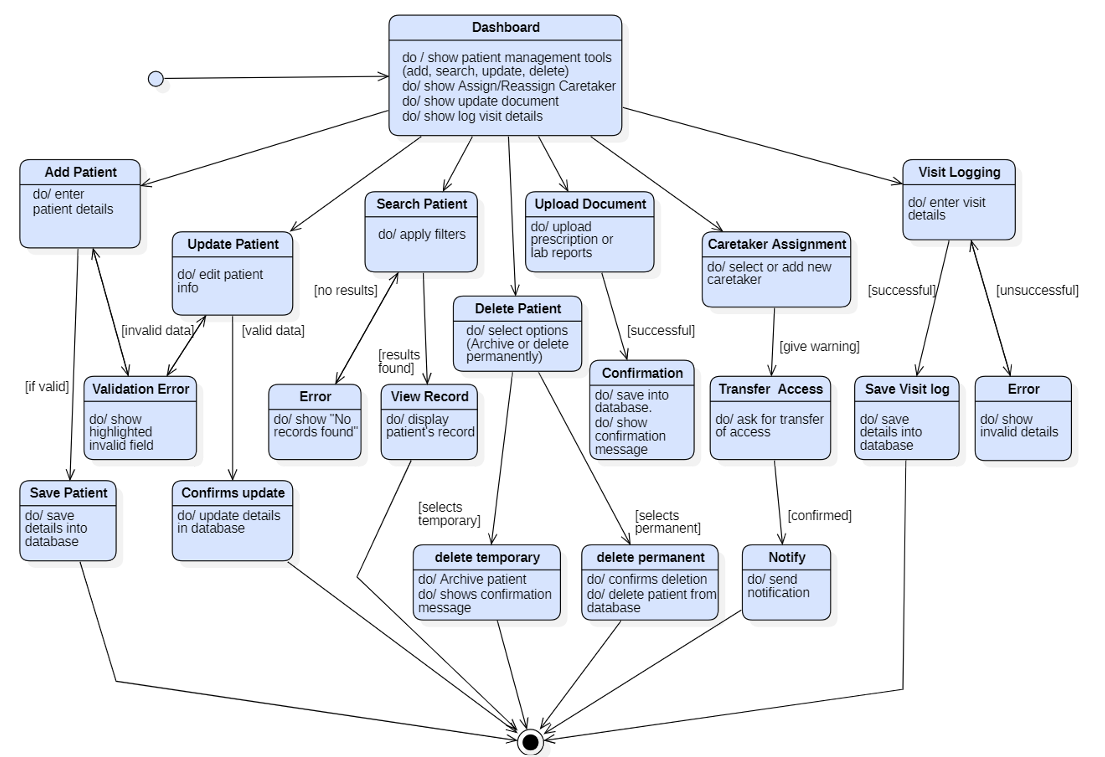
\includegraphics[width=1.05\textwidth]{images_scd_cea/state_ptmgmt.png}
    \caption{State Diagram: Patient Information Management}
\end{figure}

\subsubsection{Appointment Tracking}
\begin{figure}[H]
    \centering
    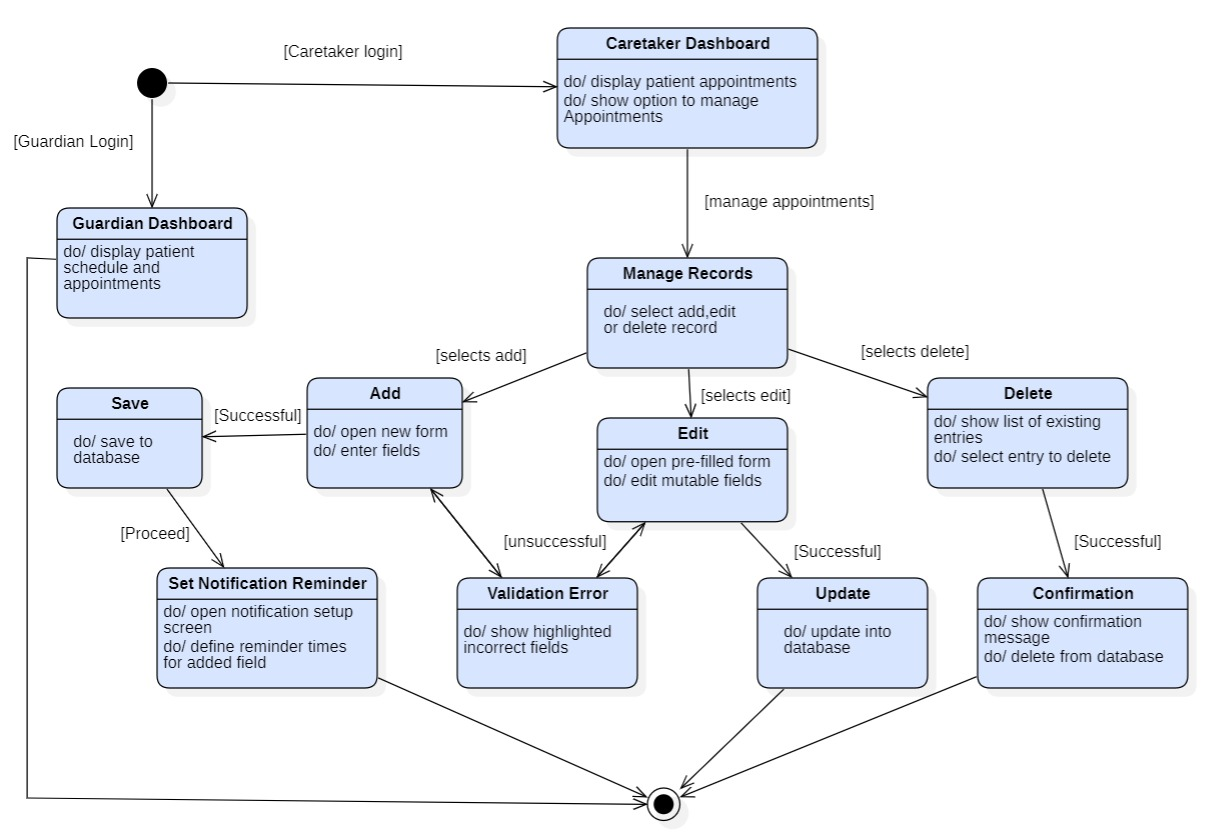
\includegraphics[width=0.75\textwidth]{images_scd_cea/state_appt.jpeg}
    \caption{State Diagram: Appointment Tracking}
\end{figure}

\subsubsection{Caretaker Task Management}
\begin{figure}[H]
    \centering
    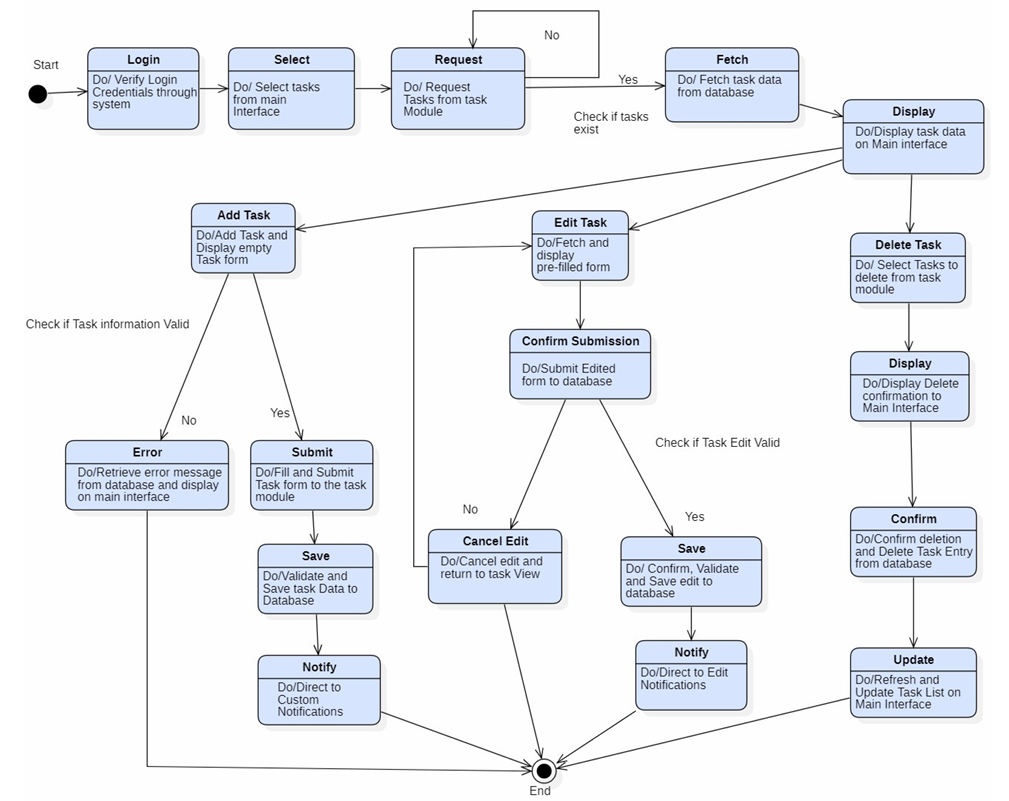
\includegraphics[width=1.05\textwidth]{images_scd_cea/state_task.png}
    \caption{State Diagram: Caretaker Task Management}
\end{figure}

\subsubsection{Expense Tracker}
\begin{figure}[H]
    \centering
    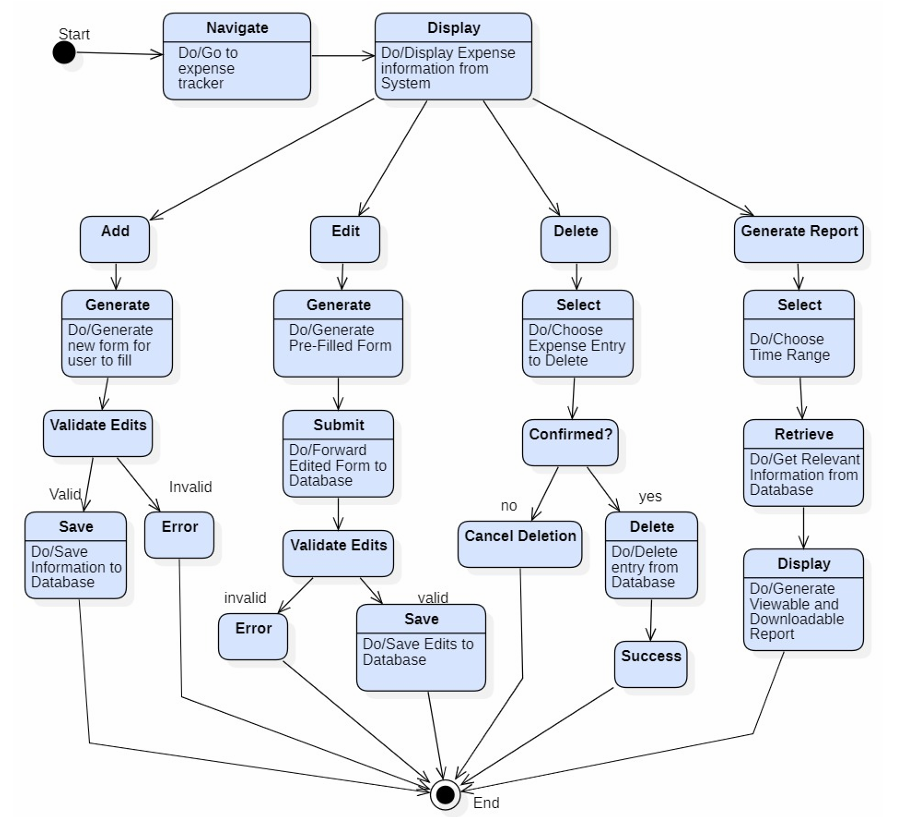
\includegraphics[width=0.95\textwidth]{images_scd_cea/state_expense.png}
    \caption{State Diagram: Expense Tracker}
\end{figure}

\subsubsection{Notifications}
\begin{figure}[H]
    \centering
    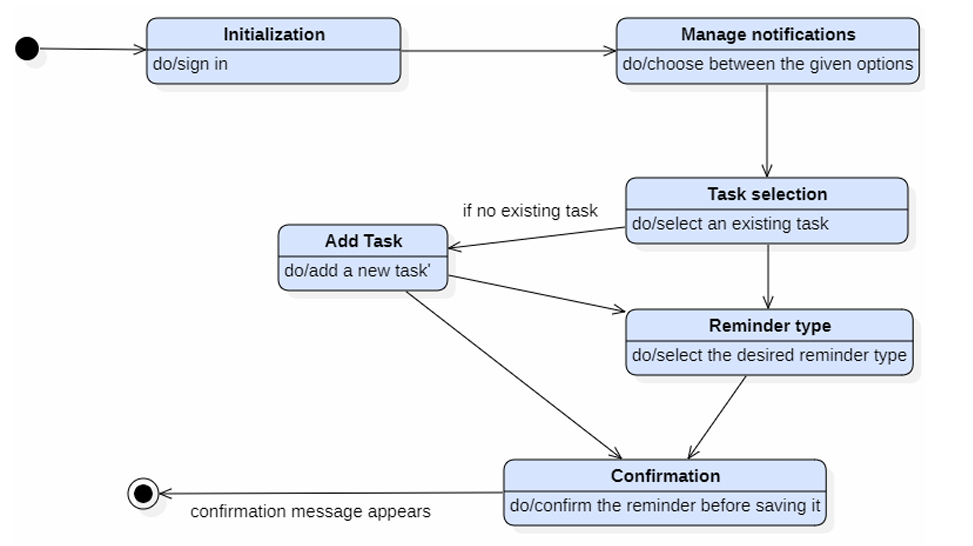
\includegraphics[width=0.95\textwidth]{images_scd_cea/state_notification.png}
    \caption{State Diagram: Notifications}
\end{figure}

\subsubsection{ML Medical Cost predictor}
\begin{figure}[H]
    \centering
    \includegraphics[width=0.75\textwidth]{ML-costpredictor-state.png}
    \caption{State Diagram: ML medical Cost Predictor}
\end{figure}

\subsubsection{ML Stress Classifier}
\begin{figure}[H]
    \centering
    \includegraphics[width=0.75\textwidth]{state-MLstress predictor.png}
    \caption{State Diagram: ML Stress Classifier}
\end{figure}

\subsubsection{Vitals and Symptoms Tracker}
\begin{figure}[H]
    \centering
    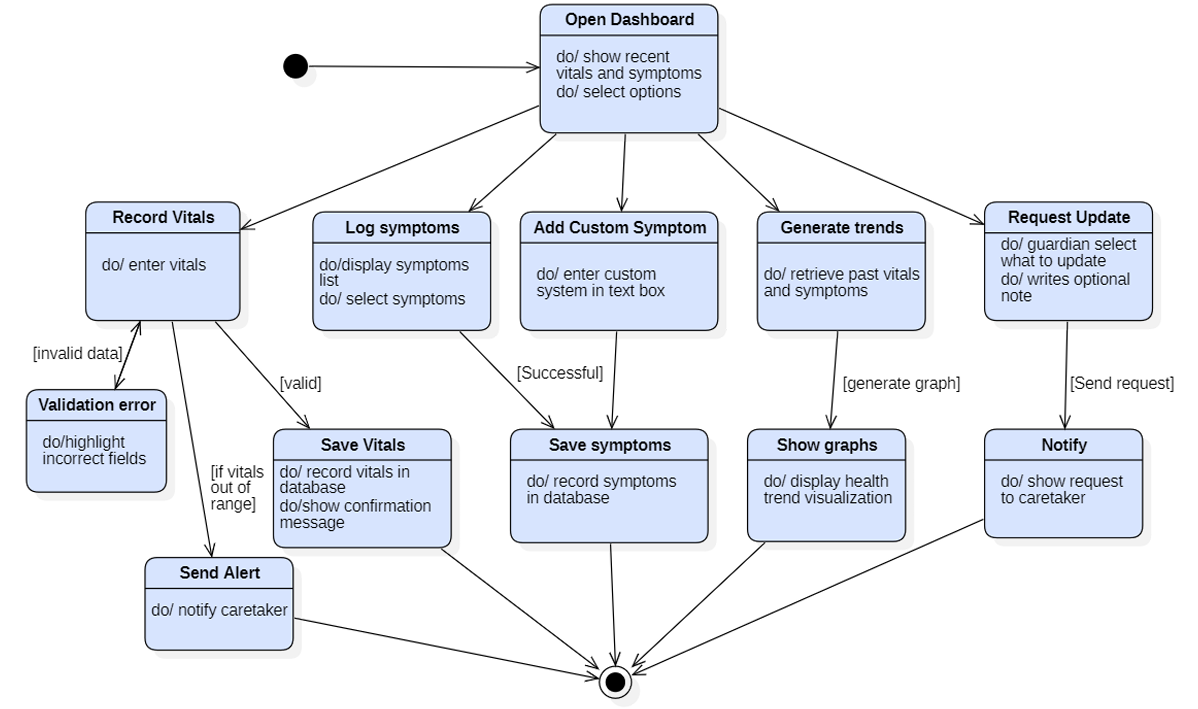
\includegraphics[width=1\textwidth]{images_scd_cea/state_vitals.png}
    \caption{State Diagram: Vitals and SYmptoms Tracker}
\end{figure}

\newpage

% ════════════════════════════════════════════════════════════════════════════
\section{Task 4 -- System Development}

\subsection{External Schema}
\subsubsection{Login and Sign Up}
\begin{figure}[H]
    \centering
    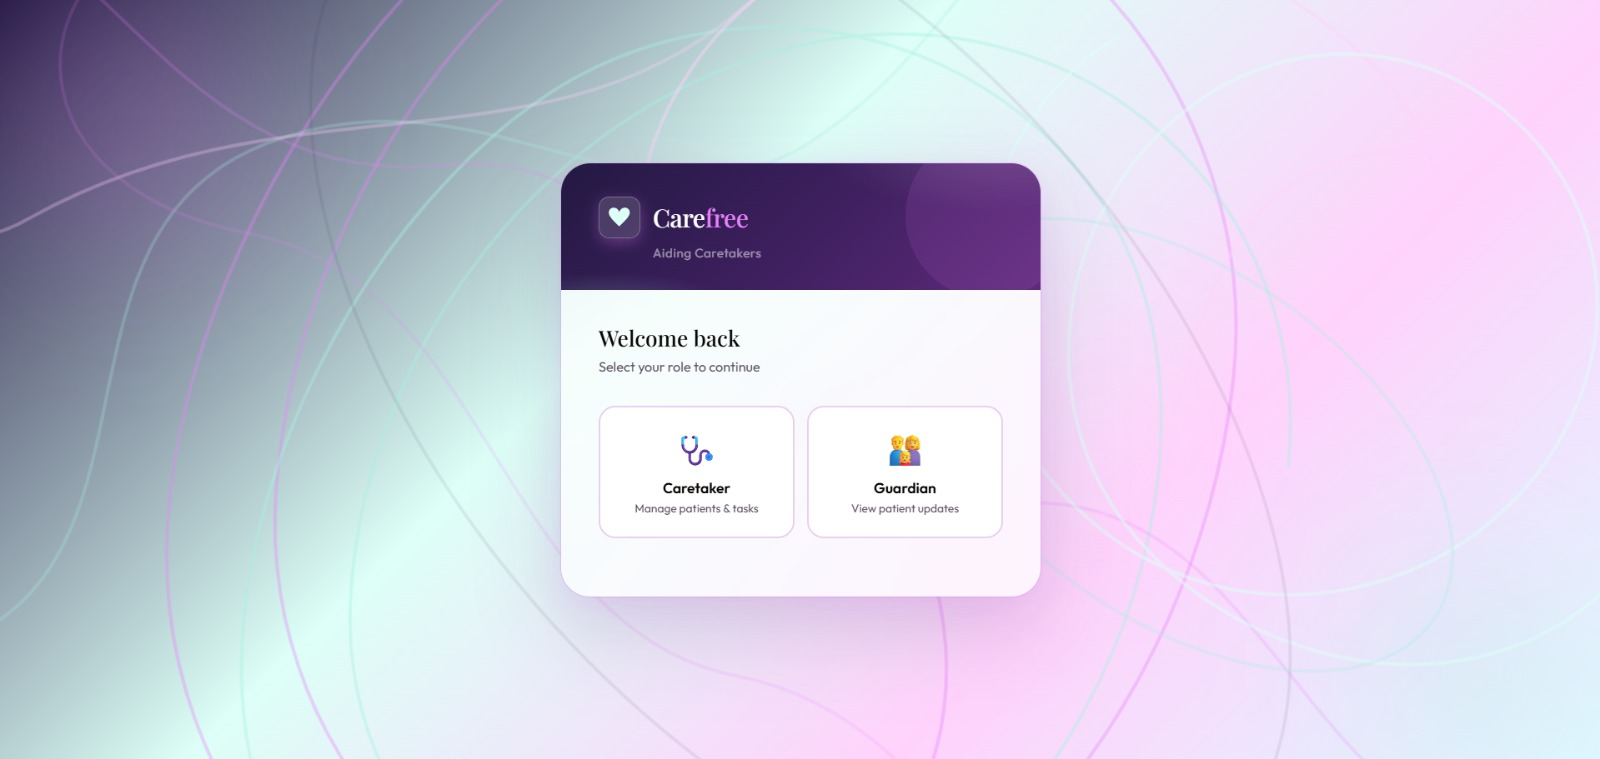
\includegraphics[width=0.85\textwidth]{external_schema/sign_up_login1.jpeg}
    \caption{Choose your Role}
\end{figure}
\begin{figure}[H]
    \centering
    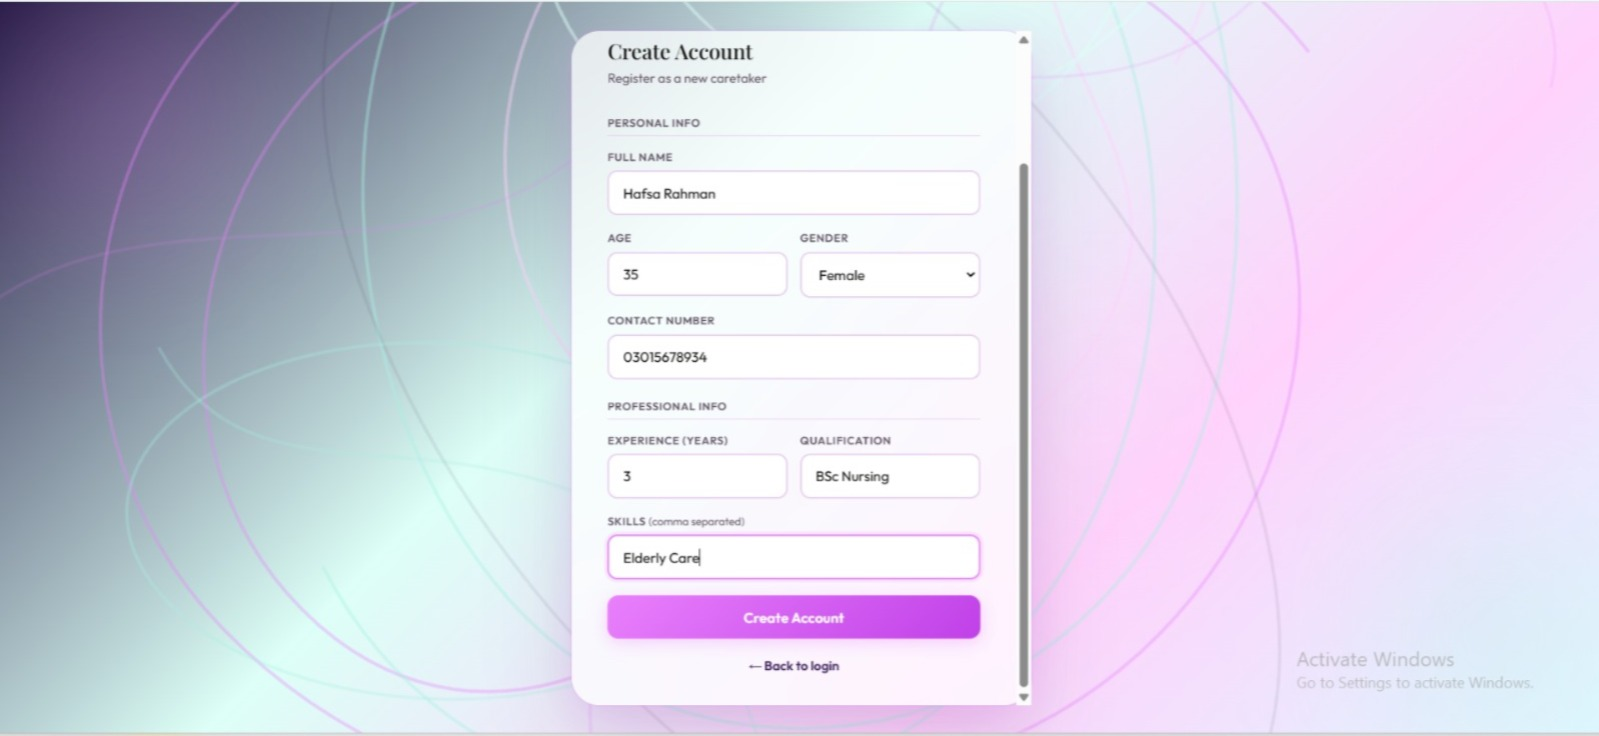
\includegraphics[width=0.85\textwidth]{external_schema/caretaker_signup2.jpeg}
    \caption{Caretaker sign Up}
\end{figure}
\begin{figure}[H]
    \centering
    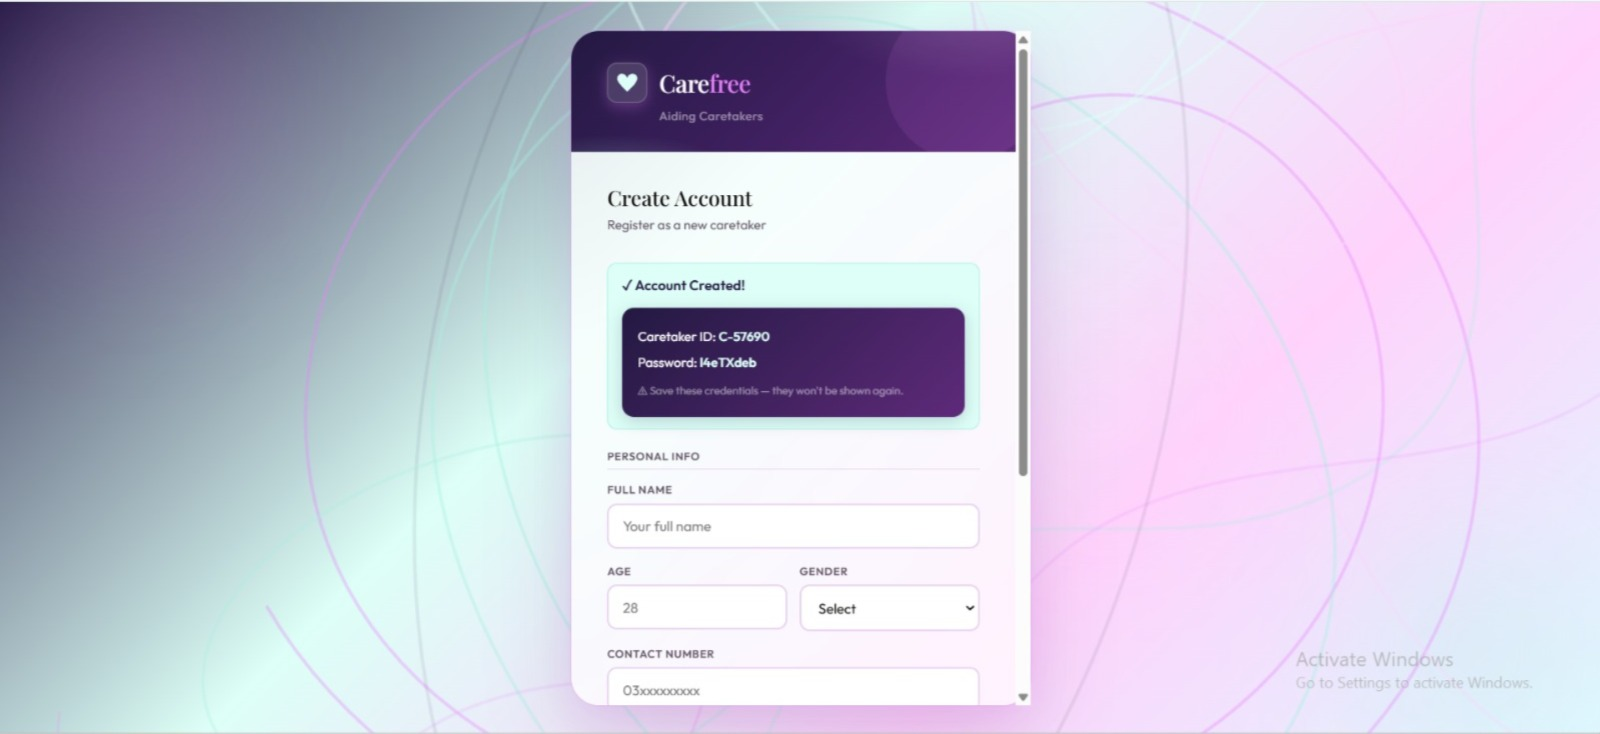
\includegraphics[width=0.85\textwidth]{external_schema/caretaker_signup1.jpeg}
    \caption{Caretaker Sign Up: Continued}
\end{figure}
\begin{figure}[H]
    \centering
    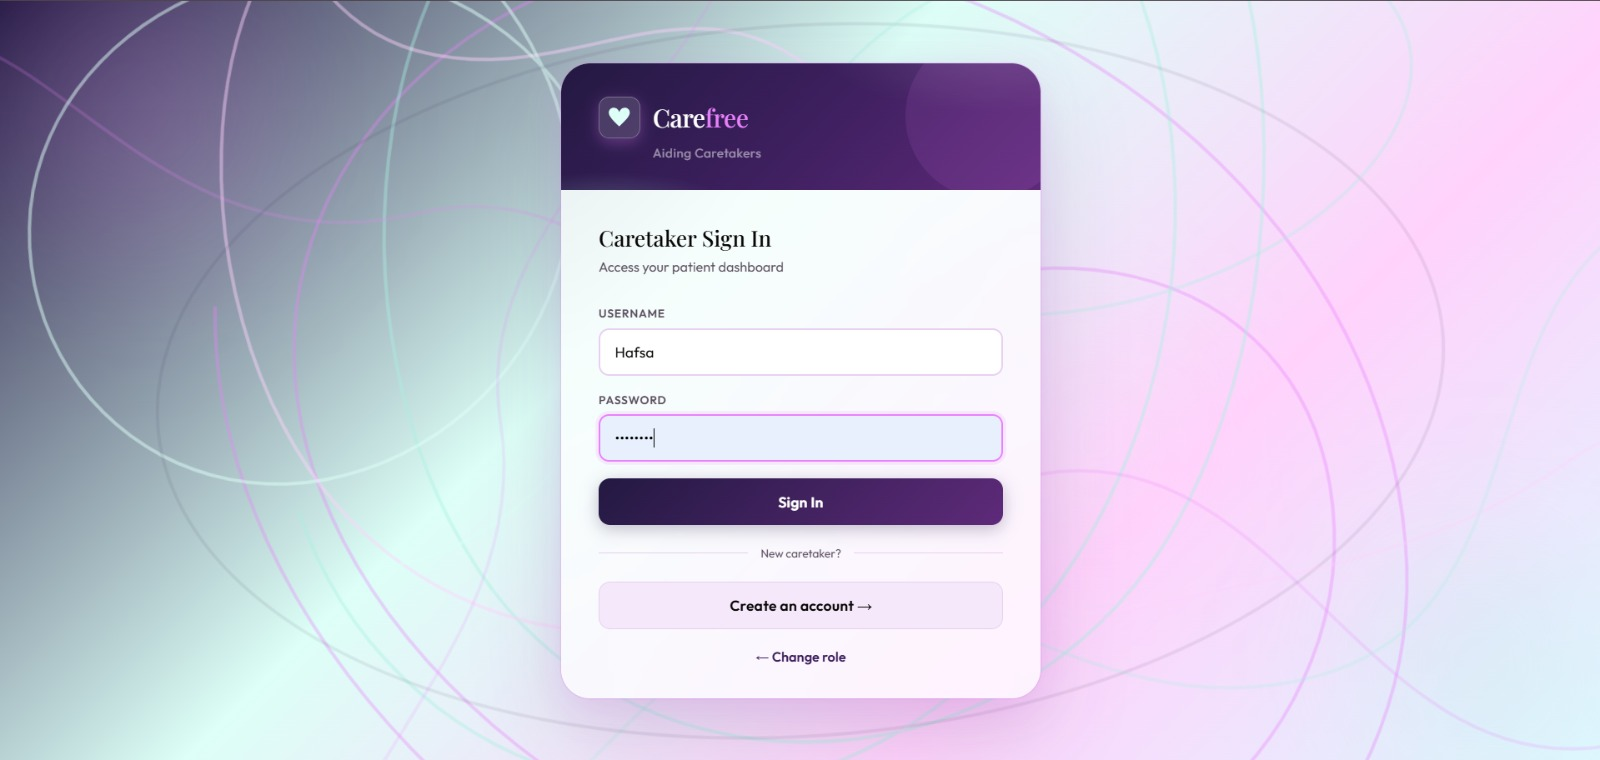
\includegraphics[width=0.85\textwidth]{external_schema/caretaker_signin.jpeg}
    \caption{Caretaker Sign In}
\end{figure}
\begin{figure}[H]
    \centering
    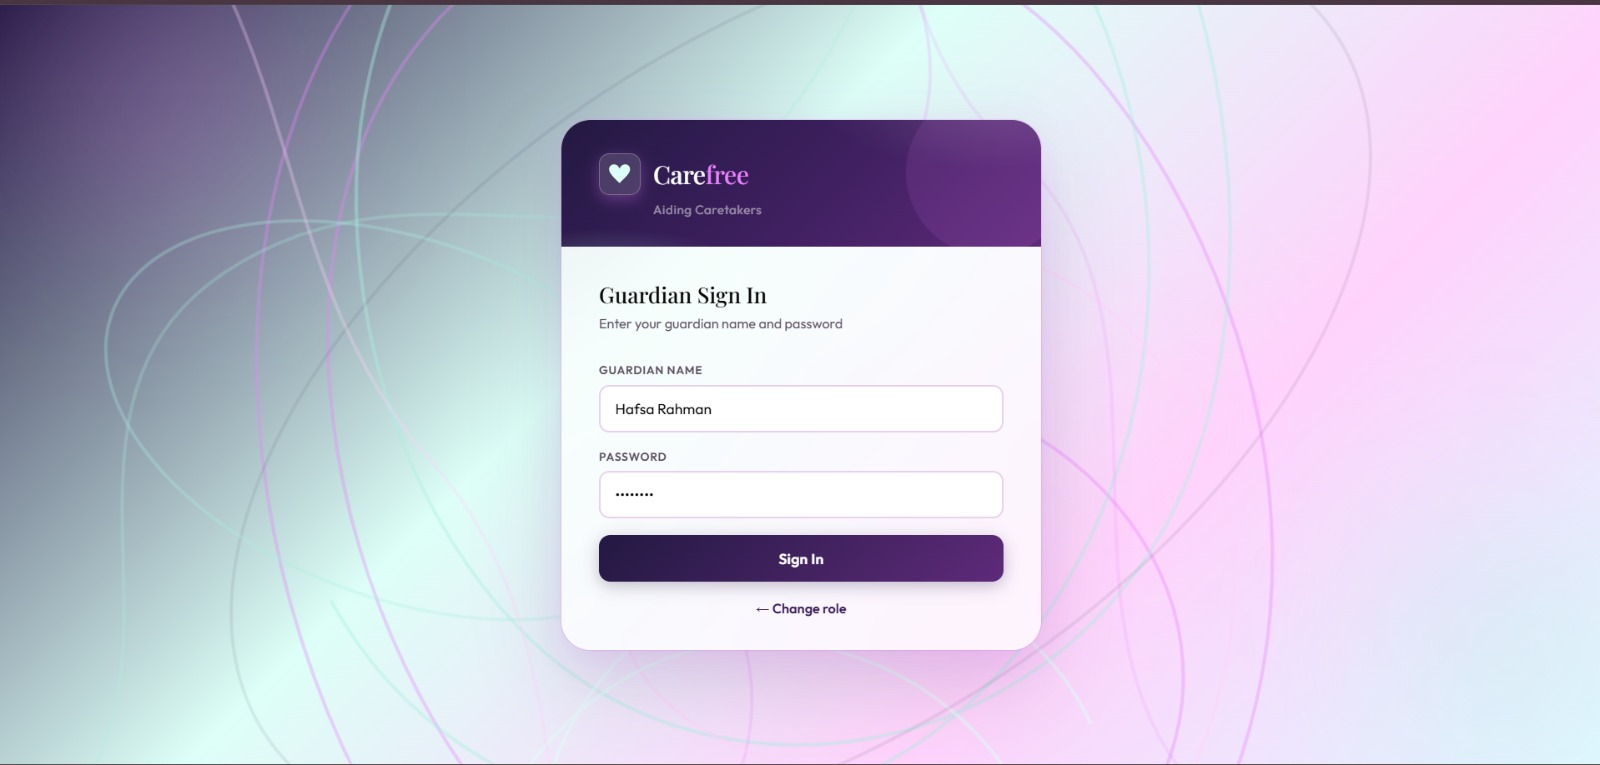
\includegraphics[width=0.85\textwidth]{external_schema/guardian_signin.jpeg}
    \caption{Guardian Sign In}
\end{figure}

\subsubsection{Caretaker Views}
\begin{figure}[H]
    \centering
    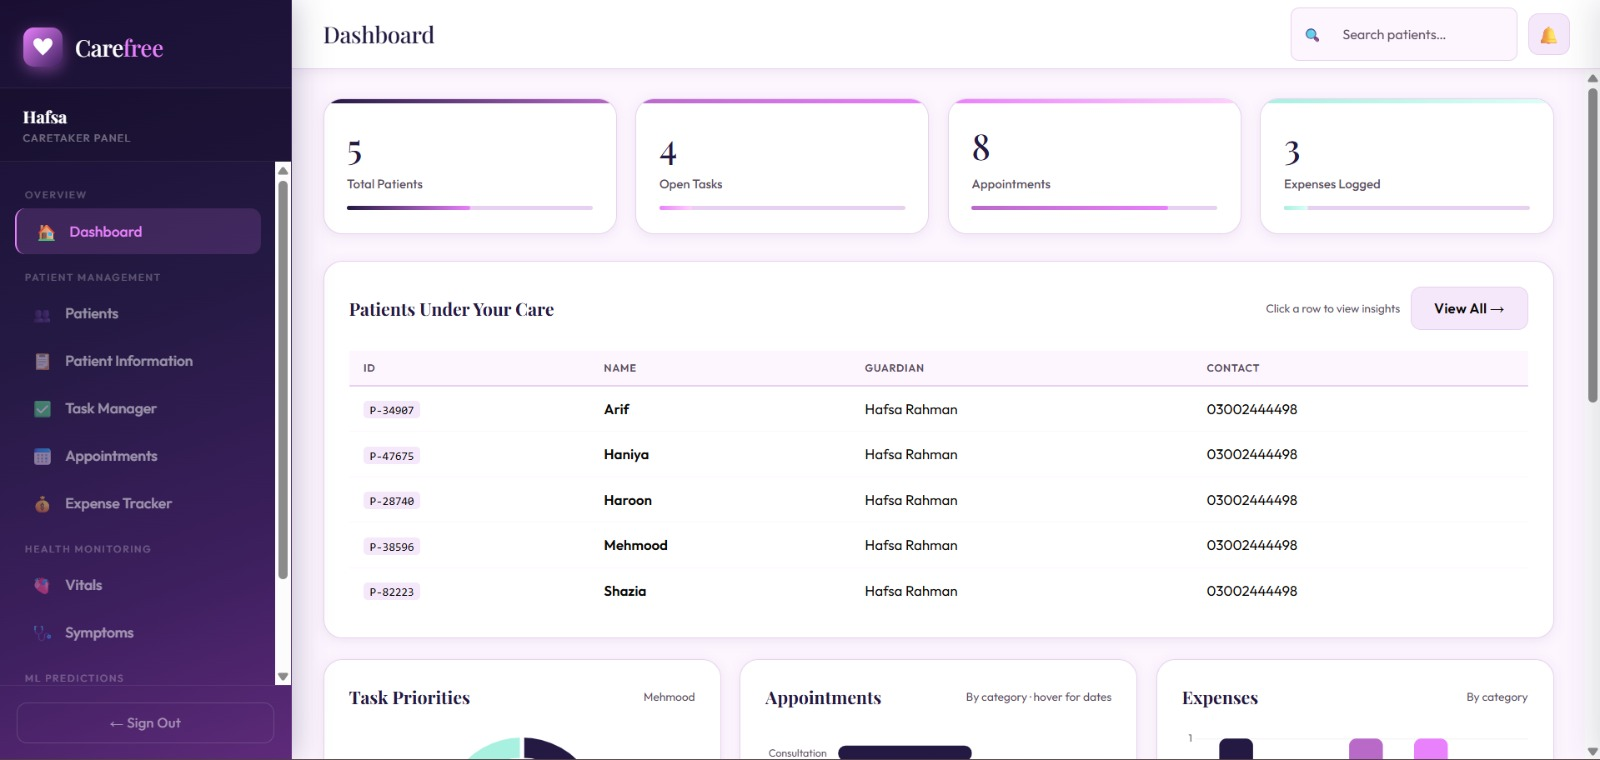
\includegraphics[width=0.85\textwidth]{external_schema/caretaker_dash1.jpeg}
    \caption{Caretaker Dashboard}
\end{figure}
\begin{figure}[H]
    \centering
    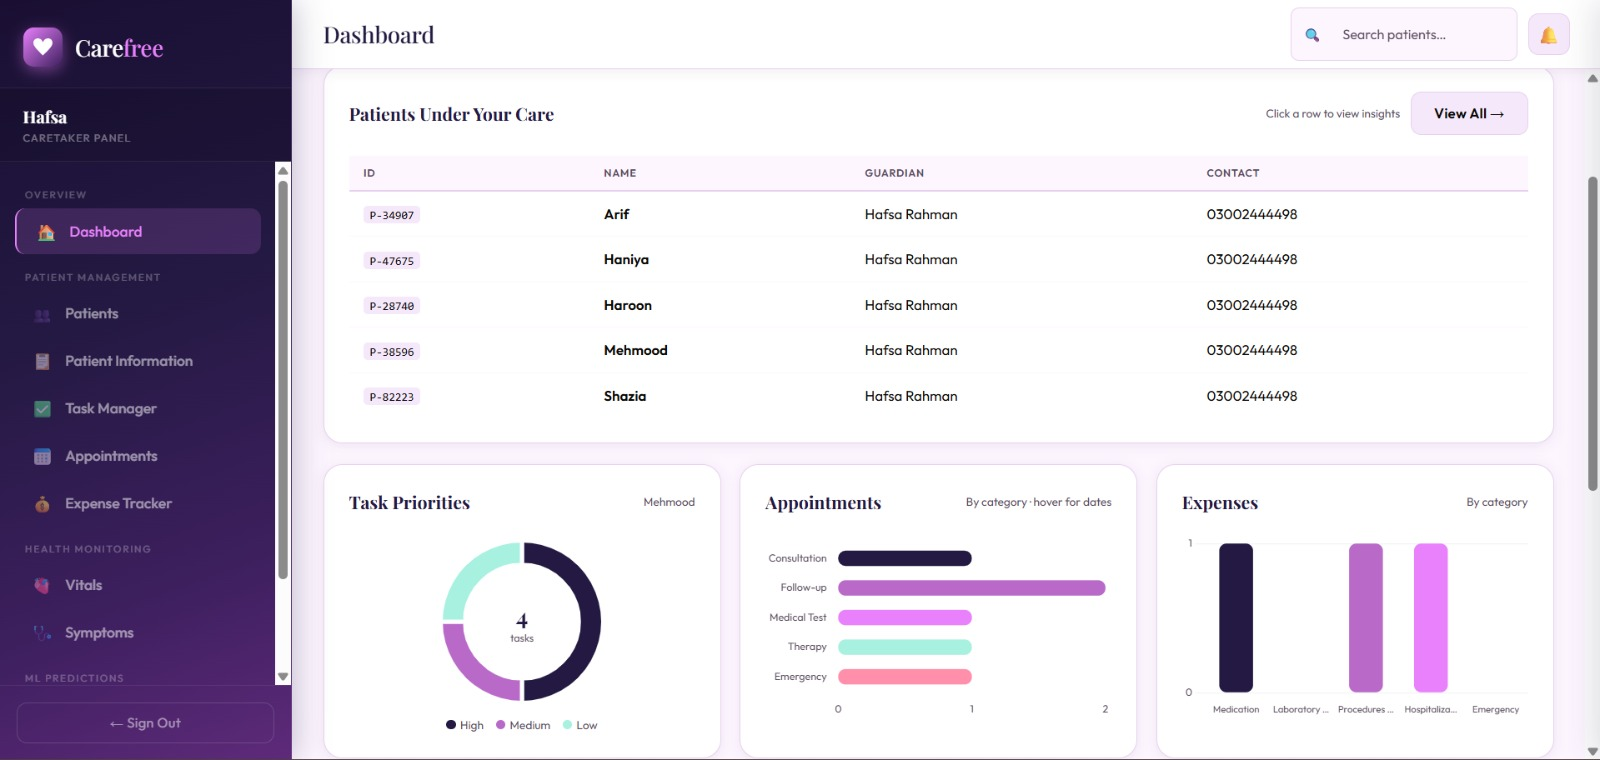
\includegraphics[width=0.85\textwidth]{external_schema/caretaker_dash2.jpeg}
    \caption{Caretaker Dashboard: Continued}
\end{figure}
\begin{figure}[H]
    \centering
    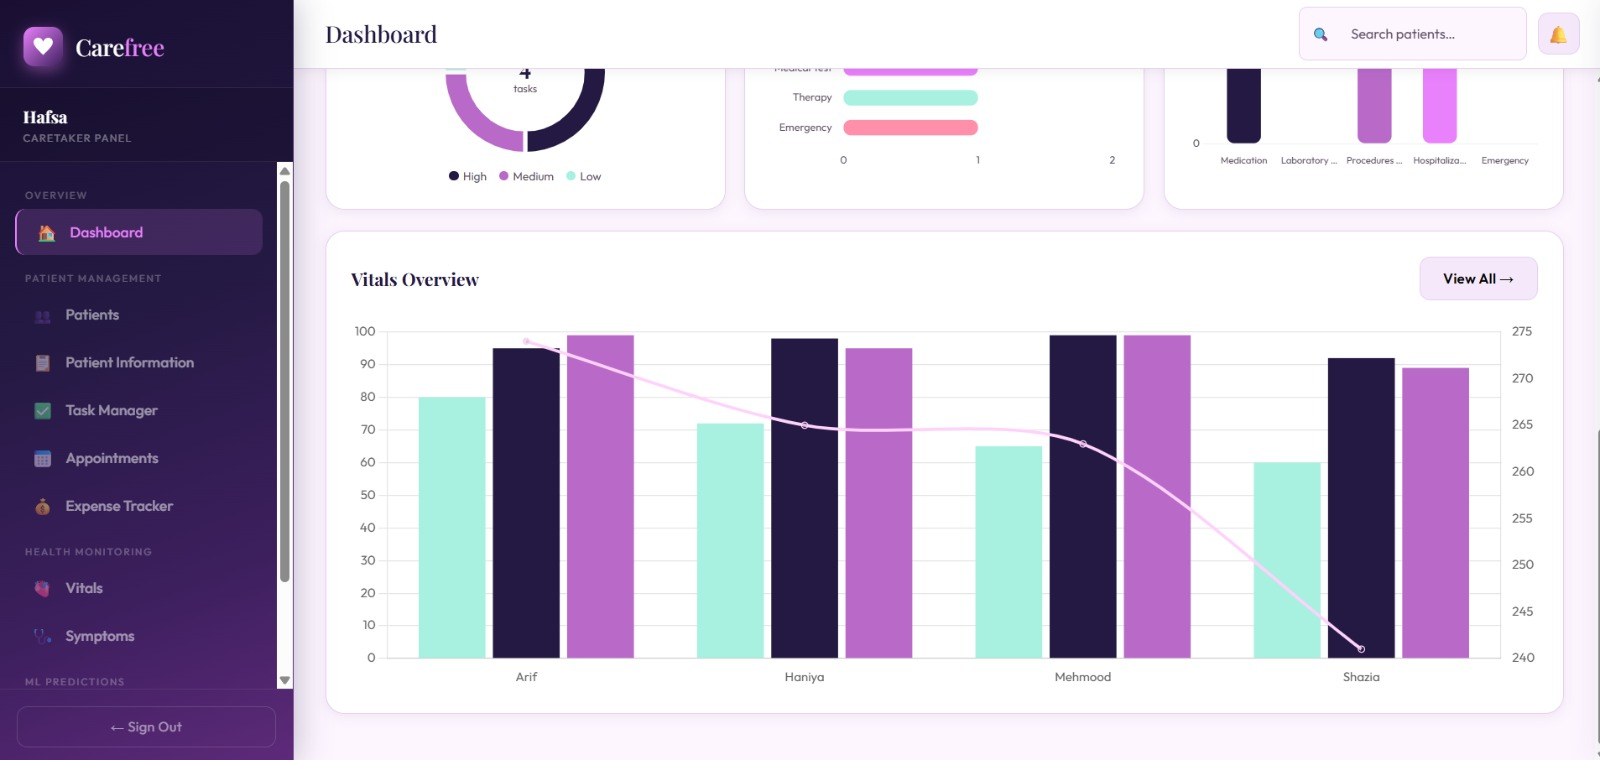
\includegraphics[width=0.85\textwidth]{external_schema/caretaker_dash3.jpeg}
    \caption{Caretaker Dashboard: Continued}
\end{figure}
\begin{figure}[H]
    \centering
    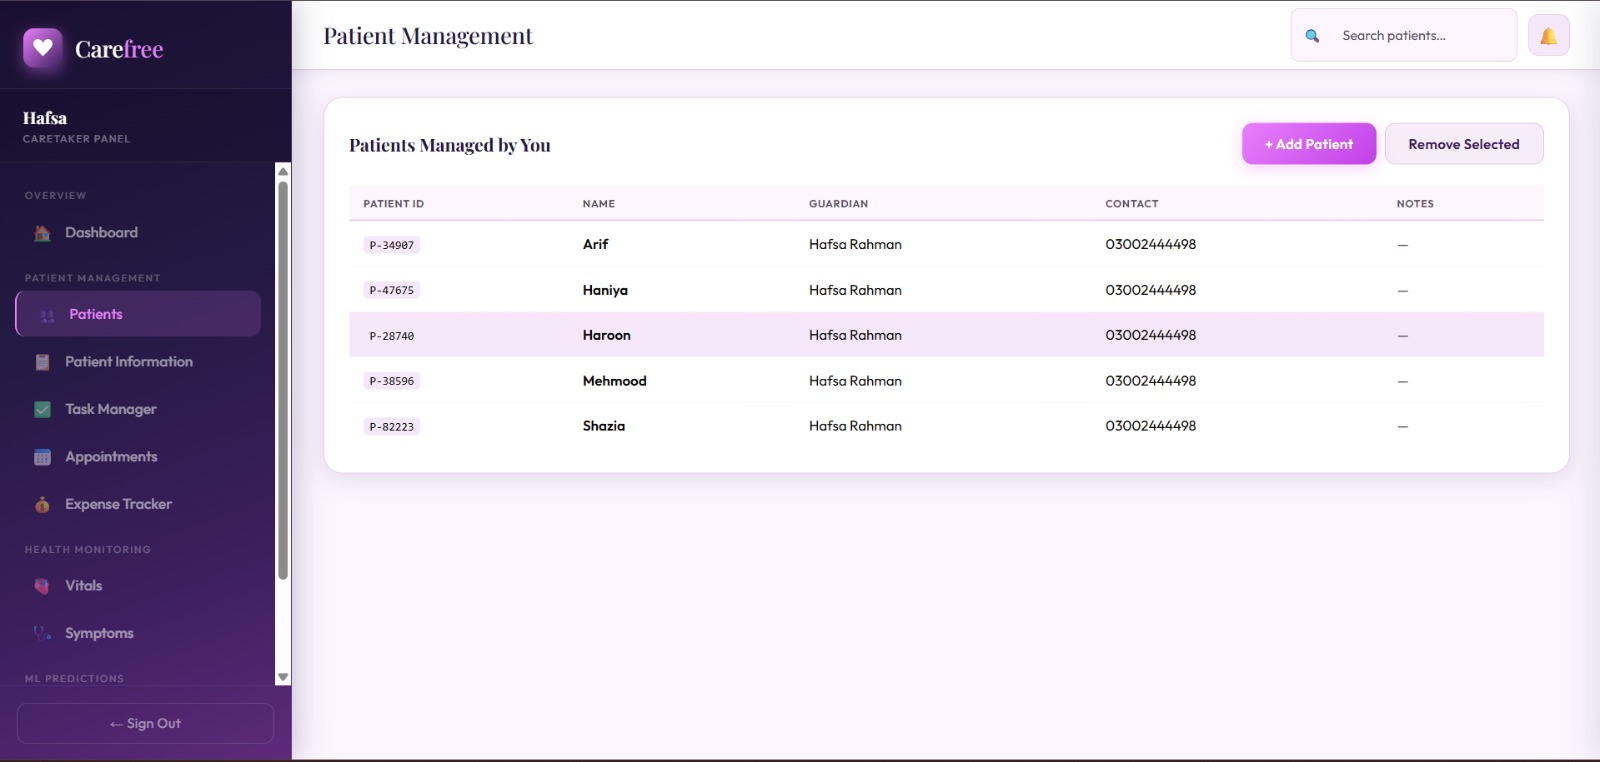
\includegraphics[width=0.85\textwidth]{external_schema/caretaker_dash4.jpeg}
    \caption{Caretaker Dashboard: Continued}
\end{figure}
\begin{figure}[H]
    \centering
    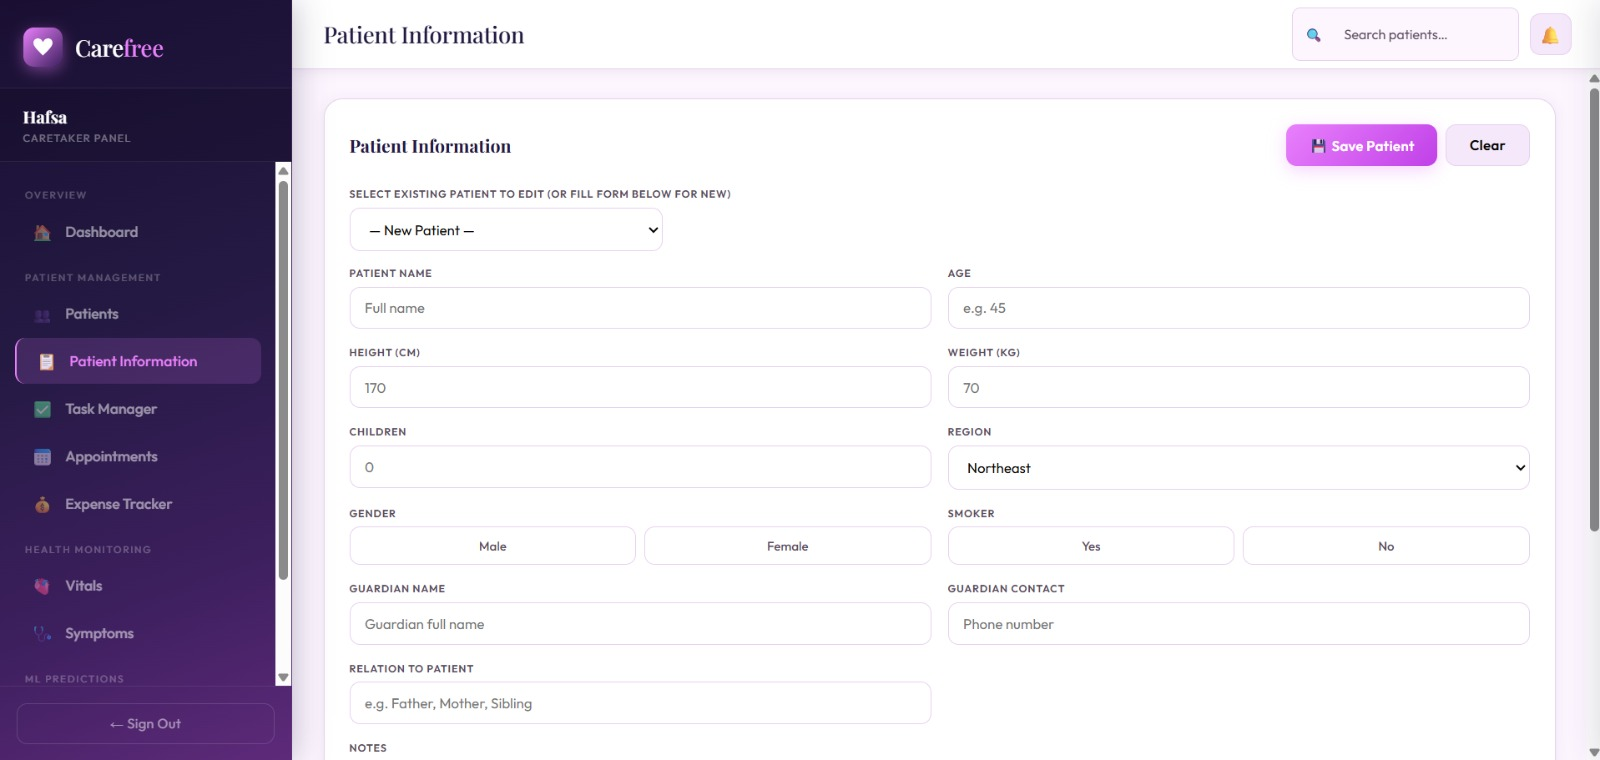
\includegraphics[width=0.85\textwidth]{external_schema/patient_info1.jpeg}
    \caption{Patient Information }
\end{figure}
\begin{figure}[H]
    \centering
    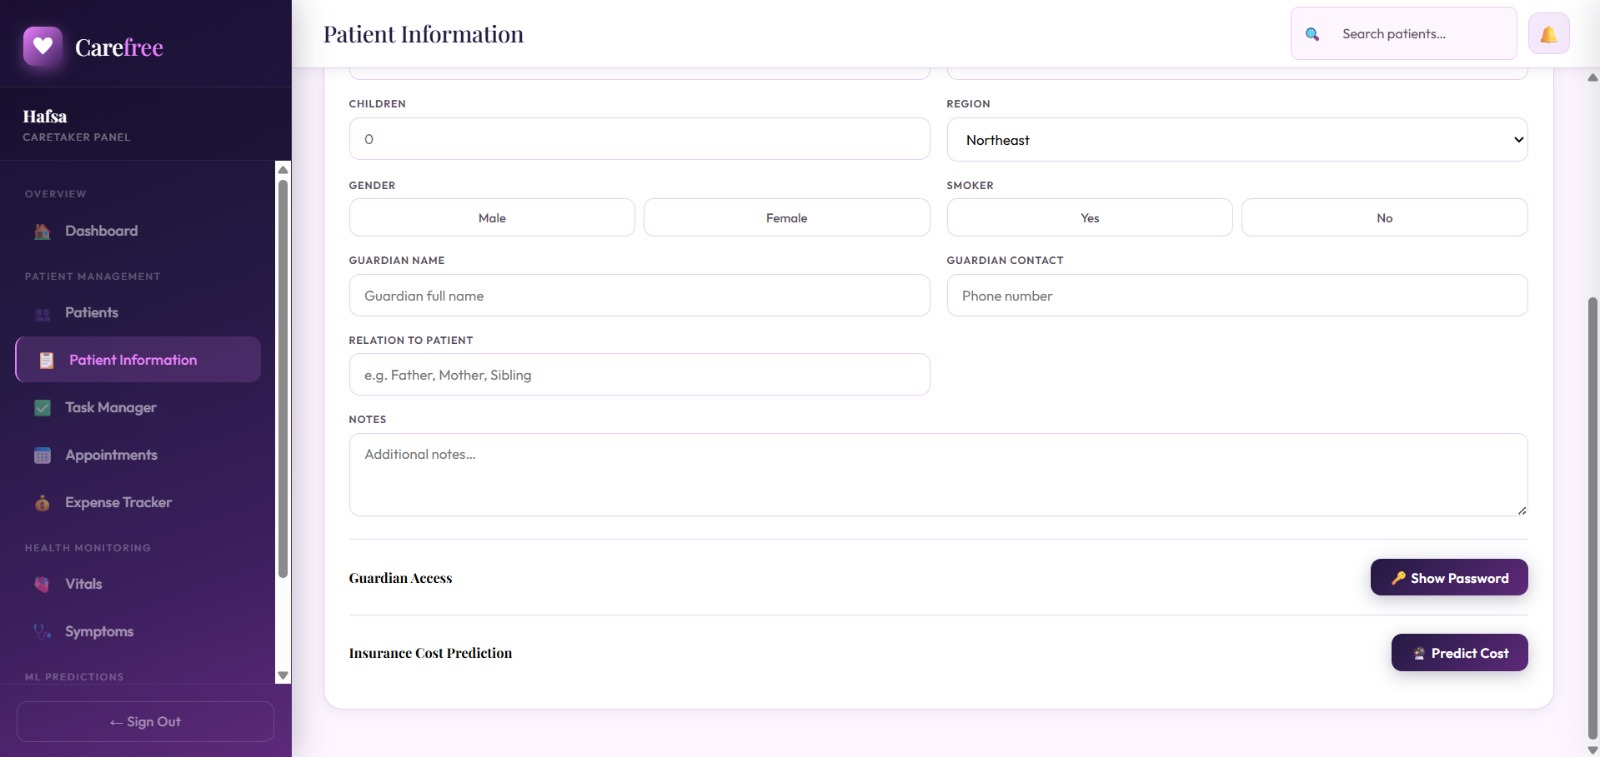
\includegraphics[width=0.85\textwidth]{external_schema/patient_info2.jpeg}
    \caption{Patient Information: Continued}
\end{figure}
\begin{figure}[H]
    \centering
    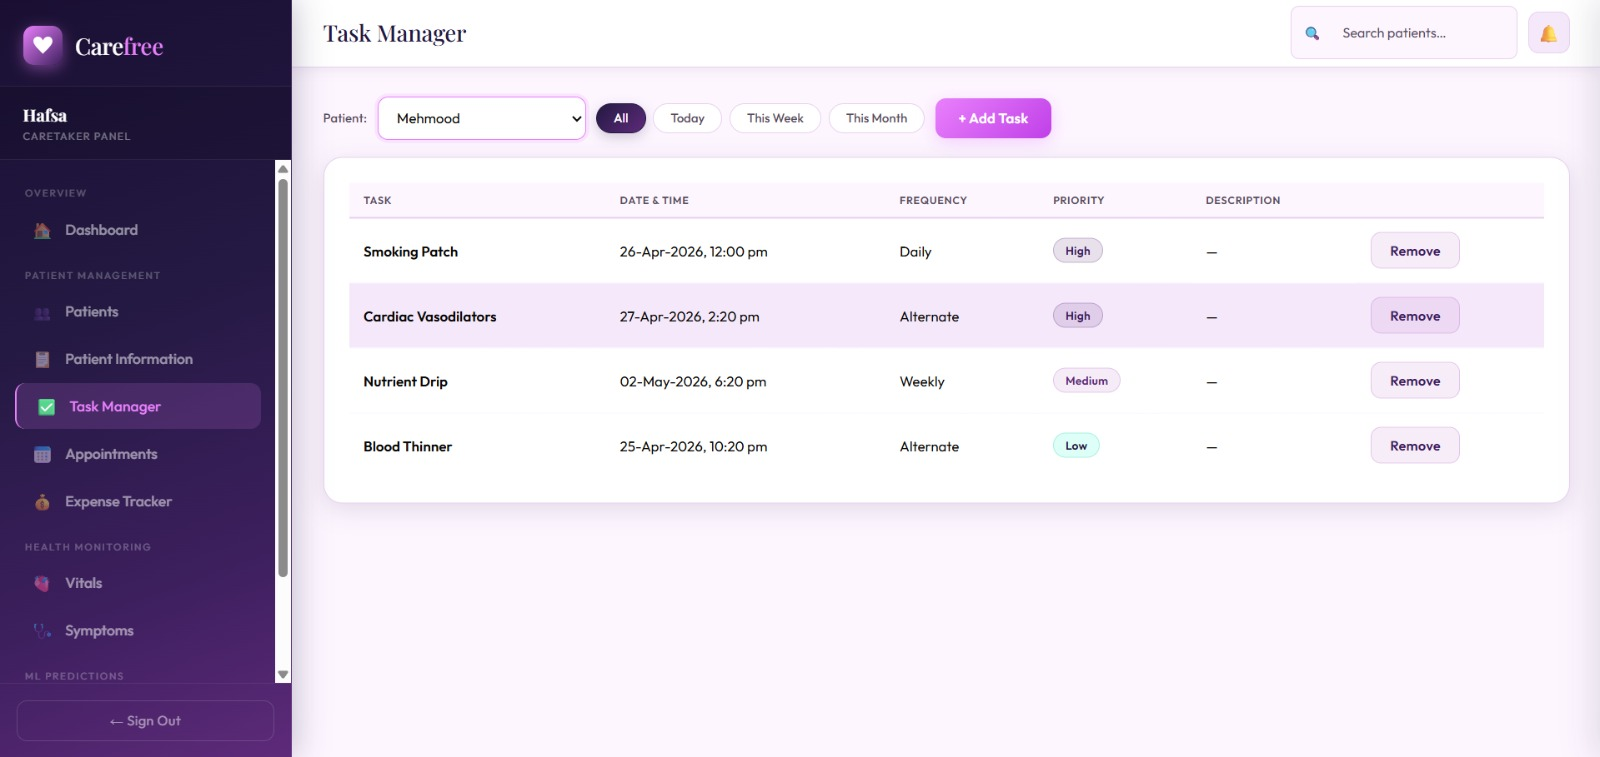
\includegraphics[width=0.85\textwidth]{external_schema/task_manager1.jpeg}
    \caption{Task Manager}
\end{figure}
\begin{figure}[H]
    \centering
    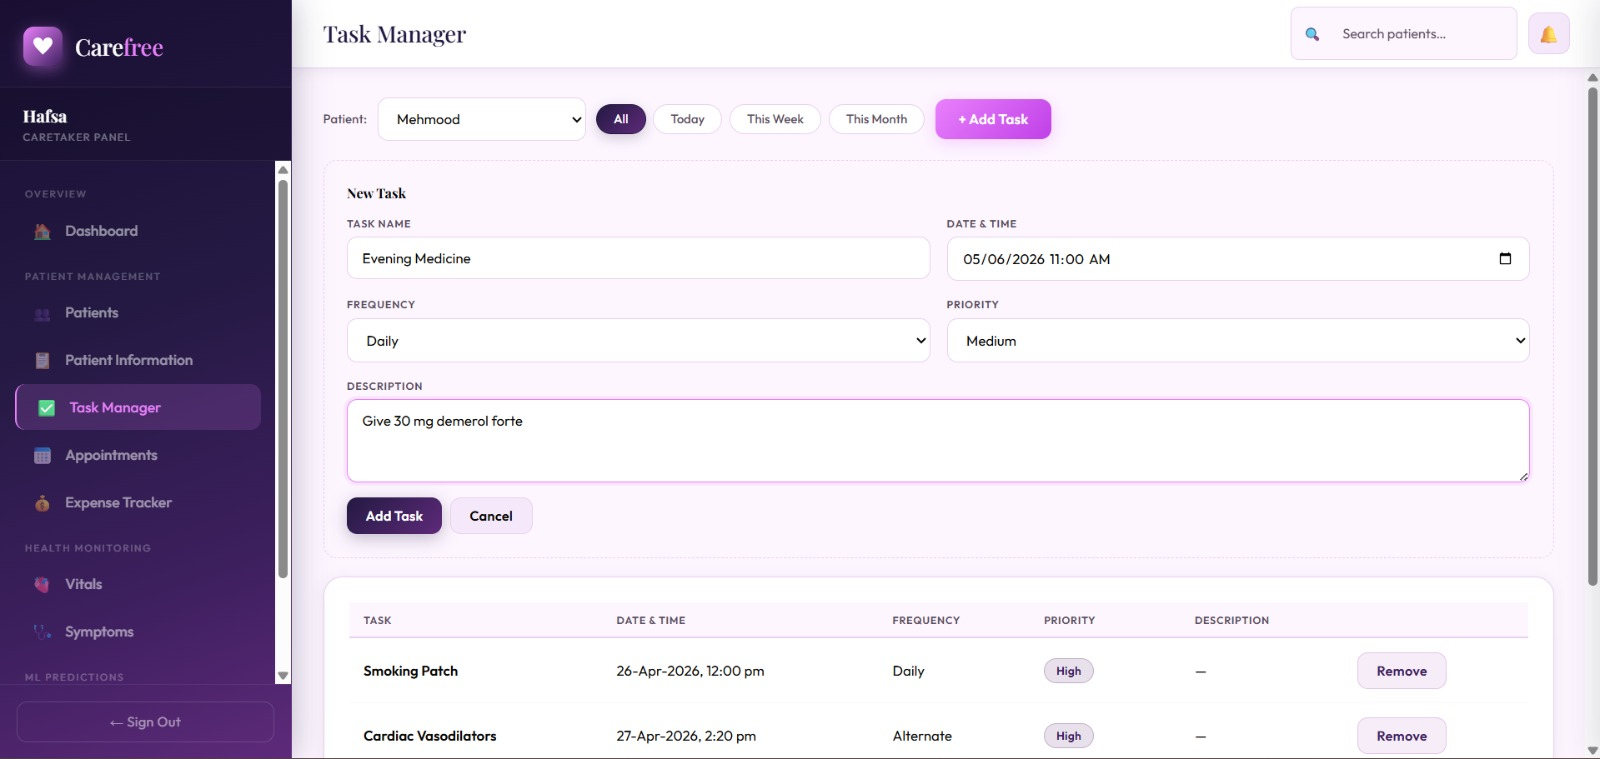
\includegraphics[width=0.85\textwidth]{external_schema/task_manager2.jpeg}
    \caption{Task Manager: Continued}
\end{figure}
\begin{figure}[H]
    \centering
    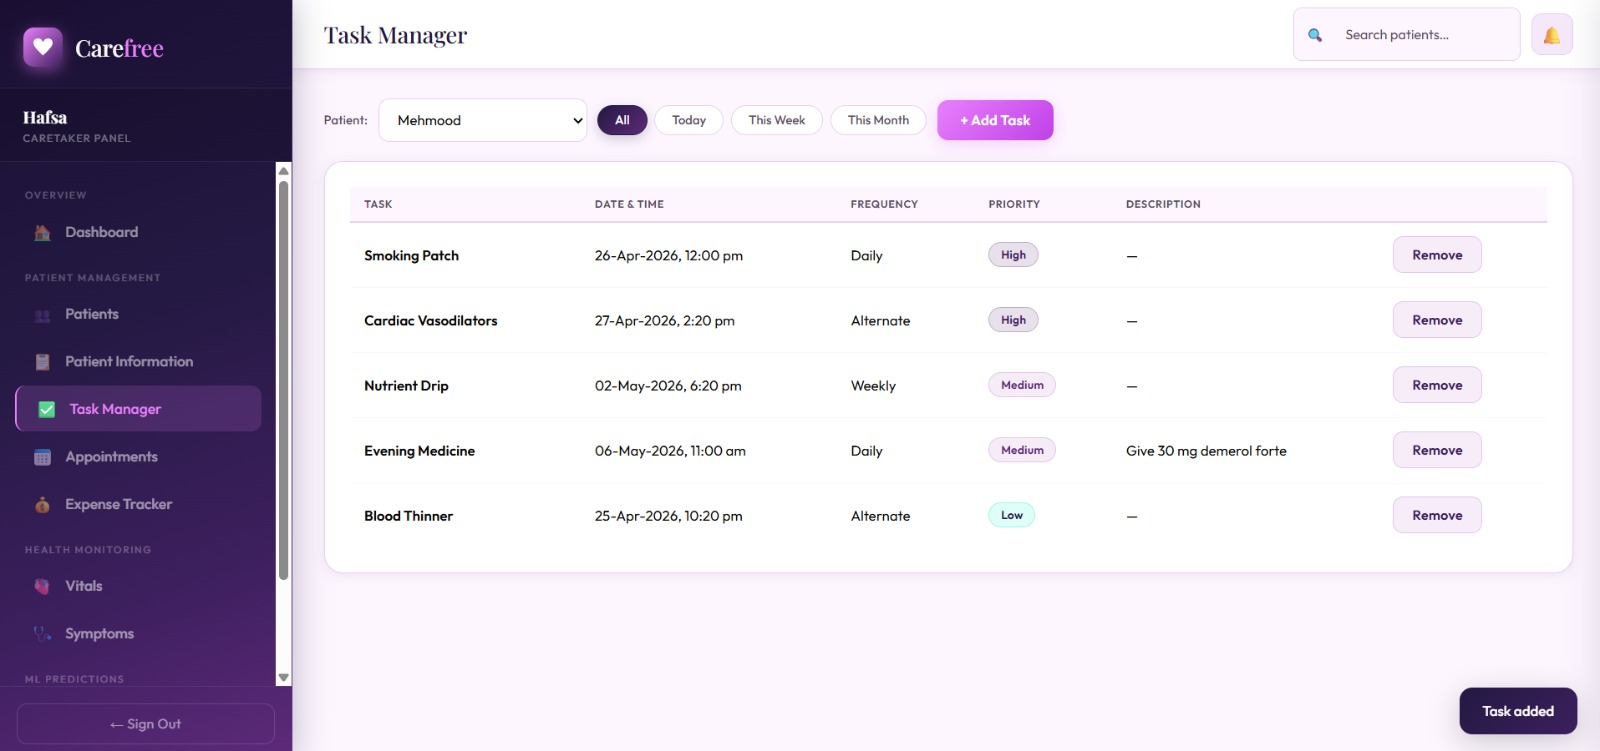
\includegraphics[width=0.85\textwidth]{external_schema/task_manager3.jpeg}
    \caption{Task Manager: Continued}
\end{figure}
\begin{figure}[H]
    \centering
    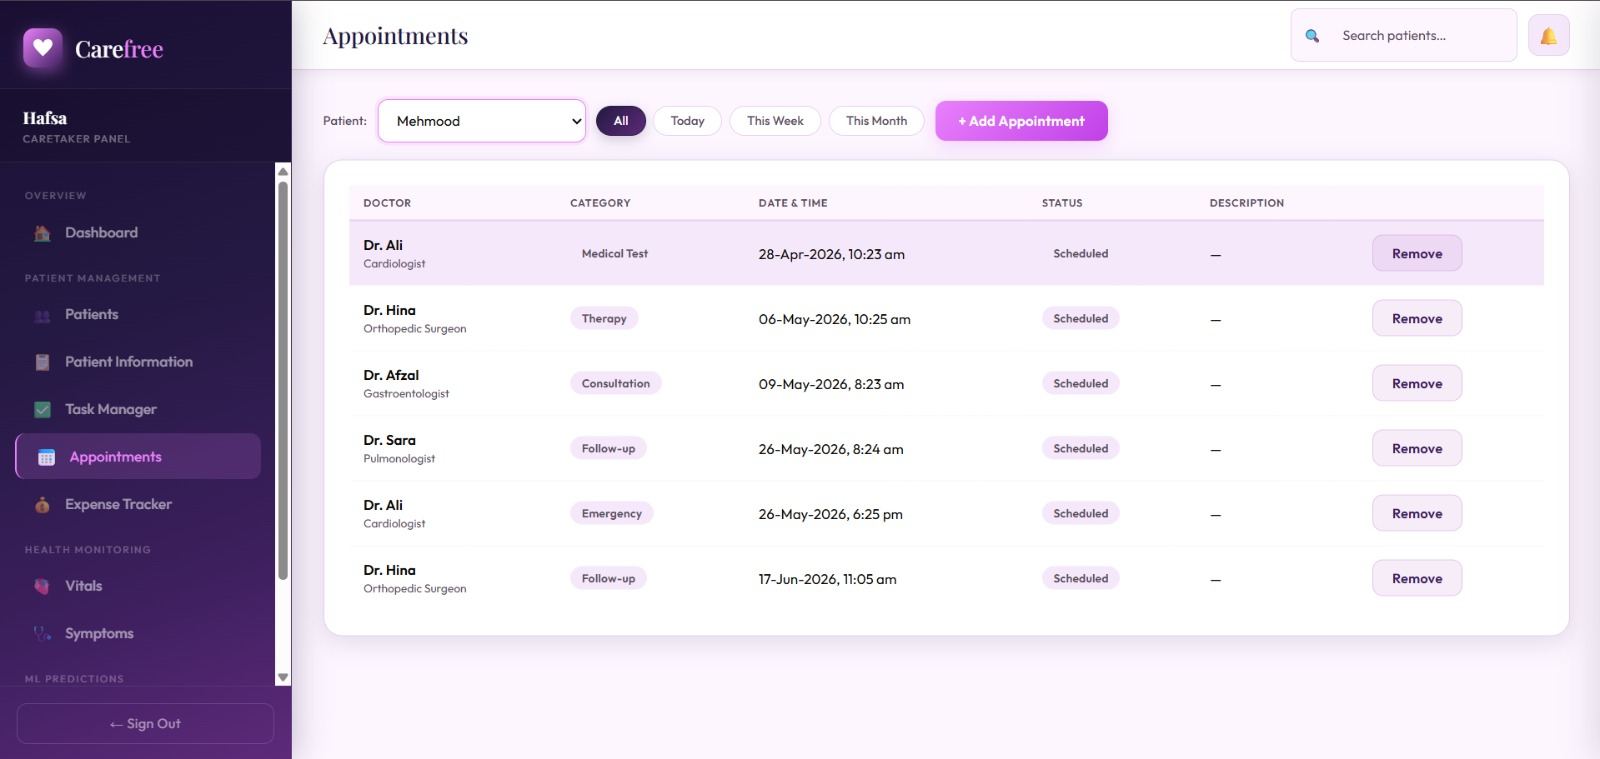
\includegraphics[width=0.85\textwidth]{external_schema/appointments1.jpeg}
    \caption{Appointments}
\end{figure}
\begin{figure}[H]
    \centering
    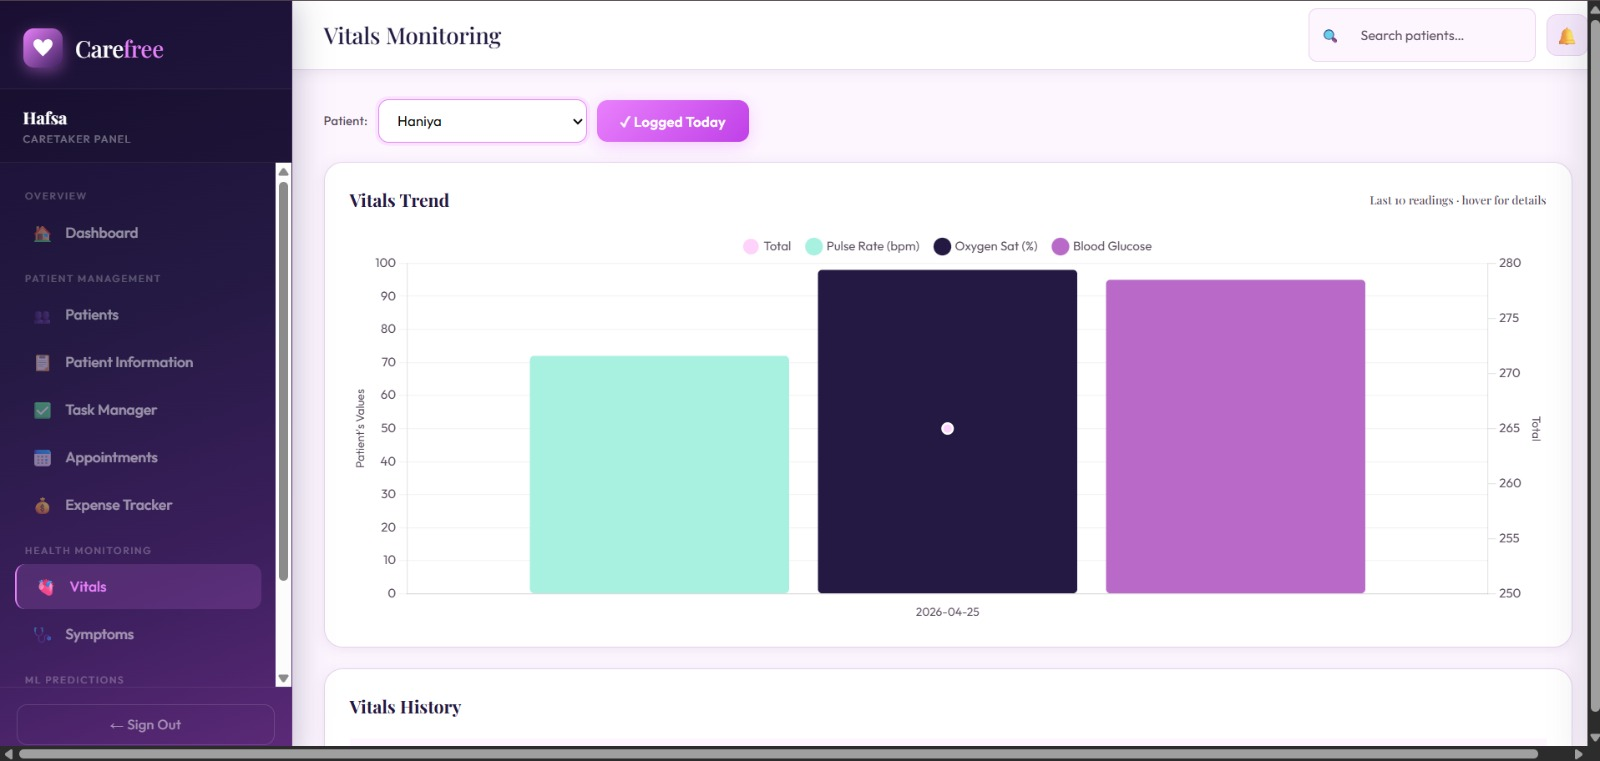
\includegraphics[width=0.85\textwidth]{external_schema/vitals1.jpeg}
    \caption{Vitals Tracker}
\end{figure}
\begin{figure}[H]
    \centering
    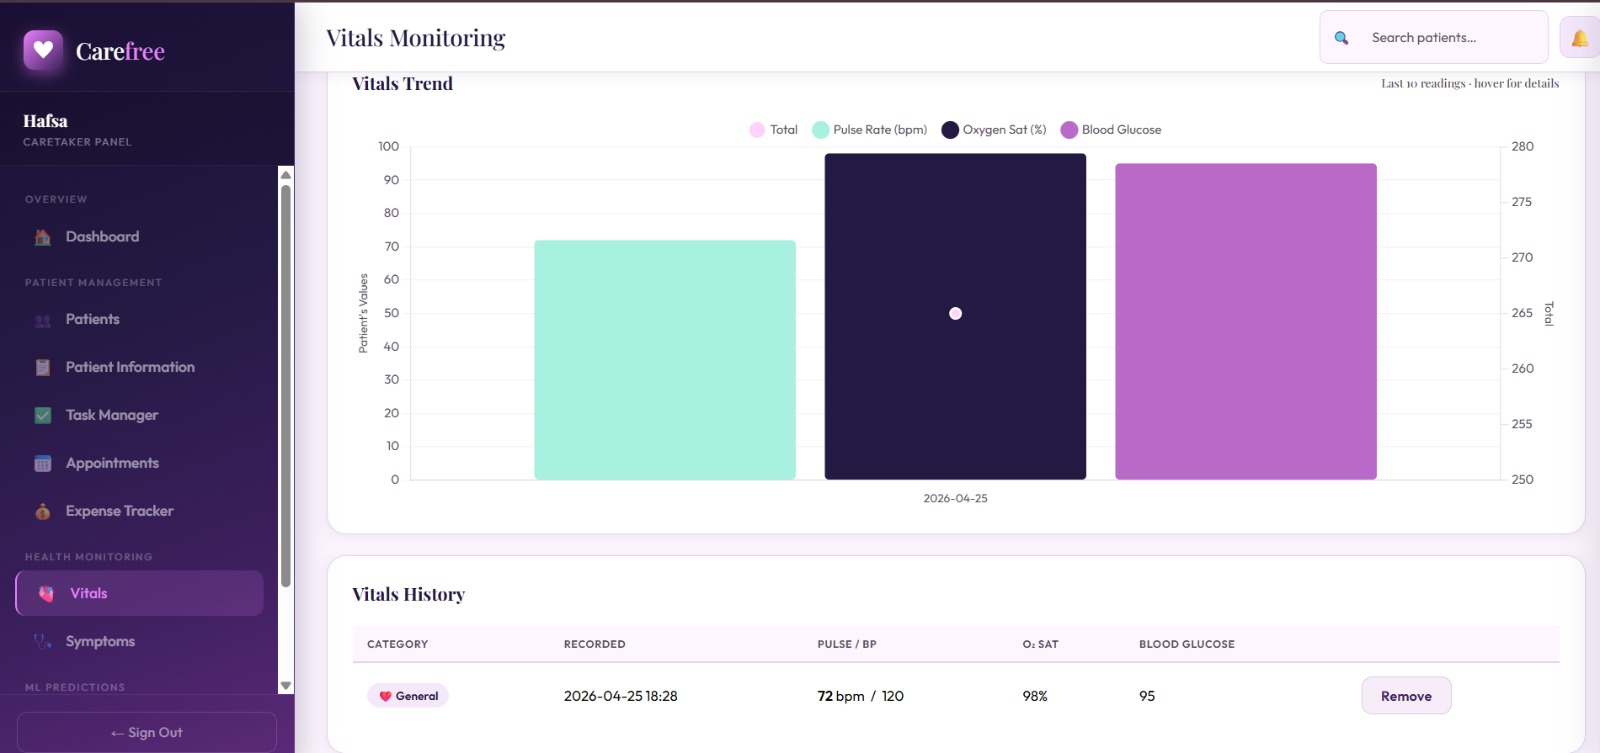
\includegraphics[width=0.85\textwidth]{external_schema/vitals2.jpeg}
    \caption{Vitals Tracker: Continued}
\end{figure}
\begin{figure}[H]
    \centering
    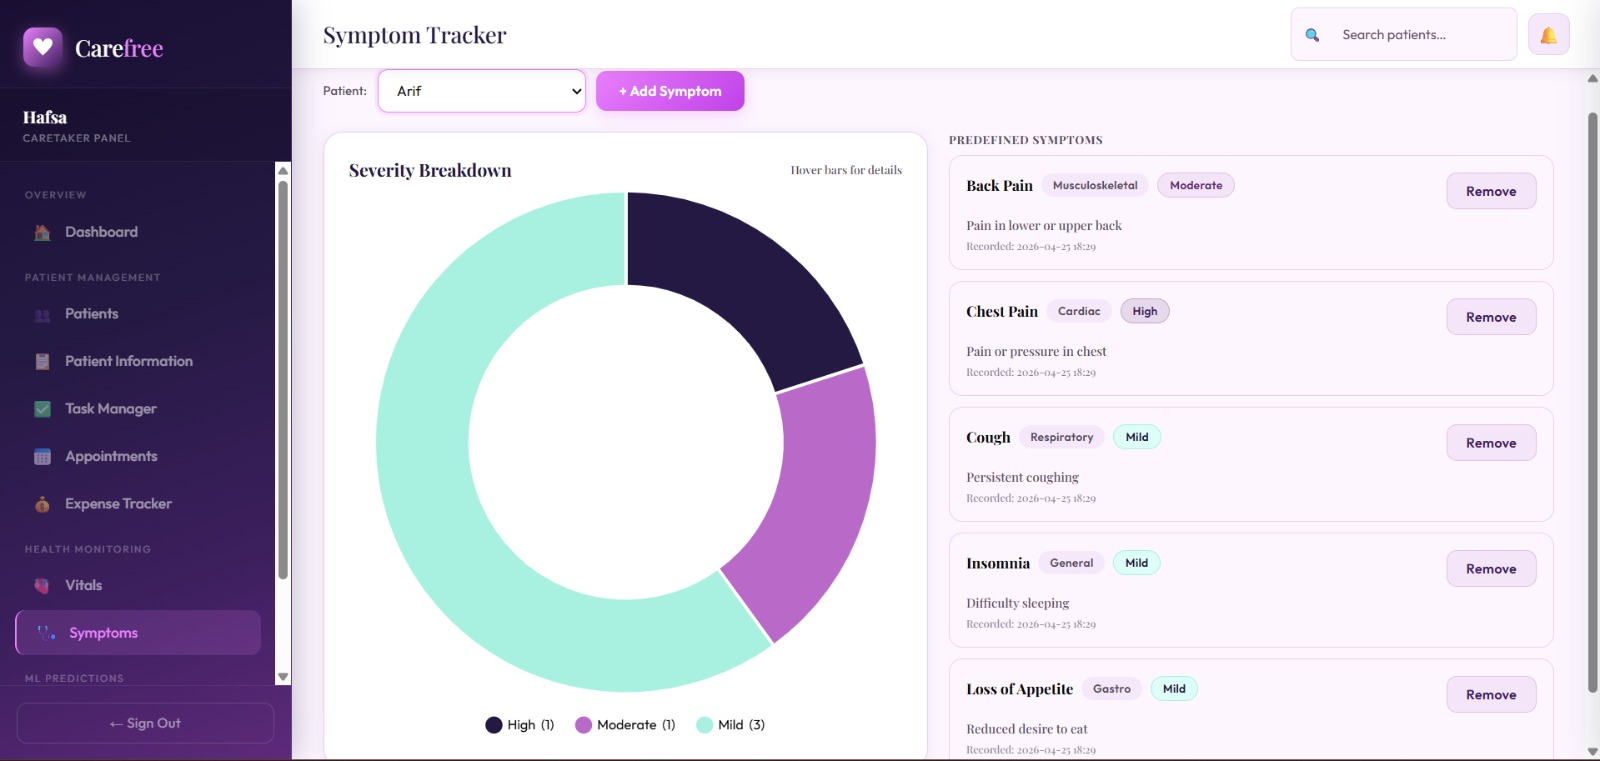
\includegraphics[width=0.85\textwidth]{external_schema/symptoms1.jpeg}
    \caption{Symptom Logger}
\end{figure}
\begin{figure}[H]
    \centering
    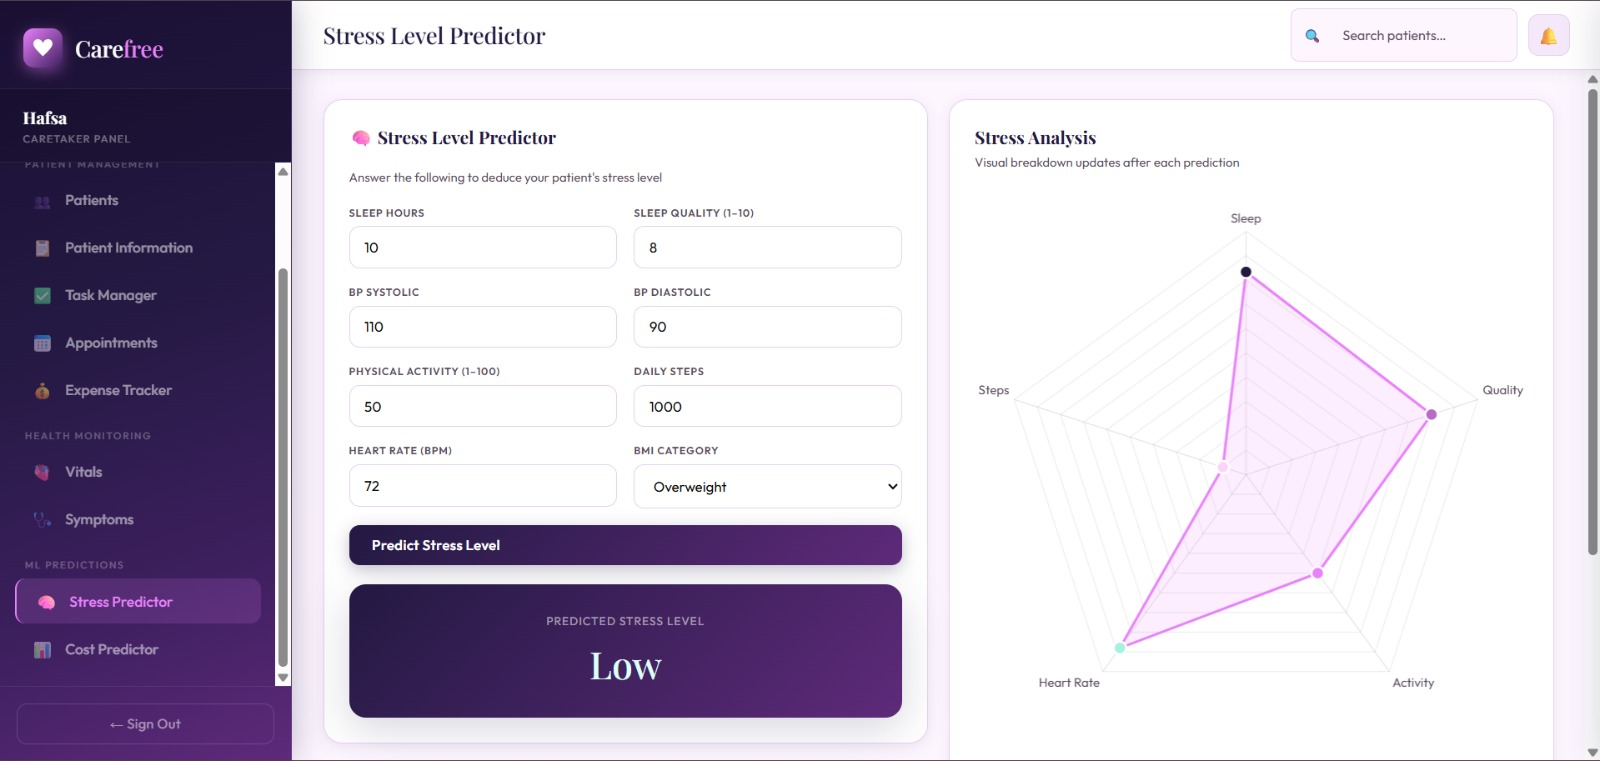
\includegraphics[width=0.85\textwidth]{external_schema/stress_predictor1.jpeg}
    \caption{ML Stress Predictor}
\end{figure}
\begin{figure}[H]
    \centering
    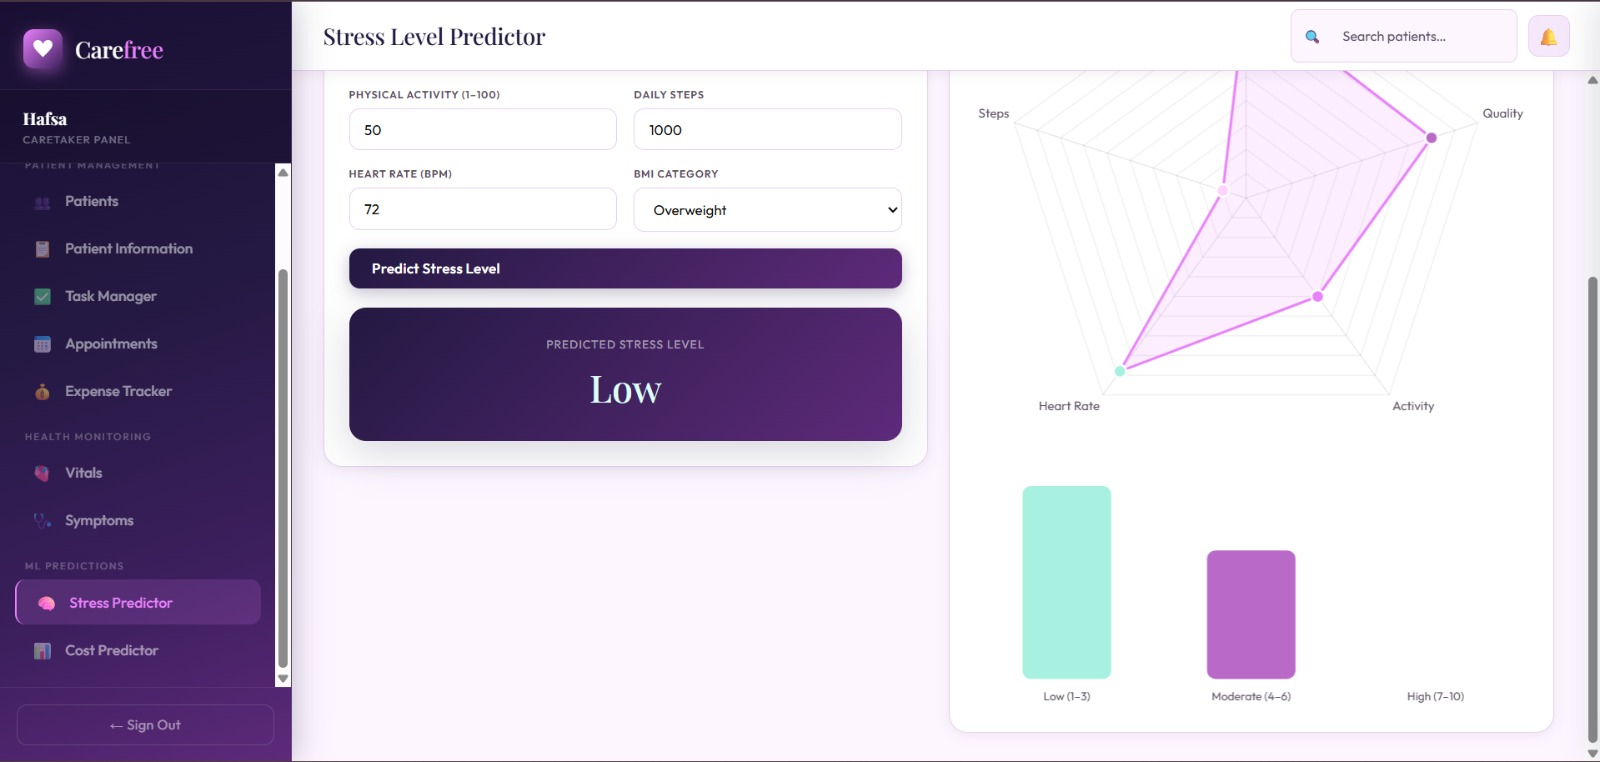
\includegraphics[width=0.85\textwidth]{external_schema/stress_predictor2.jpeg}
    \caption{ML Stress Predictor: Continued}
\end{figure}
\begin{figure}[H]
    \centering
    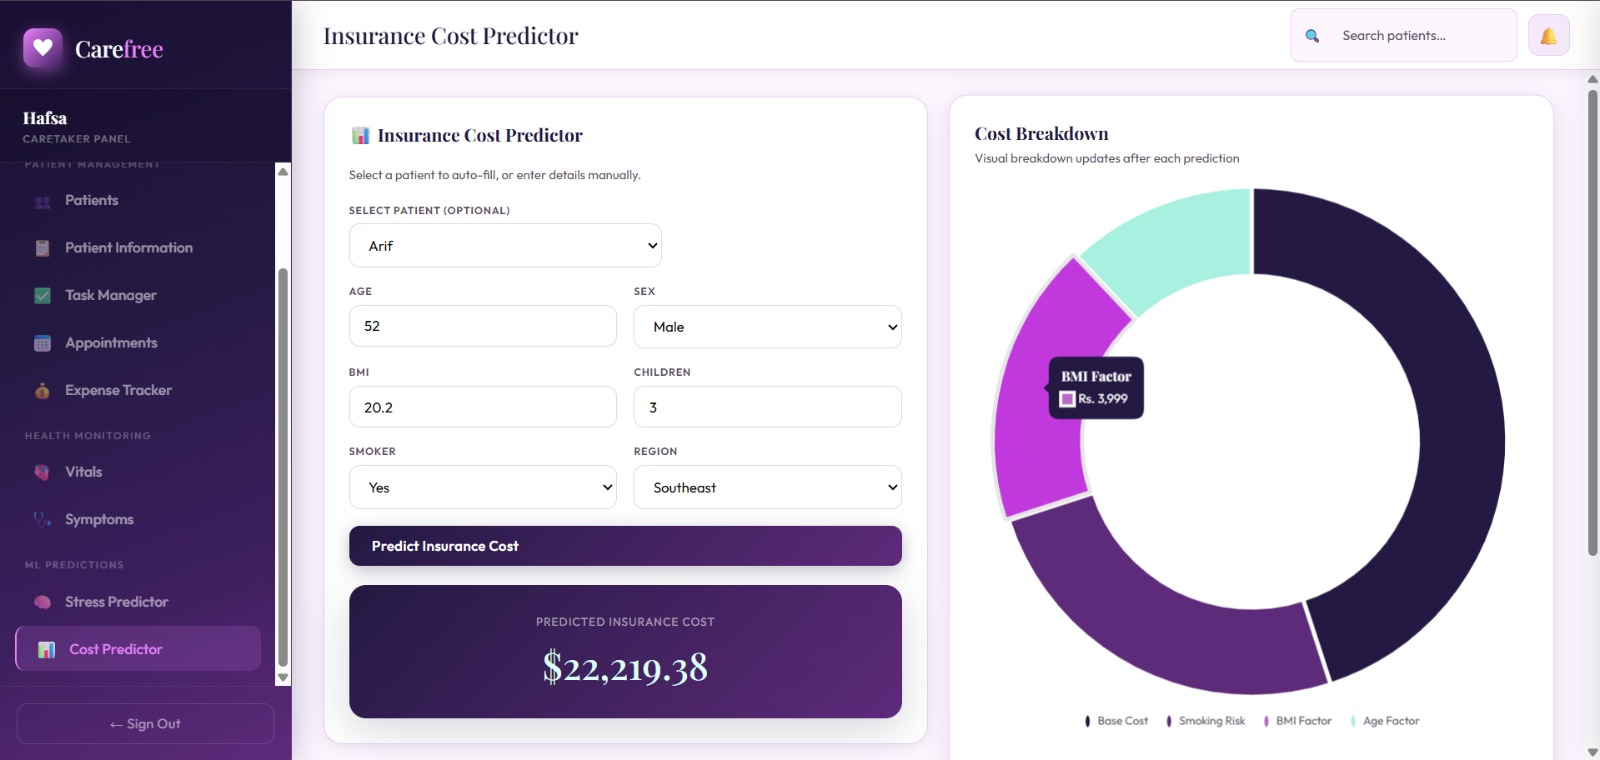
\includegraphics[width=0.85\textwidth]{external_schema/medical_cost1.jpeg}
    \caption{ML medical cost predictor}
\end{figure}
\begin{figure}[H]
    \centering
    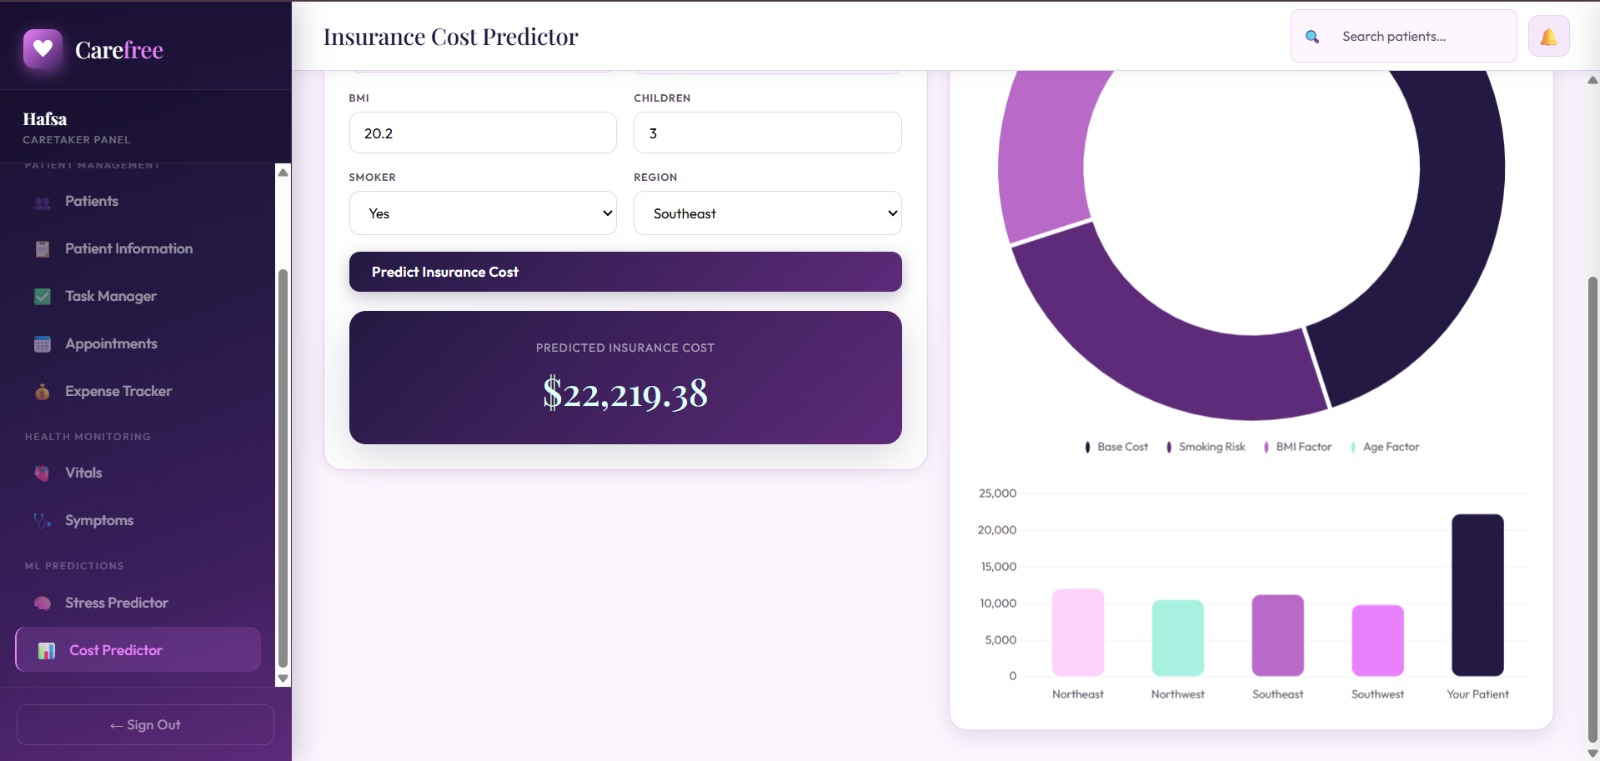
\includegraphics[width=0.85\textwidth]{external_schema/medical_cost2.jpeg}
    \caption{ML medical cost predictor: Continued}
\end{figure}

\subsubsection{Guardian Views}
\begin{figure}[H]
    \centering
    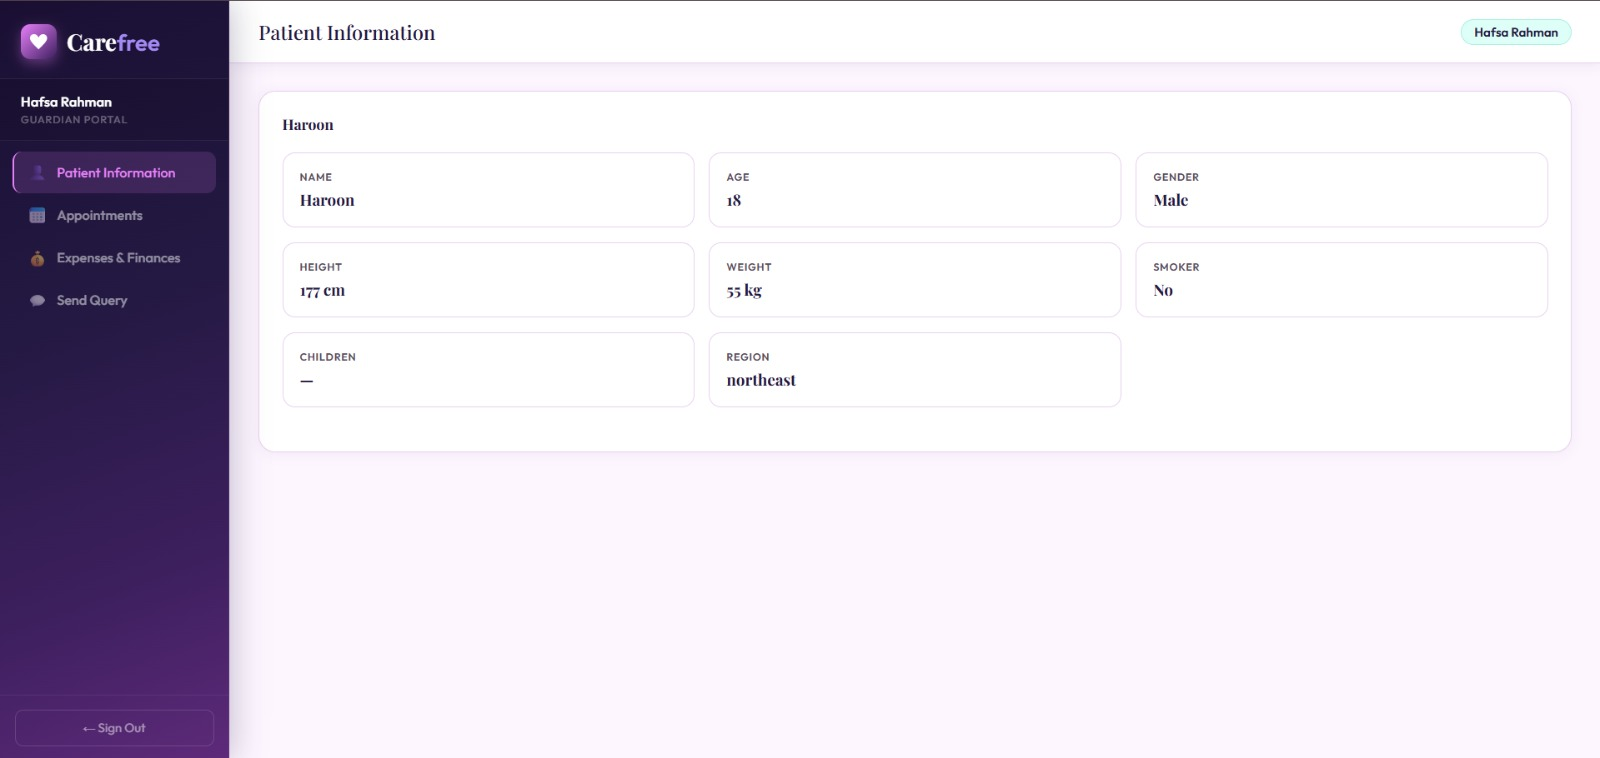
\includegraphics[width=0.85\textwidth]{external_schema/guardian_patient_info.jpeg}
    \caption{Patient Information}
\end{figure}
\begin{figure}[H]
    \centering
    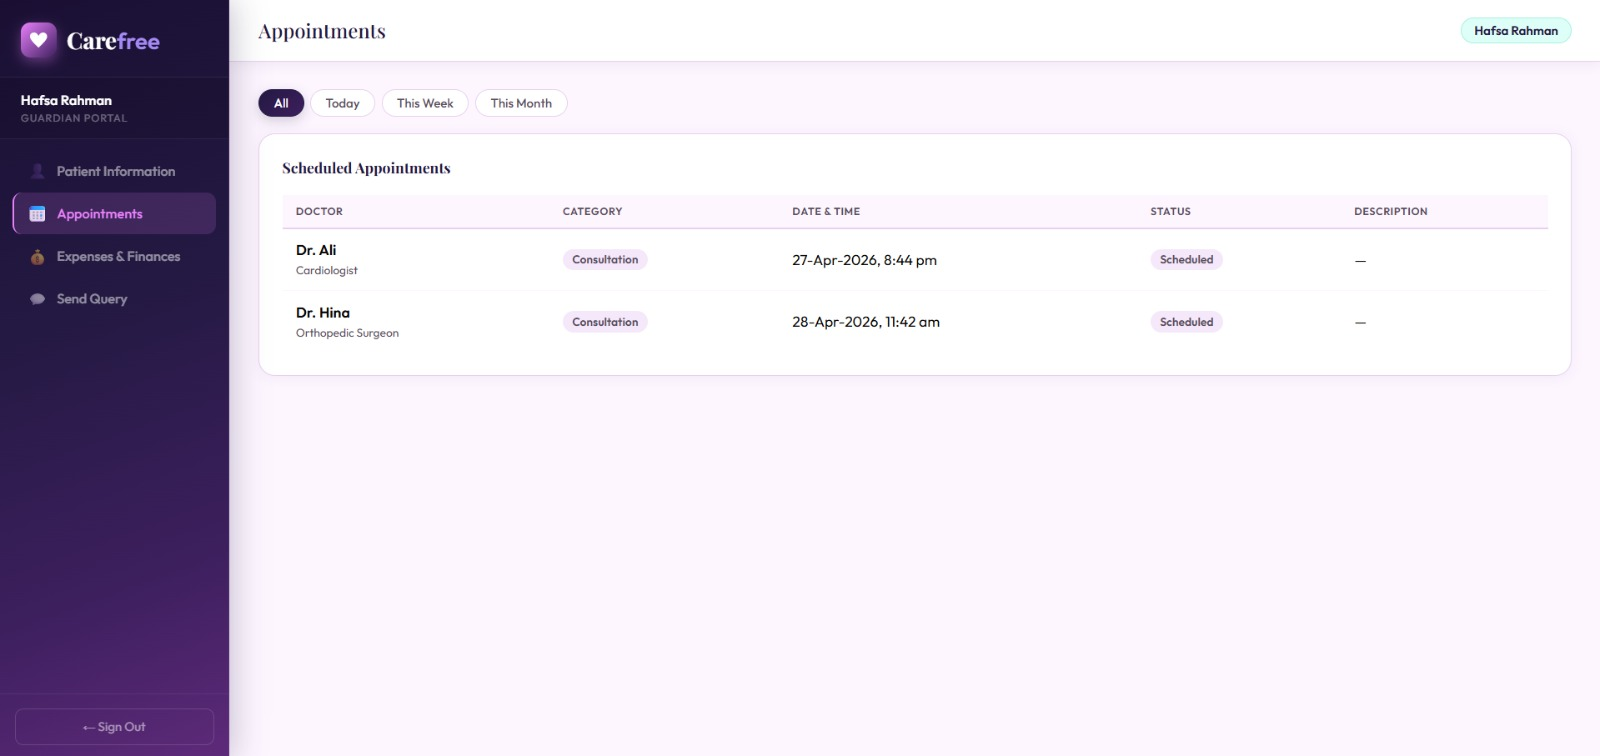
\includegraphics[width=0.85\textwidth]{external_schema/guardian_appointment.jpeg}
    \caption{Appointment}
\end{figure}
\begin{figure}[H]
    \centering
    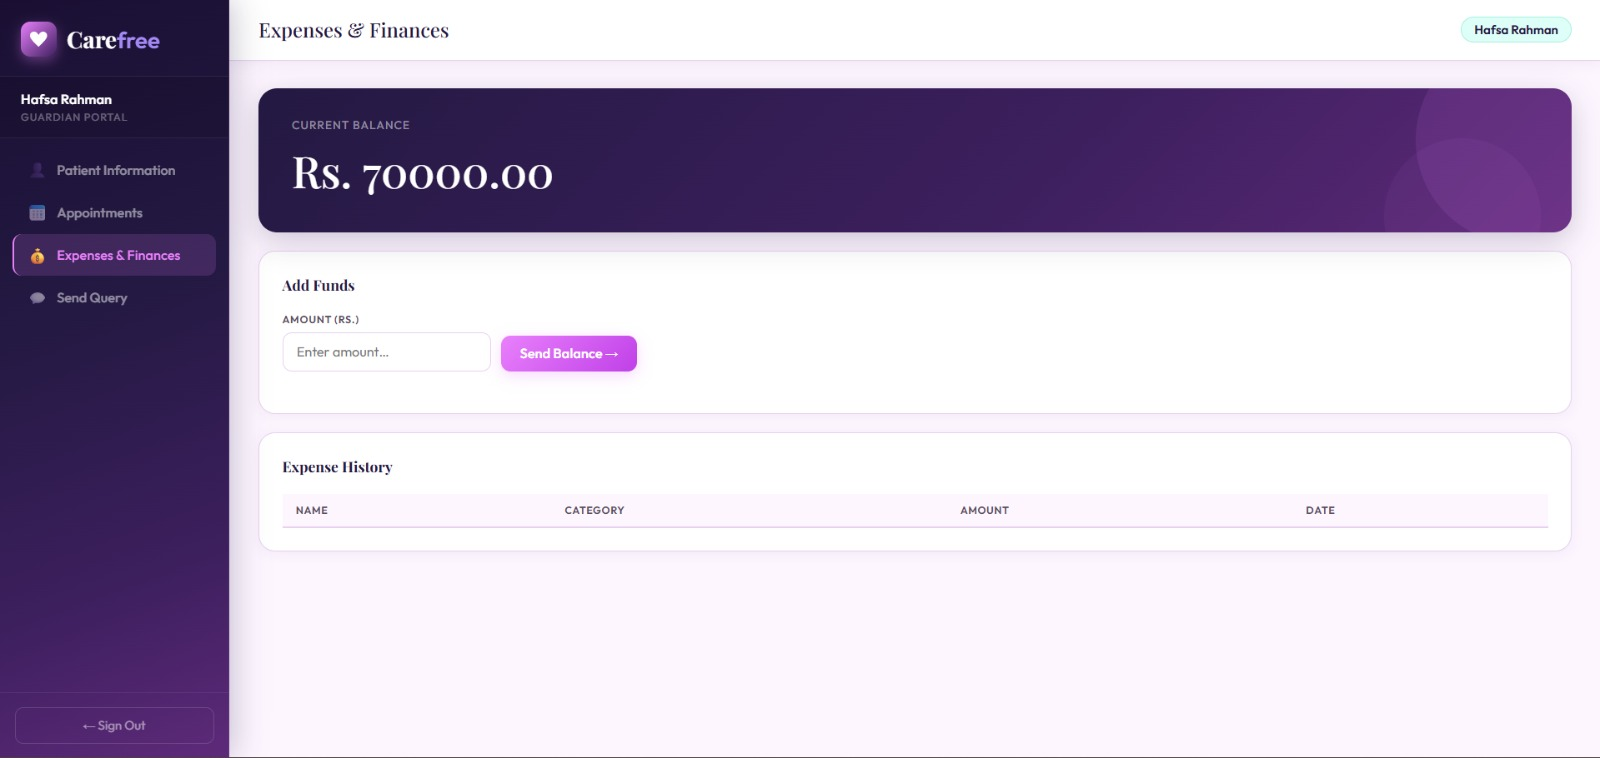
\includegraphics[width=0.85\textwidth]{external_schema/guardian_expense.jpeg}
    \caption{Expense Tracker}
\end{figure}
\begin{figure}[H]
    \centering
    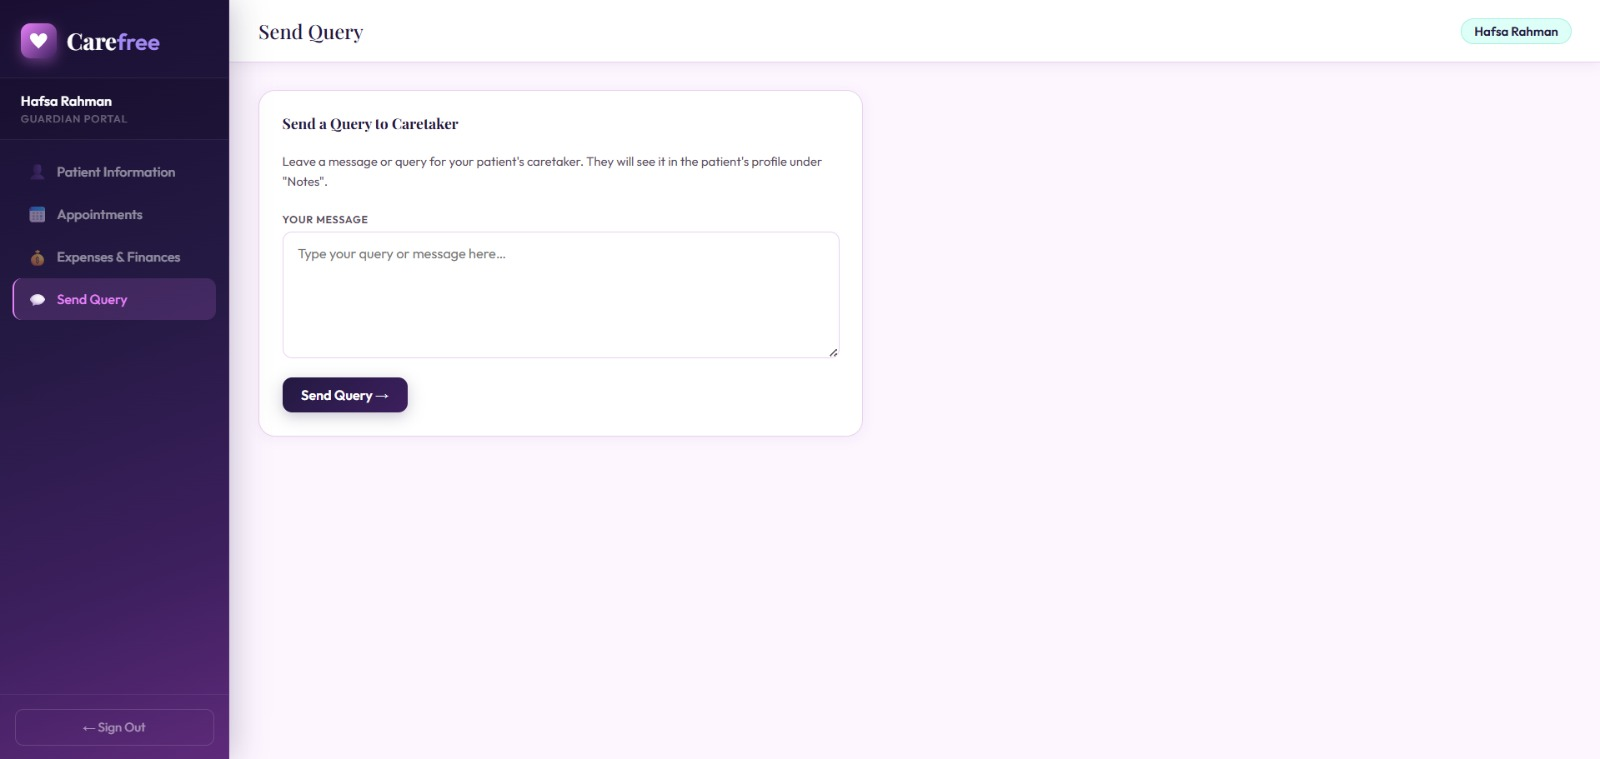
\includegraphics[width=0.85\textwidth]{external_schema/guardian_send_query.jpeg}
    \caption{Query Manager}
\end{figure}

\newpage

% ════════════════════════════════════════════════════════════════════════════
\section{Task 5 -- Code Quality Analysis (SonarQube Cloud)}
% ════════════════════════════════════════════════════════════════════════════

% Requires: static code analysis screenshots showing
% bugs, vulnerabilities, and code smells.

\begin{figure}[H]
    \centering
    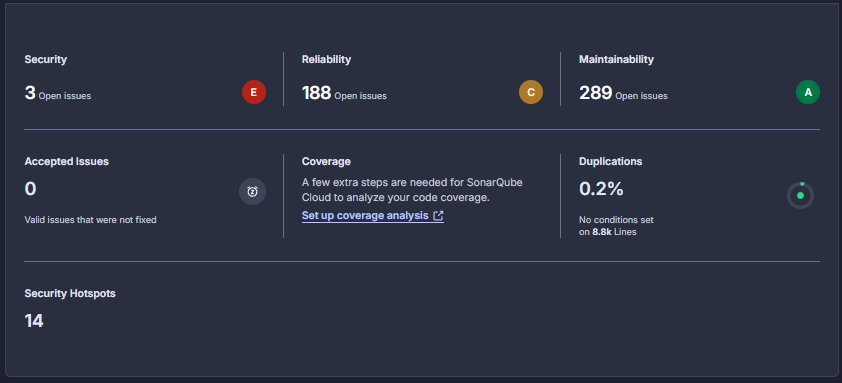
\includegraphics[width=\textwidth]{sonarqube/overview.png}
    \caption{SonarQube Cloud: Overview}
\end{figure}

\begin{figure}[H]
    \centering
    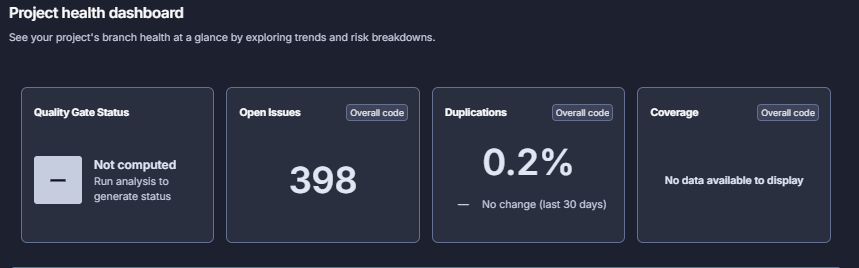
\includegraphics[width=\textwidth]{sonarqube/health_dashboard.png}
    \caption{SonarQube Cloud: Project Dashboard}
\end{figure}

\begin{figure}[H]
    \centering
    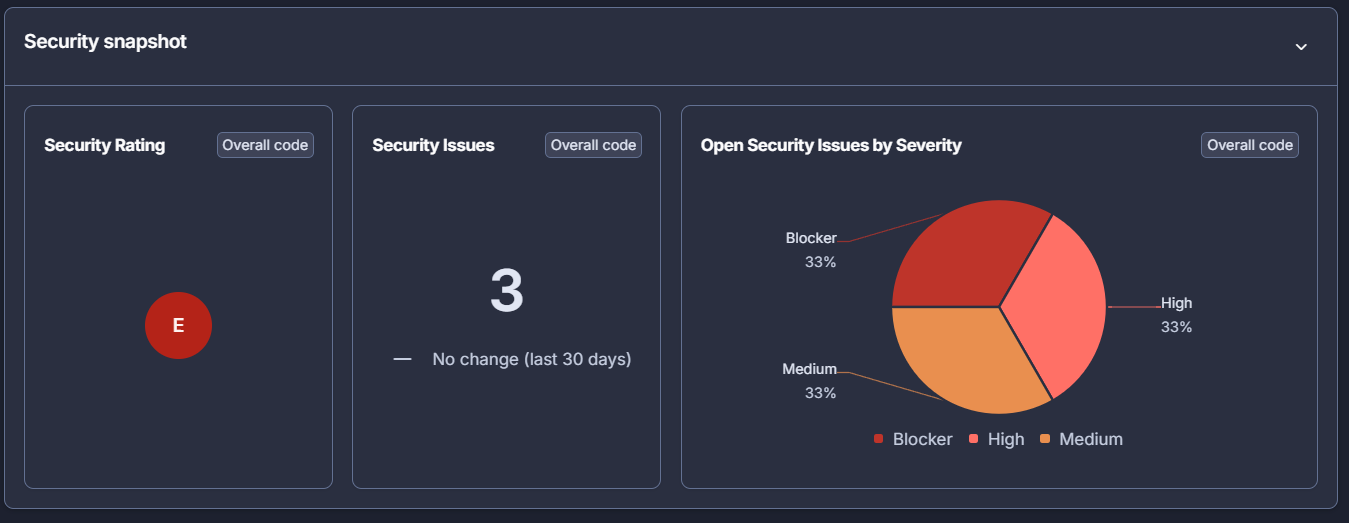
\includegraphics[width=\textwidth]{sonarqube/security_snapshot.png}
    \caption{SonarQube Cloud: Security Snapshot}
\end{figure}

\begin{figure}[H]
    \centering
    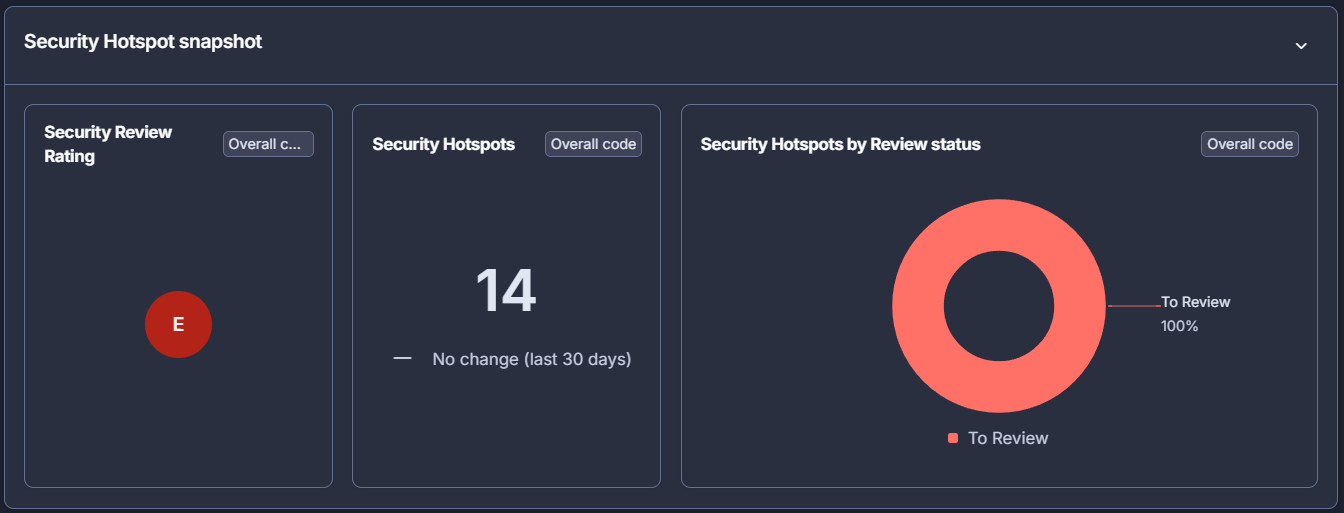
\includegraphics[width=\textwidth]{sonarqube/security_hotspot.png}
    \caption{SonarQube Cloud: Security Hotspot}
\end{figure}


\begin{figure}[H]
    \centering
    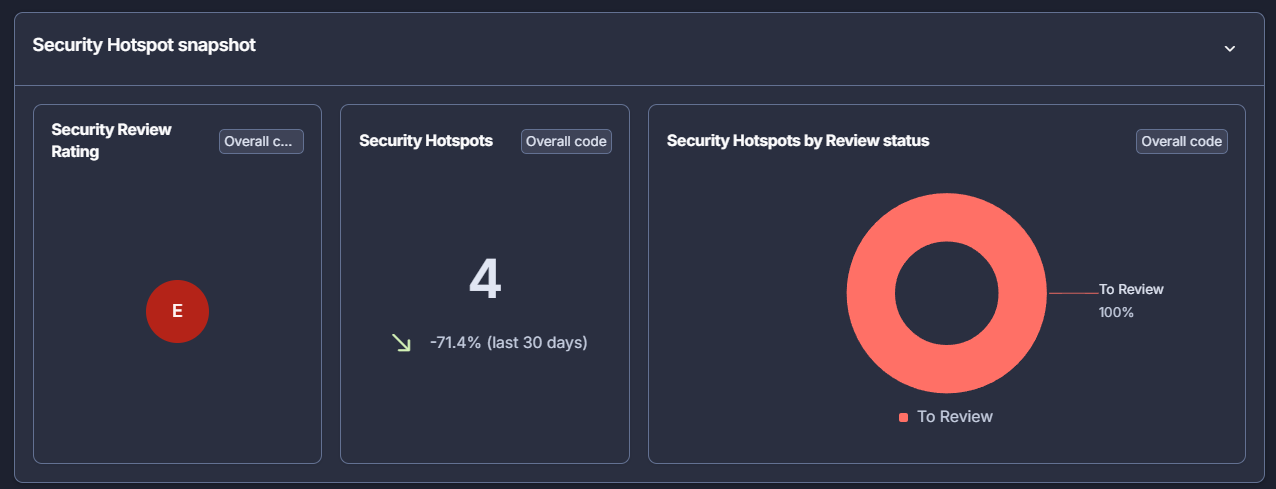
\includegraphics[width=\textwidth]{sonarqube/security_hotspot2.png}
    \caption{SonarQube Cloud: Security Hotspot after edition}
\end{figure}

\begin{figure}[H]
    \centering
    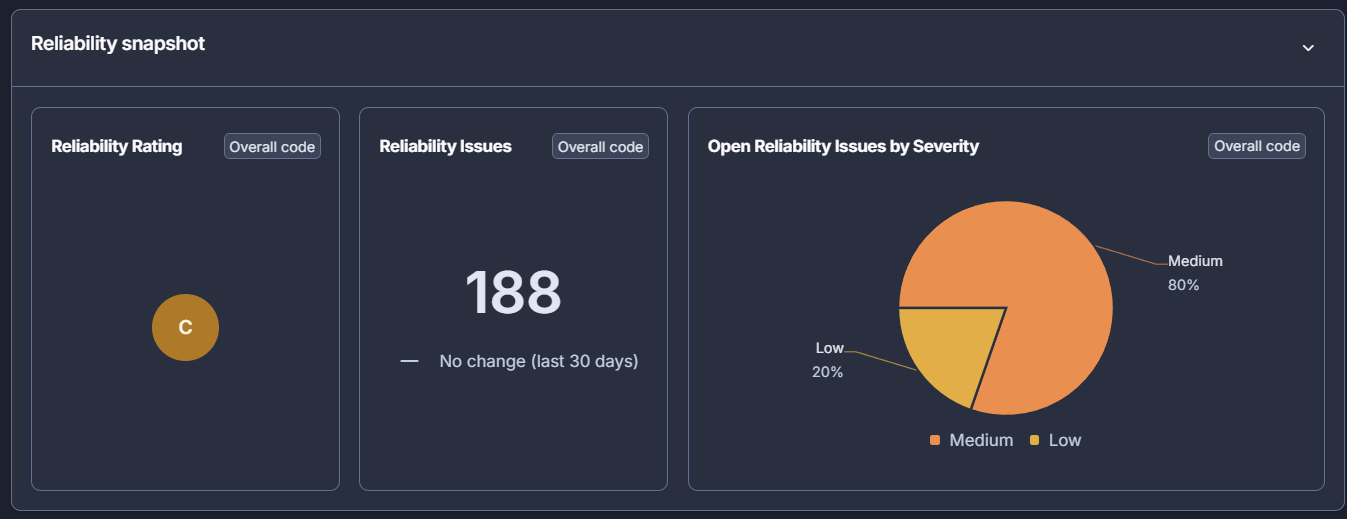
\includegraphics[width=\textwidth]{sonarqube/reliability.png}
    \caption{SonarQube Cloud: Reliability Overview}
\end{figure}

\begin{figure}[H]
    \centering
    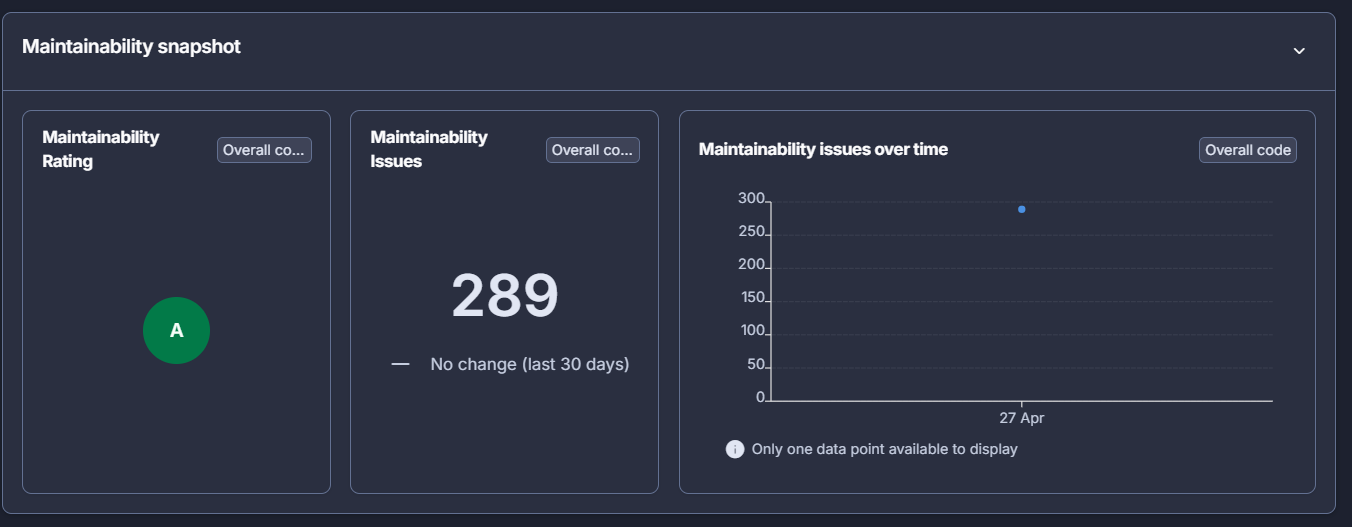
\includegraphics[width=\textwidth]{sonarqube/maintainability.png}
    \caption{SonarQube Cloud: Maintainability Overview}
\end{figure}
\begin{figure}[H]
    \centering
    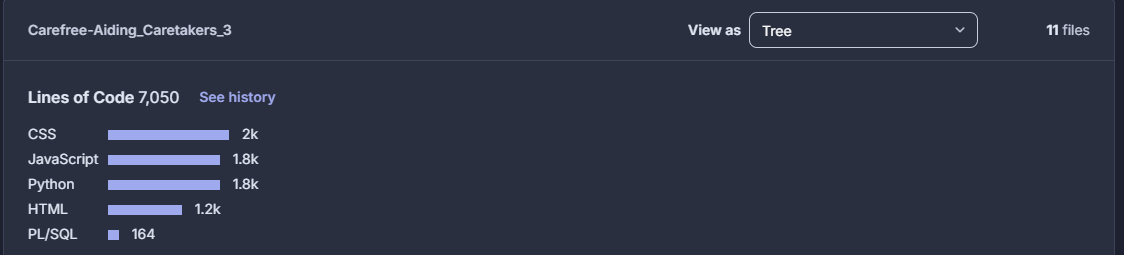
\includegraphics[width=\textwidth]{sonarqube/LOC.png}
    \caption{SonarQube Cloud: Lines of Code}
\end{figure}
\begin{figure}[H]
    \centering
    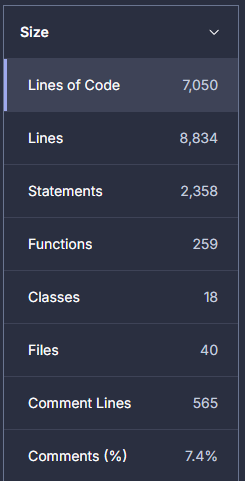
\includegraphics[width=0.25\textwidth]{sonarqube/LOC_distribution.png}
    \caption{SonarQube Cloud: LOC dostribution}
\end{figure}
\newpage

% ════════════════════════════════════════════════════════════════════════════
\section{Task 6 -- Manual Software Testing}
% ════════════════════════════════════════════════════════════════════════════

% Requires: test case description, test steps,
% expected result, and actual result.

\scriptsize
\setlength{\LTleft}{0pt}
\setlength{\LTright}{0pt}

\subsection{Unit Test Cases}
 
\begin{longtable}{|p{1cm}|p{2.5cm}|p{3.5cm}|p{3.5cm}|p{2cm}|p{1.2cm}|}
    \hline
    \textbf{TC ID} & \textbf{Description} & \textbf{Test Steps} & \textbf{Expected Result} & \textbf{Actual Result} & \textbf{Status} \\
    \hline
    \endfirsthead
    \hline
    \textbf{TC ID} & \textbf{Description} & \textbf{Test Steps} & \textbf{Expected Result} & \textbf{Actual Result} & \textbf{Status} \\
    \hline
    \endhead
 
    UT-01 & Login returns correct role for caretaker &
        1. Call \texttt{/api/login} with valid caretaker credentials.\newline
        2. Check response body. &
        Response contains \texttt{role='caretaker'}, \texttt{caretaker\_id}, and \texttt{name}. &
        Aligns with Expected & Pass \\
    \hline
 
    UT-02 & Login rejects wrong password &
        1. Call \texttt{/api/login} with valid username and incorrect password. &
        API returns 401 with `Invalid credentials' message. &
        Aligns with Expected & Pass \\
    \hline
 
    UT-03 & Login rejects unknown username &
        1. Call \texttt{/api/login} with a username not in the database. &
        API returns 401 with `Invalid credentials' message. &
        Aligns with Expected & Pass \\
    \hline
 
    UT-04 & Signup generates unique caretaker ID &
        1. Call \texttt{/api/caretaker} POST twice with different names. &
        Both succeed and return different CaretakerIDs. &
        Aligns with Expected & Pass \\
    \hline
 
    UT-05 & Signup rejects non-numeric contact &
        1. Call \texttt{/api/caretaker} POST with \texttt{contact='abc123'}. &
        API returns 400 with `Contact number must contain only digits'. &
        Aligns with Expected & Pass \\
    \hline
 
    UT-06 & Patient creation returns guardian password &
        1. Call \texttt{/api/patient} POST with all required fields including guardian details. &
        Response contains \texttt{patient\_id}, \texttt{guardian\_id}, and \texttt{guardian\_password}. &
        Aligns with Expected & Pass \\
    \hline
 
    UT-07 & Patient creation rejects guardian contact not 11 digits &
        1. Call \texttt{/api/patient} POST with \texttt{guardian\_contact='12345'}. &
        API returns 400 with validation error about contact length. &
        Aligns with Expected & Pass \\
    \hline
 
    UT-08 & Patient creation rejects negative age, weight, height &
        1. Call \texttt{/api/patient} POST with \texttt{age=-5}, \texttt{height=-170}, \texttt{weight=-50}. &
        API returns 400 with `Age/Height/Weight must be a positive integer'. &
        Aligns with Expected & Pass \\
    \hline
 
    UT-09 & Get patient returns all guardian fields via JOIN &
        1. Call \texttt{/api/patient/\{pid\}} for an existing patient. &
        Response includes \texttt{guardian\_name}, \texttt{guardian\_contact}, \texttt{relation}, \texttt{guardian\_comment}. &
        Aligns with Expected & Pass \\
    \hline
 
    UT-10 & Get patients returns only caretaker's own patients &
        1. Create two caretakers each with one patient.\newline
        2. Call \texttt{/api/patients/\{cid\}} for Caretaker A. &
        Only Caretaker A's patient is returned. &
        Aligns with Expected & Pass \\
    \hline
 
    UT-11 & Task creation returns valid task\_id &
        1. Call \texttt{/api/task} POST with all required fields and a future datetime. &
        Response contains \texttt{task\_id} as a positive integer. &
        Aligns with Expected & Pass \\
    \hline
 
    UT-12 & Task priority ordering is correct &
        1. Create High, Medium, and Low priority tasks for the same patient.\newline
        2. Call \texttt{/api/tasks/\{pid\}}. &
        Tasks returned: High first, Medium second, Low last. &
        Aligns with Expected & Pass \\
    \hline
 
    UT-13 & Task filter Today returns only today's tasks &
        1. Create tasks due today, tomorrow, and next week.\newline
        2. Call \texttt{/api/tasks/\{pid\}?filter=Today}. &
        Only the task due today is returned. &
        Aligns with Expected & Pass \\
    \hline
 
    UT-14 & Appointment creation rejects past datetime &
        1. Call \texttt{/api/appointment} POST with a past \texttt{datetime\_val}. &
        API returns 400 with `Appointments cannot be scheduled in the past'. &
        Aligns with Expected & Pass \\
    \hline
 
    UT-15 & Appointment creation inserts new doctor if absent &
        1. Call \texttt{/api/appointment} POST with a doctor name not in the Doctor table. &
        Appointment created and a new Doctor record inserted. &
        Aligns with Expected & Pass \\
    \hline
 
    UT-16 & Get appointments returns doctor name via JOIN &
        1. Create an appointment.\newline
        2. Call \texttt{/api/appointments/\{pid\}}. &
        Response includes \texttt{doctor\_name} and \texttt{specialization}. &
        Aligns with Expected & Pass \\
    \hline
 
    UT-17 & Expense creation updates patient charges &
        1. Note patient's Charges value.\newline
        2. Call \texttt{/api/expense} POST with \texttt{amount=500}. &
        Patient's Charges field increases by 500. &
        Aligns with Expected & Pass \\
    \hline
 
    UT-18 & Expense deletion updates patient charges &
        1. Create an expense of amount 300.\newline
        2. Delete via \texttt{/api/expense/\{eid\}} DELETE. &
        Patient's Charges field decreases by 300. &
        Aligns with Expected & Pass \\
    \hline
 
    UT-19 & Get expenses returns correct calculated\_balance &
        1. Set patient balance to 1000.\newline
        2. Add expenses totalling 600.\newline
        3. Call \texttt{/api/expenses/\{pid\}}. &
        Response contains \texttt{calculated\_balance=400}. &
        Aligns with Expected & Pass \\
    \hline
 
    UT-20 & Vitals creation inserts into all three sub-tables &
        1. Call \texttt{/api/vitals} POST with all vital fields filled. &
        VitalsID returned; CardiacVitals, RespiratoryVitals, and OtherVitals all have a matching row. &
        Aligns with Expected & Pass \\
    \hline
 
    UT-21 & Vitals creation skips sub-table if fields are null &
        1. Call \texttt{/api/vitals} POST with only \texttt{pulse\_rate} filled. &
        Only CardiacVitals row created; other sub-tables have no orphan rows. &
        Aligns with Expected & Pass \\
    \hline
 
    UT-22 & Vitals deletion cascades to all sub-tables &
        1. Create a full vitals entry.\newline
        2. Call \texttt{/api/vitals/\{vid\}} DELETE. &
        Vitals row and all corresponding sub-table rows are deleted. &
        Aligns with Expected & Pass \\
    \hline
 
    UT-23 & Get symptoms returns predefined and custom separately &
        1. Add one predefined and one custom symptom for the same patient.\newline
        2. Call \texttt{/api/symptoms/\{pid\}}. &
        Response has separate \texttt{predefined} and \texttt{custom} arrays each with one entry. &
        Aligns with Expected & Pass \\
    \hline
 
    UT-24 & Predefined symptom rejected if not in master list &
        1. Call \texttt{/api/symptom/predefined} POST with a non-existent \texttt{symptom\_id}. &
        API returns 404 with `Symptom not found in master list'. &
        Aligns with Expected & Pass \\
    \hline
 
    UT-25 & Notification dismiss marks Is\_Sent=1 &
        1. Create a notification.\newline
        2. Call dismiss endpoint.\newline
        3. Call \texttt{/api/notifications/\{cid\}} GET. &
        Dismissed notification no longer appears in the GET response. &
        Aligns with Expected & Pass \\
    \hline
 
    UT-26 & Vitals chart updates when vitals are logged &
        1. Go to Vitals panel.\newline
        2. Select a patient and log vitals. &
        Chart updates to reflect the newly logged vitals. &
        Aligns with Expected & Pass \\
    \hline
 
    UT-27 & Symptoms donut chart updates when new symptom is added &
        1. Go to Symptoms panel.\newline
        2. Select a patient and log a symptom. &
        Chart updates to reflect the new symptom entry. &
        Aligns with Expected & Pass \\
    \hline
 
    UT-28 & Cost predictor chart updates when predictor is used &
        1. Go to Cost Predictor panel.\newline
        2. Select a patient and predict cost. &
        Chart updates to reflect the new prediction. &
        Aligns with Expected & Pass \\
    \hline
 
    UT-29 & Stress predictor chart updates on use &
        1. Go to Stress Predictor panel.\newline
        2. Select a patient and predict result. &
        Chart updates to reflect the new prediction. &
        Aligns with Expected & Pass \\
    \hline
 
    UT-30 & Dashboard charts update when patient is selected &
        1. Go to Dashboard.\newline
        2. Select a patient and refresh. &
        All charts update to reflect the selected patient's data. &
        Aligns with Expected & Pass \\
    \hline
 
\end{longtable}
 
 
\subsection{System Test Cases}
 
\begin{longtable}{|p{1cm}|p{2.5cm}|p{3.5cm}|p{3.5cm}|p{2cm}|p{1.2cm}|}
    \hline
    \textbf{TC ID} & \textbf{Description} & \textbf{Test Steps} & \textbf{Expected Result} & \textbf{Actual Result} & \textbf{Status} \\
    \hline
    \endfirsthead
    \hline
    \textbf{TC ID} & \textbf{Description} & \textbf{Test Steps} & \textbf{Expected Result} & \textbf{Actual Result} & \textbf{Status} \\
    \hline
    \endhead
 
    ST-01 & Creating a new caretaker account &
        1. Enter the required details to register.\newline
        2. Press the sign up button. &
        Caretaker directed to the dashboard. &
        Aligns with Expected & Pass \\
    \hline
 
    ST-02 & Caretaker adds a new patient &
        1. Enter the required patient details.\newline
        2. Click Add Patient. &
        Patient added to list; caretaker receives guardian credentials. &
        Aligns with Expected & Pass \\
    \hline
 
    ST-03 & Caretaker signs in with correct credentials &
        1. Enter the correct details.\newline
        2. Press Log In. &
        Caretaker directed to the dashboard. &
        Aligns with Expected & Pass \\
    \hline
 
    ST-04 & User signs in with incorrect credentials &
        1. Enter the wrong password.\newline
        2. Press Sign In. &
        Error message shown to user. &
        Aligns with Expected & Pass \\
    \hline
 
    ST-05 & Adding a patient with incomplete information &
        1. Leave out required fields.\newline
        2. Click Add Patient. &
        Error message urging the user to complete all fields. &
        Aligns with Expected & Pass \\
    \hline
 
    ST-06 & Caretaker edits an existing patient's profile &
        1. Choose the patient's profile.\newline
        2. Edit required information.\newline
        3. Save changes. &
        Patient information updated and shown immediately. &
        Aligns with Expected & Pass \\
    \hline
 
    ST-07 & Caretaker deletes a patient &
        1. Choose the patient's profile.\newline
        2. Press Delete.\newline
        3. Confirm the action. &
        Patient removed from list; tasks, appointments, and expenses deleted via cascade. &
        Aligns with Expected & Pass \\
    \hline
 
    ST-08 & Users view patient details &
        1. Choose a patient ID and view their details. &
        Redirected to patient information with options to insert, update, etc. &
        Aligns with Expected & Pass \\
    \hline
 
    ST-09 & Caretaker creates a task with a past date &
        1. Enter required details with a past date.\newline
        2. Press Create Task. &
        Task created; table displays the next upcoming occurrence date. &
        Aligns with Expected & Pass \\
    \hline
 
    ST-10 & Caretaker views all tasks &
        1. Navigate to the Task section via the dashboard. &
        All tasks displayed with their details. &
        Aligns with Expected & Pass \\
    \hline
 
    ST-11 & Caretaker creates a task &
        1. Enter required details.\newline
        2. Press Create Task. &
        Task added and appears in the list. &
        Aligns with Expected & Pass \\
    \hline
 
    ST-12 & Caretaker creates an appointment &
        1. Enter required details.\newline
        2. Press Create Appointment. &
        Appointment added and appears in the list. &
        Aligns with Expected & Pass \\
    \hline
 
    ST-13 & Caretaker creates an appointment with a past date &
        1. Enter required details with a past date.\newline
        2. Press Create Appointment. &
        Error message urging the user to correct the date. &
        Aligns with Expected & Pass \\
    \hline
 
    ST-14 & Caretaker creates appointment without a doctor &
        1. Enter required details without selecting a doctor.\newline
        2. Press Create Appointment. &
        Application does not allow creation until a doctor is added or chosen. &
        Aligns with Expected & Pass \\
    \hline
 
    ST-15 & Caretaker changes existing doctor's specialization &
        1. Select an existing doctor and modify their specialization.\newline
        2. Press Create Appointment. &
        Appointment saved with the doctor's existing specialization in the system. &
        Aligns with Expected & Pass \\
    \hline
 
    ST-16 & Guardian views existing appointments &
        1. Navigate to Appointments after signing in. &
        Full list of appointments is displayed. &
        Aligns with Expected & Pass \\
    \hline
 
    ST-17 & Caretaker creates an expense &
        1. Enter required expense details.\newline
        2. Press Create Expense. &
        New expense added to the list. &
        Aligns with Expected & Pass \\
    \hline
 
    ST-18 & Caretaker deletes an expense &
        1. Select an expense.\newline
        2. Press Delete. &
        Confirmation prompt appears; confirming deletes the selected expense. &
        Aligns with Expected & Pass \\
    \hline
 
    ST-19 & Caretaker creates expense with negative amount &
        1. Enter a negative value for amount.\newline
        2. Press Create Expense. &
        Error message informing the user the amount cannot be negative. &
        Aligns with Expected & Pass \\
    \hline
 
    ST-20 & Caretaker creates expense with missing name or amount &
        1. Leave name or amount blank.\newline
        2. Press Create Expense. &
        Error message urging the user to complete the required information. &
        Aligns with Expected & Pass \\
    \hline
 
    ST-21 & Caretaker receives a task notification &
        1. Set a task 5 minutes from now with a frequency.\newline
        2. Wait. &
        Notification appears 5 minutes after the task was set. &
        Aligns with Expected & Pass \\
    \hline
 
    ST-22 & Caretaker receives an appointment notification &
        1. Create an appointment for the next day.\newline
        2. Check notification bell. &
        Notification appears immediately since appointment is within 24 hours. &
        Aligns with Expected & Pass \\
    \hline
 
    ST-23 & Caretaker creates a vital entry &
        1. Enter required vital details.\newline
        2. Press Add Vital. &
        Vital added to list and reflected in dashboard overview. &
        Aligns with Expected & Pass \\
    \hline
 
    ST-24 & Caretaker creates vital entry with missing fields &
        1. Leave some fields blank.\newline
        2. Press Add Vital. &
        Error message urging the user to complete the information. &
        Aligns with Expected & Pass \\
    \hline
 
    ST-25 & User views vitals overview for a patient &
        1. Navigate to dashboard.\newline
        2. Click on a patient row. &
        Vitals overview chart appears for the chosen patient. &
        Aligns with Expected & Pass \\
    \hline
 
    ST-26 & Caretaker logs a new custom symptom &
        1. Enter required details for a custom symptom.\newline
        2. Click Add Symptom. &
        New custom symptom logged in the patient's symptom list. &
        Aligns with Expected & Pass \\
    \hline
 
    ST-27 & User tries to add more than one vital per day &
        1. Select a patient.\newline
        2. Click Add Vital after already logging today. &
        Button disabled and displays ``Vitals for today is Logged''. &
        Aligns with Expected & Pass \\
    \hline
 
    ST-28 & Task shows next occurrence after time has passed &
        1. Add a task 2 minutes from now with Alternate frequency.\newline
        2. Wait, then reload. &
        Table shows the same time but date updated to the next alternate day. &
        Aligns with Expected & Pass \\
    \hline
 
    ST-29 & Search filter by patient name &
        1. Type the first letter of the patient's name in the search box. &
        Only patients matching the prefix are displayed. &
        Aligns with Expected & Pass \\
    \hline
 
    ST-30 & Add a predefined symptom from master list &
        1. Navigate to Symptoms panel.\newline
        2. Select a patient and click + Add Symptom.\newline
        3. Choose From Master List, select a symptom, and click Add Symptom. &
        Symptom appears tagged as predefined; severity chart updates. &
        Aligns with Expected & Pass \\
    \hline
 
    ST-31 & Adding vitals after deleting today's entry &
        1. Select a patient and delete existing vitals.\newline
        2. Click Add Vital. &
        New vitals log is allowed. &
        Aligns with Expected & Pass \\
    \hline
 
    ST-32 & Chart data pulls correctly across all panels &
        1. Select a patient and record full data in all chart panels.\newline
        2. Refresh to observe updates. &
        All charts update correctly pulling data across panels. &
        Aligns with Expected & Pass \\
    \hline
 
    ST-33 & Chart updation occurs across all panels &
        1. Select a patient.\newline
        2. Refresh. &
        All panels holding charts reflect updated data. &
        Aligns with Expected & Pass \\
    \hline
 
\end{longtable}
 
 
\subsection{Integration Test Cases}
 
\begin{longtable}{|p{1cm}|p{2.5cm}|p{3.5cm}|p{3.5cm}|p{2cm}|p{1.2cm}|}
    \hline
    \textbf{TC ID} & \textbf{Description} & \textbf{Test Steps} & \textbf{Expected Result} & \textbf{Actual Result} & \textbf{Status} \\
    \hline
    \endfirsthead
    \hline
    \textbf{TC ID} & \textbf{Description} & \textbf{Test Steps} & \textbf{Expected Result} & \textbf{Actual Result} & \textbf{Status} \\
    \hline
    \endhead
 
    IT-01 & Patient creation triggers guardian account &
        1. Create a patient with full guardian details.\newline
        2. Log out.\newline
        3. Log in as guardian using toast credentials. &
        Guardian can log in and sees correct patient info, appointments, and expenses. &
        Aligns with Expected & Pass \\
    \hline
 
    IT-02 & Patient deletion cascades across all modules &
        1. Create a patient with a task, appointment, expense, and vital.\newline
        2. Delete the patient. &
        Patient removed from dashboard; all linked records deleted; stats update. &
        Aligns with Expected & Pass \\
    \hline
 
    IT-03 & Task creation generates notification &
        1. Create a task 2 minutes in the future with Daily frequency.\newline
        2. Wait 2 minutes.\newline
        3. Open notification bell. &
        Notification appears with correct task name and patient reference. &
        Aligns with Expected & Pass \\
    \hline
 
    IT-04 & Appointment creation generates notification &
        1. Create an appointment for tomorrow.\newline
        2. Immediately check notification bell. &
        Notification appears immediately referencing doctor name and appointment time. &
        Aligns with Expected & Pass \\
    \hline
 
    IT-05 & Dashboard stats reflect real-time data &
        1. Note current counts for Tasks, Appointments, and Expenses.\newline
        2. Add one of each.\newline
        3. Return to dashboard. &
        All three stat cards show correctly incremented counts. &
        Aligns with Expected & Pass \\
    \hline
 
    IT-06 & Vitals entry appears in dashboard overview &
        1. Select a patient on dashboard.\newline
        2. Record a new vital entry.\newline
        3. Return to dashboard and click same patient row. &
        Vitals Overview chart updates to include new entry's data points. &
        Aligns with Expected & Pass \\
    \hline
 
    IT-07 & Cost predictor auto-fills from patient data &
        1. Add a patient with height, weight, smoker status, and region.\newline
        2. Navigate to Cost Predictor.\newline
        3. Select that patient from dropdown. &
        Age, BMI, smoker, and region fields correctly populated from stored data. &
        Aligns with Expected & Pass \\
    \hline
 
    IT-08 & Guardian views caretaker-added expenses &
        1. As caretaker, add two expenses for a patient.\newline
        2. Log out.\newline
        3. Log in as guardian for that patient. &
        Both expenses appear with correct names, categories, and amounts; balance reflects deductions. &
        Aligns with Expected & Pass \\
    \hline
 
    IT-09 & Guardian balance transfer reflects on caretaker side &
        1. As guardian, send a balance amount.\newline
        2. Log out.\newline
        3. Log in as caretaker and open expense panel. &
        Remaining balance reflects guardian's transfer. &
        Aligns with Expected & Pass \\
    \hline
 
    IT-10 & Task filter pill correctly scopes results &
        1. Create tasks due today, next week, and next month.\newline
        2. Click each filter pill (Today, This Week, This Month, All). &
        Each filter shows only tasks within that window; All shows all three. &
        Aligns with Expected & Pass \\
    \hline
 
    IT-11 & Appointment chart updates after new appointment &
        1. Note appointments chart for a patient.\newline
        2. Add a Consultation appointment.\newline
        3. Return to dashboard and click same patient row. &
        Consultation bar increments by 1; hover shows new appointment date. &
        Aligns with Expected & Pass \\
    \hline
 
    IT-12 & Symptom from master list appears in severity chart &
        1. Select a patient in Symptoms panel.\newline
        2. Add Chest Pain (High severity) from master list. &
        High severity bar increments in chart; symptom card appears in list. &
        Aligns with Expected & Pass \\
    \hline
 
    IT-13 & Switching patients updates all insight charts &
        1. Click Patient A row and note chart values.\newline
        2. Click Patient B row. &
        All charts re-render with Patient B's data; label updates accordingly. &
        Aligns with Expected & Pass \\
    \hline
 
    IT-14 & Recurring task notification reschedules after dismissal &
        1. Create a Daily task 1 minute from now.\newline
        2. Wait for and dismiss the notification.\newline
        3. Wait for next day's occurrence. &
        New notification for the same task appears for the next day. &
        Aligns with Expected & Pass \\
    \hline
 
    IT-15 & Caretaker cannot access another caretaker's patients &
        1. Sign up as two caretakers.\newline
        2. Add a patient under Caretaker A.\newline
        3. Log in as Caretaker B. &
        Caretaker B sees no patients, tasks, appointments, or expenses from Caretaker A. &
        Aligns with Expected & Pass \\
    \hline
 
    IT-16 & Vitals one-per-day restriction enforced &
        1. Record vitals for a patient.\newline
        2. Without changing date, click New Vital again. &
        Button disabled showing `Logged Today'; form submission also returns error. &
        Aligns with Expected & Pass \\
    \hline
 
    IT-17 & Deleting task or appointment removes its notification &
        1. Create a task with a scheduled notification.\newline
        2. Confirm notification appears.\newline
        3. Delete the task. &
        Linked notification disappears; bell count decrements. &
        Aligns with Expected & Pass \\
    \hline
 
\end{longtable}

\newpage

% ════════════════════════════════════════════════════════════════════════════
\section{Task 7 -- Version Control and Deployment}
% ════════════════════════════════════════════════════════════════════════════

% Requires: GitHub repository link and GitHub Pages deployment link.

\begin{itemize}
    \item \textbf{GitHub Repository:}
    \href{https://github.com/aizasamad164/Carefree-Aiding_Caretakers_3.git}{https://github.com/aizasamad164/Carefree-Aiding\_Caretakers\_3.git}
    \item \textbf{GitHub Pages:}
    \href{https://aizasamad164.github.io/Carefree-Aiding_Caretakers_3/}{https://aizasamad164.github.io/Carefree-Aiding\_Caretakers\_3/}
\end{itemize}

\begin{figure}[H]
    \centering
    \includegraphics[width=0.85\textwidth]{pages_1.jpeg}
    \caption{GitHub Pages -- Deployed Site}
\end{figure}

\begin{figure}[H]
    \centering
    \includegraphics[width=0.85\textwidth]{pages_2.jpeg}
    \caption{GitHub Pages -- Deployed Site}
\end{figure}

\begin{figure}[H]
    \centering
    \includegraphics[width=0.85\textwidth]{pages_3.jpeg}
    \caption{GitHub Pages -- Deployed Site}
\end{figure}

\end{document}